%
% Chapter 3
%
% Response eQTL-style HIRD paper

\chapter{Genetic architecture of transciptomic response to Pandemrix vaccine}
\label{ch:hird_reQTL}

% TODO check upreg and increased expression are consistent

% TODO: collab note 
% previous collab note applied since this is same dataset

\section{Introduction}

\subsection{Host genetic factors affecting influenza vaccine response}
\label{subsec:hird_reQTL_intro_geneticFactorsFluVaccine}

Many human traits are heritable and complex---response to vaccination is no exception.
Twin studies have demonstrated approximately \SIrange{30}{90}{\percent} heritability of antibody responses to many vaccines, including smallpox, hepatitis A and B, anthrax, pneumococcal, \textit{Haemophilus influenzae} type b (Hib), diphtheria-tetanus-pertussis (DTP), Bacillus Calmette--Guérin (BCG) \autocite{mooney2013SystemsImmunogeneticsVaccines,oconnor2013CharacterizingVaccineResponses,newport2015GeneticRegulationInfant,brodin2015VariationHumanImmune}.
Candidate gene studies and \glspl{GWAS} have identified multiple genetic associations with antibody response \autocite{mooney2013SystemsImmunogeneticsVaccines,oconnor2013CharacterizingVaccineResponses,mentzer2015SearchingHumanGenetic,linnik2016ImpactHostGenetic}, 
including replicated associations 
for hepatitis B vaccine in a haplotype block in the \gls{HLA} region encompassing \gene{HLA-DR} and \gene{BTNL2},
and for measles vaccine in an intron of a receptor known to interact with measles virus, \gene{CD46}.

In contrast, \textcite{brodin2015VariationHumanImmune} found anti-\gls{HA} antibody responses to seasonal influenza vaccine in 105 adult twin pairs (median age, \SI{44}{\year}) had no detectable heritabilty,
alongside a general decrease in heritability of most immune parameters with age.
They posited 
that the genetic contribution to response was overshadowed by environmental factors such as previous influenza vaccination or infection in adults, 
whereas the estimated heritability of the aforementioned vaccines was substantial
because they are vaccines against non-circulating pathogens, 
or are childhood vaccines for which heritability was assessed in young children with shorter immune history.

Nevertheless, a small number of candidate gene studies have identified genetic variants associated with antibody response to influenza vaccines \autocite{linnik2016ImpactHostGenetic}.
\textcite{gelder2002AssociationsHumanLeukocyte} ($n=73$) identified associations between \gls{HLA} alleles in \gene{HLA-DRB1} and \gene{HLA-DQB1} with \gls{HAI} seroconversion after \gls{TIV};
\textcite{moss2013CorrelationHumanLeukocyte} ($n=185$) also found associations between \gls{HLA} class II alleles (HLA-DRB1*04:01 and HLA-DPB1*04:01) and \gls{HAI} seroconversion after seasonal influenza vaccination.
\textcite{poland2008ImmunogeneticsSeasonalInfluenza} ($n=184$) tested HLA alleles, and \glspl{SNP} in coding and regulatory regions of cytokine or cytokine receptor genes, for association with post-\gls{TIV} \gls{HAI} titres specific to H1 and H3 subtypes (two of the components in the trivalent vaccine).
They reported nominally significant associations for two \gene{HLA-A} alleles with H1-specific titres,
six \glspl{SNP} associations with H1-specific titres
and ten \glspl{SNP} associations with H3-specific titres.
\textcite{egli2014IL28BKeyRegulator} ($n=196$) identified a \gls{SNP} upstream of \gene{IFNL3} (rs8099917) to be associated with seroconversion post-\gls{TIV},
and also found the \gls{SNP} to be an \gls{eQTL} for \gene{IFNL3} expression in H1N1-stimulated \glspl{PBMC} in a second cohort ($n=49$).
Lastly, \textcite{avnir2016IGHV169PolymorphismModulates} focused on a coding variant (rs55891010) in the part of \gene{IGHV1-69} that encodes the \gls{CDR} of broadly neutralising antibodies that bind influenza \gls{HA}.
One month after H5N1 avian influenza vaccination ($n=85$), associations were detected with usage of \gene{IGHV1-69} in the antibody repertoire,
and serum antibody binding efficiency to H5N1 \gls{HA}.
The associations listed above have all been found in small cohorts and have not been validated by subsequent studies,
so it remains unknown whether robust genetic associations with antibody response to influenza vaccines exist.

% NOTE: never mind the cellular response
%
% Genetics affects cellular response to other vaccines.
% DOI: 10.1128/CMR.00084-18
% Different ethnic groups living in the same location have varied responses to vaccination (64, 89, 161–166) and decline of antibodies (89), indicating a genetic influence on vaccine responses. Studies of twins estimate the degree of heritability to be 36 to 90% for humoral responses (167–173) and 39 to 90% for cellular responses, depending on the specific vaccine (167, 169) (Table 3).

% Adverse events genetics
% Also, genetics of phenotypes such as adverse events have been studied e.g. \url{https://pubmed.ncbi.nlm.nih.gov/25344690/}, ollila2017GeneticsVaccinationrelatedNarcolepsy

\subsection{\Glsfmtfullpl{reQTL} following influenza vaccination}

Host genetic variation could play a causal role in influenza vaccine response by altering the expression of genes as \glspl{eQTL}.
As mentioned in \cref{subsec:intro_contextDependenteQTL} and \cref{subsec:intro_reQTL}, the effect sizes of \glspl{eQTL} can be highly context-dependent,
and many \glspl{eQTL} in the immune system are \glspl{reQTL} only detectable after stimulation, not at baseline.
% \gls{eQTL} can have condition-specificity: an interaction between their effect on expression and different environmental contexts such as tissue or cell type\autocite{albert2015RoleRegulatoryVariation,vandiedonck2017GeneticAssociationMolecular}.
% The mechanisms by which \glspl{eQTL} interact with environment are of great interest;
% for example, cell type-specificity can inform us about how expression is regulated in a cell type-specific manner\autocite{kim-hellmuth2020CellTypeSpecific}.
% In a vaccination context, an important subset of context-dependent
% environment-interacting eQTLs are \glspl{reQTL}, defined as an eQTL whose effect interacts with external stimulation or perturbation.
% As the pre- and post-stimulation environments are separated in time, a possible mechanism that leads to the observation of reQTL is a genotype-dependent change in gene expression between timepoints,
% which may underlie genotype-dependent differences in antibody phenotypes.
\Glspl{reQTL} can be mapped considering a vaccination as an \textit{in vivo} immune stimulation.
This usually involves measuring the transcriptome of immune cells before and after vaccination in genotyped individuals,
then testing for genotype-dependent changes in expression.
As expression is a key molecular intermediate between genotype and phenotype,
a genotype-dependent change in expression after vaccination may be a mechanism mediating genotype-dependent vaccine antibody responses.

As reviewed in \cref{subsec:intro_reQTL},
few \textit{in vivo} \gls{reQTL} studies have been conducted,
and even fewer studies have been conducted where the \textit{in vivo} stimulation is vaccination,
despite the potential for learning about genetic regulation of vaccine-induced expression responses.
To my knowledge, there is only one such study: by \textcite{franco2013IntegrativeGenomicAnalysis} on response to seasonal inactivated \gls{TIV}.
\textcite{franco2013IntegrativeGenomicAnalysis} enrolled healthy Europeans adults into discovery ($n=119$ males) and validation ($n=128$ females) cohorts in two consecutive influenza seasons\footnote{Sex-dependence of effects was not addressed.}.
In each cohort, peripheral blood gene expression was measured by expression array on day 0 (baseline); and on days 1, 3, and 14 post-vaccination.
Serum \gls{HAI} and \gls{MN} titres were measured at days 0, 14, and 28 against each of the three vaccine components.
The \gls{TRI} \autocite{bucasas2011EarlyPatternsGene} was computed from these titres as a single measure of antibody response adjusted for baseline titres.
Genotyping was done by genotyping array.

\textit{Cis}-\gls{eQTL} were mapped using a linear mixed model jointly over all four days,
with day, genotype, day-genotype interaction, and a random intercept for individual as predictors; and gene expression the response variable.
This resulted in 467 \gls{eQTL} for 78 genes replicated in both cohorts,
with a significant day effect (indicating the gene was differentially expressed post-vaccination)
and a significant genotype effect (indicating the \gls{eQTL} effect).
To call \glspl{reQTL}, \glspl{eQTL} were also mapped separately for each day with a linear model including only genotype as a predictor,
from which the model $R^2$ was computed as a rough measure of the variance in expression explained by the \gls{eQTL} at each day.
\textcite{franco2013IntegrativeGenomicAnalysis} then computed delta-$R^2$: the maximum absolute deviation of the three post-vaccination $R^2$s from the day 0 $R^2$.
Out of the \glspl{eQTL} that replicated in both cohorts, 
146 \glspl{eQTL} for 34 genes ranked above the 99th percentile of the delta-$R^2$ distribution were defined as \glspl{reQTL}.
The union of the 78 and 34 genes from the above analyses (98 genes with \gls{DGE} and an \gls{eQTL}; or a \gls{reQTL}) was enriched for pathways and gene sets related to  
antigen processing and presentation, CD8\textsuperscript{+} T cell-mediated apoptosis, \gls{DC} maturation and function, and membrane trafficking.

Lastly, integrating antibody titre data,
they filtered down 20 gene with expression correlated to \gls{TRI} at any day, 
with an \gls{eQTL}, 
and with either post-vaccination differential expression \emph{or} a \gls{reQTL} effect.
% Their written conclusion was that: \enquote{these [20] loci have the strongest evidence of genetic variation influencing the immune response to the vaccine}, but due to the final \enquote{or} in their filtering criteria...
% TAP2, SNX29, FGD2, NAPSA, NAPSB, GM2A, C1orf85, JUP, FBLN5, CHST13, DIP2A, PAM, D4S234E, C3AR1, HERC2, LST1, LRRC37A4, OAS1, RPL14, and DYNLT1.
Seven genes out of these 20 were
antigen transport, processing, or presentation in \glspl{APC}:
\gene{NAPSA}, \gene{C1orf85}, \gene{GM2A}, \gene{SNX29}, \gene{FGD2}, \gene{TAP2}, and \gene{DYNLT1}.

Critically, \textcite{franco2013IntegrativeGenomicAnalysis} recognised that just assessing overlap of multiple filtering criteria does not allow them to infer the direction of causal relationships between genetic variation, expression and \gls{TRI}.
They attempted a model comparison with the CIT \autocite{millstein2009DisentanglingMolecularRelationships} to resolve the directionality of association between expression and \gls{TRI}, but unfortunately concluded there was only \textapprox{\SI{60}{\percent}} power at the total sample size of $n=247$.
Nevertheless, the study is proof of concept that integration of genotype, expression and antibody response data in an \textit{in vivo} \gls{reQTL} framework can be of suggestive genes under genetic regulation likely to be involved in vaccine response.

\subsection{Chapter summary}

The \gls{HIRD} cohort represents a unique opportunity for detecting genetic contributions to influenza vaccine response.
Similar to \textcite{franco2013IntegrativeGenomicAnalysis},
expression, antibody response, and genotypes are all available for the same individuals.
As Pandemrix is against a pandemic strain that had not been in seasonal circulation for decades at the time of cohort recruitment, 
responses will be less driven by individual immune history,
so power to detect genetic associations is expected to be greater.
% The cohort is too small for GWAS, so here expression.
% The only genetic factor measured was HLA haplotype, which did not associate with any other parameters measured.
In \cref{ch:hird_DGE}, I characterised differential gene expression induced by Pandemrix, as well as expression associations with antibody titres.
% For seasonal influenza vaccines, the contribution is small: antibody responses in adults are largely driven by non-genetic influences such as previous influenza vaccination or infection\autocite{brodin2015VariationHumanImmune}.
% As the Pandemrix vaccine is against a pandemic strain that was not in seasonal circulation at the time the \gls{HIRD} cohort was recruited (2010-11),
% with individuals mounting an expression response that was not recall-dominated \autocite{sobolev2016AdjuvantedInfluenzaH1N1Vaccination},
% the relative contribution of genetic factors to Pandemrix response may be greater.
In this chapter---given that \gls{HIRD} is too small for a direct \gls{GWAS} of antibody response---I focus on the genetic contribution to expression response.
I apply the \textit{in vivo} \gls{reQTL} framework, 
aiming to characterise the association of common genetic variants with expression across multiple timepoints,
and pinpoint genes important to Pandemrix response.
% I map cis-\gls{eQTL} within each timepoint, accounting for ancestry, cell type composition, and unmeasured covariates, then call shared and \gls{reQTL} effects across timepoints from a joint model.
% Many of the strongest reQTL effects involve opposite signed effects on expression for the same variant at different timepoints.
% I detect a strong day 1 specific reQTL effect at \gene{ADCY3}.
% Through modelling interaction of reQTL with cell type abundance estimates and statistical colocalisation with cell type-specific QTL datasets,
% the reQTL signal was determined to be a monocyte-specific effect likely driven by increase monocyte abundance at day 1.

\section{Methods}
\label{sec:hird_reQTL_methods}

\subsection{Overall strategy for \glsfmtshortpl{reQTL} mapping}
\label{subsec:hird_reQTL_overall_strategy}

A plethora of approaches to mapping \glspl{eQTL} with linear models exist; each with its own advantages, disadvantages, and assumptions.
When the task is also to define \gls{reQTL} between multiple conditions, the diversity of possible approaches multiplies further.
Here I will discuss aspects of the data and available methodologies that led to the final modelling strategy in this study.

\subsubsection{Adjusting for population structure using \glsfmtlongpl{LMM}}

Population structure occurs when the samples in a study are not independent, but structured due to genetic relatedness.
Genetic association studies assume that the individuals in a sample are unrelated (or at least sufficiently distantly related) \autocite{astle2009PopulationStructureCryptic,sillanpaa2011OverviewTechniquesAccount,sul2018PopulationStructureGenetic}.
Relatedness, and thus population structure, occurs at different scales.
Population stratification refers to systematic differences in allele frequencies and genetic background between human populations due to demographic history.
This represents large-scale structure where individuals are related due to shared ancestry \autocite{price2010NewApproachesPopulation,sillanpaa2011OverviewTechniquesAccount}.
At a smaller scale, sample individuals can be related due to being in the same family.
The presence of more relatedness in a sample than is assumed is the problem of cryptic relatedness \autocite{astle2009PopulationStructureCryptic,sillanpaa2011OverviewTechniquesAccount,sul2018PopulationStructureGenetic};
this can be at any scale, but more often the term refers to recent relatedness.
% NOTE: fine scale population structure
% If one assumes humans across the globe are a single randomly mating population, it would result in only a 5–15% average error when predicting the proportion of observed heterozygotes at a locus. This closeness to an idealized randomly mating population is one vestige of how little evolutionary time has passed since the common origin of all humans in Africa. The departure from random mating predictions due to population differentiation has a classic quantitative measure, called FST, which appropriately takes on values of 5–15% in global samples of human populations [1, 2, 3••]. If one zooms in within continental regions of the globe, FST tends to be even lower, regularly taking values below 1%, a threshold which we use here informally to define ‘fine-scale structure’.

In the context of \gls{eQTL} mapping (and genetic association studies in general), 
where the aim is to assess the effect of a single genetic variant on expression, 
there is potential for confounding.
The issue (also reviewed elsewhere \autocite{sul2018PopulationStructureGenetic,golan2018MixedModelsCaseControl}) is that we fit a marginal model to estimate the effect of a single variant $x_k$ on the phenotype $y$:
\begin{equation}
    y = \mu + \beta_k x_k + \epsilon
    \label{eq:hird_reQTL_gwas_model_marginal}
\end{equation}
where $\mu$ is the intercept,
and $\epsilon \sim N(0, \sigma_e^2 I)$ is the error term that represents environmental and stochastic sources of variation,
The variance-covariance matrix for error term is a scalar matrix, 
encoding the classic regression assumptions of homoscedasticity and uncorrelated errors.
A more appropriate data generating model is:
\begin{equation}
    y = \mu + \beta_k x_k + G + \epsilon
    \label{eq:hird_reQTL_gwas_model_full}
\end{equation}
where $G = \sum_{i \neq k}{\beta_i x_i}$ represents the effect of the genetic background at all other variants.
As many variants can be expected to affect a complex polygenic trait, $G$ has some causal effect on $y$.
Population structure means there can be a shared cause of $G$ and $x_k$ such as ancestry.
This opens a backdoor path $x_k \leftarrow \text{ancestry} \rightarrow G \rightarrow y$,
confounding the relationship between $x_k$ and $y$.
In \cref{eq:hird_reQTL_gwas_model_marginal},
% the error term will actually represent $G + \epsilon$.
% the error term and $x_k$ become correlated (endogeneity),
when one estimates the coefficients,
the effects of the omitted variable $G$ will be attributed to $x_k$,
resulting in spurious associations and genomic inflation of test statistics \autocite{price2010NewApproachesPopulation}.
Here, $G$ represents exactly the confounding due to genetic background,
but there are other possible confounders,
such as shared environmental factors that differ systematically between populations \autocite{vilhjalmsson2013NatureConfoundingGenomewide}.
A popular approach to avoid confounding is to include genotype \glspl{PC} (a proxy for ancestry) as fixed effects in the regression \autocite{price2006PrincipalComponentsAnalysis,eu-ahsunthornwattana2014ComparisonMethodsAccount},
thus blocking the backdoor path from $x_k$ to $y$.
The genotype \glspl{PC} themselves also act as proxies to adjust for environmental confounders.

Unfortunately, genotype \glspl{PC} alone cannot account for smaller-scale population structure \autocite{price2010NewApproachesPopulation}.
An approach that can explicitly model such population structure is the \gls{LMM} \autocite{price2010NewApproachesPopulation,eu-ahsunthornwattana2014ComparisonMethodsAccount,golan2018MixedModelsCaseControl},
which expresses the idea that more genetically correlated individuals are expected to be more phenotypically correlated \autocite{vilhjalmsson2013NatureConfoundingGenomewide}.
A typical model form is:
\begin{equation}
    y = \mu + \beta_k x_k + u + \epsilon
    \label{eq:hird_reQTL_gwas_model_lmm}
\end{equation}
where random effect $u \sim N(0, \sigma_g^2 K)$
has a variance-covariance matrix proportional to the genetic correlation between individuals, the kinship matrix $K$.
% Since the SNPs are correlated, due to the major genome-wide diffrences in allele frequencies between the populations, this results in a correlation between the tested SNP and the noise term.
This improves on \cref{eq:hird_reQTL_gwas_model_full} by recognising that the variants in $G$ are correlated.
$\sigma_g^2$ is often called the variance component; the larger it is, the more phenotypic variance is explained by genetic background \autocite{golan2018MixedModelsCaseControl}.
Although \glspl{LMM} were originally developed in the context of animal breeding, where $K$ is computed from a known pedigree,
it can also be estimated from genome-wide \gls{SNP} data \autocite{eu-ahsunthornwattana2014ComparisonMethodsAccount,sul2018PopulationStructureGenetic}.
\gls{SNP}-based relatedness values, unlike pedigree‐based kinships that range from 0 (unrelated) to 1 (self or identical twin), may be negative or greater than 1 \autocite{wang2014MarkerbasedEstimatesRelatedness}, but this does not affect their usage as part of the variance-covariance \glspl{LMM}.
%
% Also see: 
%
% 2018-11-26 notes in log
%
% https://twitter.com/A_A_Zaidi/status/1285578961356034049
% When structure has a recent origin, PCA or LMMs won't fully correct for stratification if the GRM is derived from common variants as they are older and not very informative about recent demographic history.
%
% We demonstrate that widely used approaches to adjust for population structure, including principal components analysis and mixed modelling with a random effect for a genetic relationship matrix, cannot fully account for the fine-scale geographical confounding in the UK Biobank.
% fine scale: https://academic.oup.com/hmg/article-abstract/doi/10.1093/hmg/ddaa157/5874041

In \gls{HIRD},
the genotype data were already filtered such that no pair of individuals are first-degree relatives or closer (\cref{subsec:hird_dge_genotype_preproc}),
but cryptic relatedness might remain.
The multi-ethnicity of the cohort means there is large-scale population structure from ancestry (\cref{fig:hird_genotype_pca_withHapmap}).
Genotype \glspl{PC} were computed to represent axes of variation due to ancestry.
These were included as covariates in \gls{DGE} analyses in \cref{ch:hird_DGE} to improve efficiency by explaining some variation in expression.
For \gls{eQTL} mapping in this chapter, I use both a random effect in an \gls{LMM} and \gls{PC} fixed effects to correct for population structure.
This may not be strictly necessary if the random effect can correct for large-scale structure, 
but does not seem to impact power or type I error rate \autocite{widmer2015FurtherImprovementsLinear},
and may have some benefits at \glspl{SNP} with very different allele distributions between populations (unusually differentiated) \autocite{price2010NewApproachesPopulation}.

% For list of various methods considered, also see 2018-03-05, 2018-07-25, 2018-07-27 etc. in log
The performance of various software implementations 
for kinship estimation from genome-wide \gls{SNP} data and \glspl{LMM} are highly comparable; 
the specific choice of implementation can usually be made on the basis of computational efficiency \autocite{eu-ahsunthornwattana2014ComparisonMethodsAccount}.
In this chapter, I use
\glspl{LMM} implemented in \software{LIMIX} \autocite{lippert2014LIMIXGeneticAnalysis}
with kinship matrices estimated by \software{LDAK} \autocite{speed2012ImprovedHeritabilityEstimation}.

\subsubsection{Multi-condition models}

Since the aim of this chapter is to identify genetic variation that affects expression response to vaccination, it may seem most direct to model the change in each individual's expression after vaccination as the response variable.
This approach has been applied for identification of condition-specific \gls{eQTL}, typically with the response taking units of log fold change between conditions (e.g. \autocite{maranville2011InteractionsGlucocorticoidTreatment,ackermann2013ImpactNaturalGenetic,shpak2014EQTLAnalysisHuman}).
Although potentially powerful if \gls{eQTL} effects are small and opposite between conditions\autocite{ackermann2013ImpactNaturalGenetic}, 
% TODO: although ackermann2013ImpactNaturalGenetic distinguishes dynamic, there is no structural diff between using the
% fold change vs interaction vs stratified, for example, suppose different individuals pre and post, it's really a matter of assumptions and efficiency.
it is analogous to the \enquote{change score} approach, which can suffer from regression to the mean (??), and increased uncertainty from the variance sum law if effects between conditions have positive covariance\autocite{allison1990ChangeScoresDependent,clifton2019CorrelationBaselineScore}.
% NOTE:
% https://journals.sagepub.com/doi/full/10.1177/1054773816666280
% Threats to Its Internal Validity and External Validity of One-Group Pretest–Posttest Design include regression to the mean.
%
% Step 1: why not intra-individual change score, why not ANCOVA, why strat and diff?
% half a century of debate
% https://digscholarship.unco.edu/cgi/viewcontent.cgi?article=1239&context=dissertations
% https://ruor.uottawa.ca/bitstream/10393/35843/3/Lemay_Julien_2017_Thesis.pdf

% TODO:
% in observational: https://www.tandfonline.com/doi/abs/10.1080/00273171.2013.831743?scroll=top&needAccess=true&journalCode=hmbr20
% in RCT: senn says equiv: https://www.google.com/url?sa=t&rct=j&q=&esrc=s&source=web&cd=&ved=2ahUKEwie_PK6vsvsAhXXRRUIHdUfD_wQFjAAegQIAxAC&url=http%3A%2F%2Fimaging.mrc-cbu.cam.ac.uk%2Fstatswiki%2FFAQ%2Frt1d%3Faction%3DAttachFile%26do%3Dget%26target%3Dsenn.ppt&usg=AOvVaw0Rp28syfyesdecEiQZw9x_
% pearl says: ?
% senn in observational: ?? https://onlinelibrary.wiley.com/doi/abs/10.1002/sim.2682
%
% \todo{upend change score bit, here expression is a y variable. compare all the options as glms etc.}
% TODO: Write both as special cases of glm, and highlight their different assumptions
% TODO: mention: in ch2, used residualised change score, here, different
% Our data structure is
% Over all approach is stratified
%
% 2 schools of thought. 50 years of debate
% Change score assigns special status, assumes a specific correlation
% ...
%
% Besides not even estimatejng the same effect
%
% Many other models reduce to change score
%
% Mixed is flexible, but overall aim aligns with change score
%
% Simplest application of developed eqtl methods

% joint method over interaction
%     large numbers of conditions, not practical to use interactions

% pros for split
%     limix not ok with repeated samples in kinship matrix
%     peer not directly applicable
    
% change score should ask average of individual diffs
% strat and interaction should ask diff in averages
% interaction is further borrowing info
%
% NOTE: see
% Senn: Statistical Issues in Drug Development
% 7.2.4 Is clinical relevance a relevant consideration when choosing whether to use change scores or raw outcomes as the efficacy measure?

% TODO:  
 % It is imperative to adjust for the baseline value anyway, using regression modeling (for reasons of bias reduction in observational studies and for maximizing power and precision in randomized trials).
 % Using each patient as her own control through calculation of a change score is worse than using no control if the baseline is noisy. If the correlation between baseline and follow-up measurement is less than 0.5, subtracting the baseline is worse than just analyzing the follow-up measurement.
 % http://biostat.mc.vanderbilt.edu/wiki/Main/MeasureChange

Instead, I map \glspl{eQTL} within each of three timepoint conditions (day 0 pre-vaccination, day 1, and day 7), and find \glspl{reQTL} by looking for \glspl{eQTL} that have different effects between conditions.
% TODO: would use ANCOVA here i.e. equiv to continuous covar in regression
% TODO it is not the case people act as their own controls, you can't observe the counterfactual outside of n of 1 trials
% more like soaking up some of the variation as within individual random effect, allowing more precise
% also see: https://blog.statsols.com/making-it-personal-n-of-1-trials-allowing-for-individuality-but-not-overdoing-it
% \todo{Can this really demonstrate genotype-dependent change in gene expression between timepoints? i.e. need understand how the change score/ANCOVA approaches differ from repeated measures ANOVA differ from the interaction/stratified approach I take?}
Unlike a test for difference implemented using a genotype-condition interaction term in a joint regression model, homoscedasticity of errors is not assumed for all conditions\autocite{clogg1995StatisticalMethodsComparing}
% See PMC4425538 : The method we have used did not account for heteroscedasticity while estimating the standard errors of the interaction term, which may lead to inflated statistics.
% TODO: equivalence is not straightforward, since of joint mashr downstream

% real killer is missing data for manova/ancova
% TODO: also MANOVA
% Instead of just accommodating unequal variances and covariance within a subject, the mixed models approach directly models the covariance structure of the multiple dependent variables.
% https://blogs.sas.com/content/sastraining/2011/02/02/the-punchline-manova-or-a-mixed-model/
% https://stats.stackexchange.com/questions/13197/differences-between-manova-and-repeated-measures-anova
% avoids sphericity http://www.discoveringstatistics.com/docs/sphericity.pdf
%
% But, we are interested in interaction, and this is not directly answered by manova (i.e. multivariate mode in limix)

% Independence: errors assoc with one observation are not correlated with erros of any other
% Homoscedasticity: Var y does not depend on x

% Step 2: why stratification/subgroup not interaction
% TODO interaction is more efficient under certain assumptions
%     https://stats.stackexchange.com/questions/332963/why-may-results-from-model-with-interaction-term-and-stratified-model-be-differe
% These models will consistently estimate the same thing only when the mean model is true.
% possible here since time is not treated as continuous
% https://stats.stackexchange.com/questions/93540/testing-equality-of-coefficients-from-two-different-regressions
    % I found the key difference is whether the assumption that the error variance is the same or not.
% https://stats.stackexchange.com/questions/55501/test-a-significant-difference-between-two-slope-values
    % The classic (and more statistically powerful) way of testing this is to combine both datasets into a single regression model and then include the area as an interaction term. See, for example, here:
    % http://www.theanalysisfactor.com/compare-regression-coefficients/
    % This is "more ... powerful" only if more restrictive assumptions apply. In particular, it assumes homoscedasticity of error variances. Often one would not want to assume that (without additional justification) and therefore would use something like the Welch or Satterthwaite t-test. – whuber♦ Mar 30 '16 at 21:46
%
% https://stats.stackexchange.com/questions/33692/joint-model-with-interaction-terms-vs-separate-regressions-for-a-group-comparis
%     The first model will fully interact gender with all other covariates in the model. Essentially, the effect of each covariate (b2, b3... bn). In the second model, the effect of gender is only interacted with your IV. So, assuming you have more covariates than just the IV and gender, this may drive somewhat different results.
% i.e. there are interactions between time and ALL VARIABLES
%
% whereas interaction model pools estimates (borrows info)
%
% cons:
% interaction gives direct p nominal value, we have to estimate
% but how to control for multiplicity?
%
% Statistical Approaches for Estimating Sex-Specific Effects in Endocrine Disruptors Research
% https://ehp.niehs.nih.gov/doi/10.1289/EHP334 < TODO
%
% also see homo: https://cris.maastrichtuniversity.nl/ws/files/11868404/799719.pdf
% TODO:
% really, pro is Simplicity
% Can do interactions
% Can do coloc
% Can use peer
% interaction with time fixed fx vs stratified
% \todo{interactions, apart from scalability genome wide, and additional complexity when also adding cell type and platform interactions, and assumption of homoscedascity between all groups}
% vs pooling power
%
% note intent to use joint modelling later, so as to not lose info and fall into jelly bean problem https://www.ahajournals.org/doi/10.1161/CIRCULATIONAHA.108.836601

% TODO: honestly given i used change score in ch2, the biggest motivator is probably practicality e.g. ability to use PEER

%
% DEPRECATED:
% How to meta-analyse? We are restricted to non-full Bayesian methods.
%
% See last paragraph of discussion in
% Kontopantelis, E., Springate, D. A., & Reeves, D. (2013). A Re-Analysis of the Cochrane Library Data: The Dangers of Unobserved Heterogeneity in Meta-Analyses. PLoS ONE, 8(7), e69930. https://doi.org/10.1371/journal.pone.0069930
% For small k, Sidik MVa or Ruhkin RBp recommended.
%
% metafor manual
% If, instead of the crude estimate, one wants to use a better apriori estimate, one can do so by passing this value via control=list(tau2.init=value)
% Sidik-Jonkman estimator, also called the ‘model error variance estimator’, is implemented in metafor (SJ method).
% Starts with an init estiamte of ri=sigma2i/tau2i i.e. ratio of study-specific and between-studies het variance, then updates.
% They recommend using Hedges [1], to init, but this is bad???
% We use mode of gamma as an apriori estimate of tau.
%
% 2.7.	Meta-analysis with metafor
% 2.7.1.	Per day, use rma(‘REML’) to fit random-effects model on association beta and beta_ste, per gene-SNP pair, using all timepoints from array/RNA-seq for that day
% 2.8.	eigenMT to get number of independent tests per gene
% 2.8.1.	split previously generated geneloc and snpsloc by chrom
% 2.8.2.	per chrom, run eigenMT on limix output (arbitrary day, since the set of snps cis to each gene does not vary by day)
% 2.9.	Compute hierarchical FDR
% 2.9.1.	Per day
% 2.9.1.1.	Use eigenMT estimates to apply local Bonferroni per gene
% 2.9.1.2.	Compute global BH FDR
Within each timepoint, recall the the \gls{HIRD} dataset includes expression measured by both array and \gls{RNAseq}.
As discussed in \cref{subsubsec:hird_dge_meta_methodChoice}, it is difficult to directly estimate the between-studies heterogeneity when the number of studies is small, 
and Bayesian meta-analysis was preferred for combining array and \gls{RNAseq} \gls{DGE} estimates.
% \todo{why I didn't just do a mega-analysis in chapter 2 then, given I haven't any evidence if it's better or worse than Bayesian meta-analysis in that context.}
That method does not scale to \gls{eQTL} analysis, where the number of tests is large, in the order of thousands of tests per gene, versus the handful \gls{DGE} contrasts per gene performed in \cref{ch:hird_DGE}.
Instead, I perform a mega-analysis within each timepoint, first merging array and \gls{RNAseq} expression estimates into a single matrix with ComBat \autocite{johnson2007AdjustingBatchEffects}.
TODO: related to previous paragraph
For comparison purposes, analyses were also run in the array and \gls{RNAseq} samples separately.
% \todo{add -7 note as with ch2}

Defining whether an \gls{eQTL} is shared between conditions can be a tricky business.
Naively, one can map \glspl{eQTL} separately in each condition, then assess the overlap of significant associations between conditions.
This underestimates sharing due to the difficulty of distinguishing true lack of sharing from missed discoveries,
as a consequence of incomplete power within each condition \autocite{flutre2013StatisticalFrameworkJoint,peters2016InsightGenotypePhenotypeAssociations}.
Condition-by-condition analysis also cannot borrow information across conditions for mapping shared associations\autocite{flutre2013StatisticalFrameworkJoint,urbut2018FlexibleStatisticalMethods,li2018HTeQTLIntegrativeExpression}.
Counterintuitively, a joint multivariate analysis may be more powerful even when associations are not shared across all conditions\autocite{stephens2013UnifiedFrameworkAssociation}.

% 2018-07-25 log: HIRD eQTL modelling possibilities
% General pattern of development:
% MANOVA < MetaTissue
% MetaTissue < JAGUAR < RECOV
% Metasoft < mashr
% eqtlbma < mashr
% MetaTissue < MT-eQTL < HT-eQTL
%
% Excellent history from the HT-eQTL paper https://bmcbioinformatics.biomedcentral.com/articles/10.1186/s12859-018-2088-3
% Recently, the NIH Common Fund’s Genotype-Tissue Expression (GTEx) project has undertaken a large-scale effort to collect and analyze eQTL data in multiple tissues on a growing set of human subjects, and there has been a concomitant development of methods for the analysis of such data.
% For example, Peterson et al. [3] and Bogomolov et al. [4] developed new error control procedures to control false discovery rates at different levels of resolution (e.g., at the SNP level or the gene level) for eQTL analysis.
% The methods have been used to identify genes whose expression is regulated by SNPs (eGenes), or SNPs that affect the expression levels of multiple genes (eSNPs).
% However, the methods only concern how to reduce the number of hypotheses in a hierarchical structure, but cannot effectively borrow strength across tissues to enhance eQTL discoveries.
% Lewin et al. [5], Sul et al. [6] and Han et al. [7] developed regression-based methods via Bayesian multivariate regression and random-effects models.
% The models accommodate data from multiple tissues simultaneously, and integrate information across tissues for eQTL detection.
% However, a potential drawback is that they only focus on one gene or gene-SNP pair at a time, and fail to leverage information across different gene-SNP pairs.
% Flutre et al. [8] and Li et al. [9] developed hierarchical Bayesian models to model summary statistics across multiple tissues.
% The models capture the marginal distribution of each gene-SNP pair with interpretable parameters, and explicitly characterize heterogenous eQTL configurations in multiple tissues.
% However, the model fitting is computationally expensive and cannot scale to a large number of tissues.
% Recently, Urbut et al. [10] proposed an ad hoc approach based on shrinkage to improve the scalability of the Bayesian models.
% However, the procedure is subject to overfitting and the model parameters are hard to interpret.
%
A variety of models have been employed for joint \gls{eQTL} mapping, including
the use of classical multivariate methods such as \gls{MANOVA} \autocite{kim2014CharacterizingGeneticBasis},
frequentist meta-analyses (e.g. Meta-Tissue \autocite{sul2013EffectivelyIdentifyingEQTLs}, METASOFT \autocite{han2011RandomEffectsModelAimed}), 
and Bayesian models (e.g. eQtlBma \autocite{flutre2013StatisticalFrameworkJoint}, MT-HESS \autocite{lewin2016MTHESSEfficientBayesian}, MT-eQTL \autocite{li2018EmpiricalBayesApproach}).
Joint mapping has been repeatedly demonstrated to be more powerful than condition-by-condition analysis,
and recent methods are now computationally efficient when scaling to large numbers of conditions and variants tested (e.g. RECOV \autocite{duong2017ApplyingMetaanalysisGenotypetissue}, mashr \autocite{urbut2018FlexibleStatisticalMethods}, HT-eQTL \autocite{li2018HTeQTLIntegrativeExpression}).
In this chapter, I apply \software{mashr} \autocite{urbut2018FlexibleStatisticalMethods} for the estimation of \gls{eQTL} effects across my three timepoints.
\software{mashr} learns patterns of correlation among multiple conditions empirically from condition-by-condition summary statistics,
then applies shrinkage to provide improved posterior effect size estimates,
and compute measures of significance per condition. 

% TODO
% mashr: builds on traditional metaanalysis methodology (see urbut)

\subsubsection{Additional expression preprocessing}

There are a number of transformations often applied to expression data before \gls{eQTL} mapping, 
such as the rank-based \gls{INT} (e.g. GTEx v8\autocite{aguet2019GTExConsortiumAtlas}),
which conforms often non-normal expression data to an approximately normal distribution, and reduces the impact of expression outliers.
% TODO: read https://onlinelibrary.wiley.com/doi/full/10.1111/biom.13214
In the context of genetic association studies, the practice of applying rank-based \gls{INT} to phenotypes has been criticised for only guaranteeing approximate normality of residuals when effect sizes are small,
and potential inflation of type I error, especially in linear models that include interactions\autocite{beasley2009RankBasedInverseNormal}.
In multi-condition datasets, these transformations are also typically applied within conditions (e.g. within each tissue individually in GTEx v8\autocite{aguet2019GTExConsortiumAtlas}).
% \url{https://github.com/molgenis/systemsgenetics/wiki/eQTL-mapping-analysis-cookbook-for-RNA-seq-data}
Another common transform is standardising (centering and scaling to zero mean and unit variance) (e.g. eQTLGen Consortium\autocite{vosa2018UnravelingPolygenicArchitecture}),
often done so that effects across genes and studies can be comparably interpreted in units of standard deviation expression\autocite{qi2018IdentifyingGeneTargets}.
% \todo{helps with coloc}

% \todo{emph here that the sims match what my def of reqtl is for rest of chapter}

I performed simulations to evaluate the effect of these transformations on reQTL detection between a hypothetical baseline and day 1 post-vaccination condition.
Expression values on the log scale were simulated with the \gls{eQTL} slope (beta) set to specific values corresponding to six scenarios for six gene-variant pairs (\cref{fig:hird_eQTL_expressionTransform_sims}).
\todo{the code for this figure broke on package update, will fix when i get a chance to rewrite}
% \todo{log scale: as interactions depend on the scale at which departure from additivity is detected}
The simulated scenarios were subjected to rank-based \gls{INT} (Blom method\autocite{beasley2009RankBasedInverseNormal}), standardisation (both centering and scaling), scaling-only, and centering-only transformations.
Transformations were applied both within each condition and without separating conditions.
% TODO: add existing papers that use mash on rank int

The boxed facets in \cref{fig:hird_eQTL_expressionTransform_sims} represent undesirable effects of transformations on \gls{reQTL} calls.
For example, rank-based \gls{INT} induces false shared \gls{eQTL} effects in scenarios 4 and 5.
In general, transformations that scale within condition are not appropriate, as different variance between conditions can be what drives a \gls{reQTL} effect.
Scaling without separating conditions can also be problematic, since the total variance also contributes to the \gls{reQTL} effect size.
For example, scenarios 2 and 4 have the same 1 unit increase in slope pre-transformation (the same fold-change between conditions), 
but after scaling-only the beta increases are $0.75-0=0.75$ and $0.8-0.4=0.4$ respectively---eQTL 4 now looks like a weaker effect.
% TODO: this is ofc due to my definition

In light of these simulations, I decided that neither rank-based \gls{INT} nor standardisation were appropriate given my intent of detecting \glspl{reQTL} between conditions.
Only the centering-only transformation avoided both false shared effects and preserves relative \gls{reQTL} effect sizes between genes.
The simple inclusion of an intercept term in the \gls{eQTL} model already achieves this.
Not performing any rank-based transform does lose the advantage of reining in outliers.
The expression data have already been preprocessed to remove low-expression outliers in \cref{subsec:hird_dge_rnaseq_quantAndFilter}, 
% TODO: note for a large number of samples
but automatic outlier exclusion based on standard deviation thresholds at the \gls{eQTL} mapping step could be considered in future implementations\autocite{vosa2018UnravelingPolygenicArchitecture}.
Note that many preprocessing steps done prior to this stage in the pipeline (e.g. variance-stabilisation, ComBat batch effect correction) are also expression transformations,
but I only consider the preservation of \gls{reQTL} effects defined from expression values post-adjustment for those technical effects to be important.

% TODO: https://github.com/eliocamp/tagger/issues
\begin{figure}
    \centering
    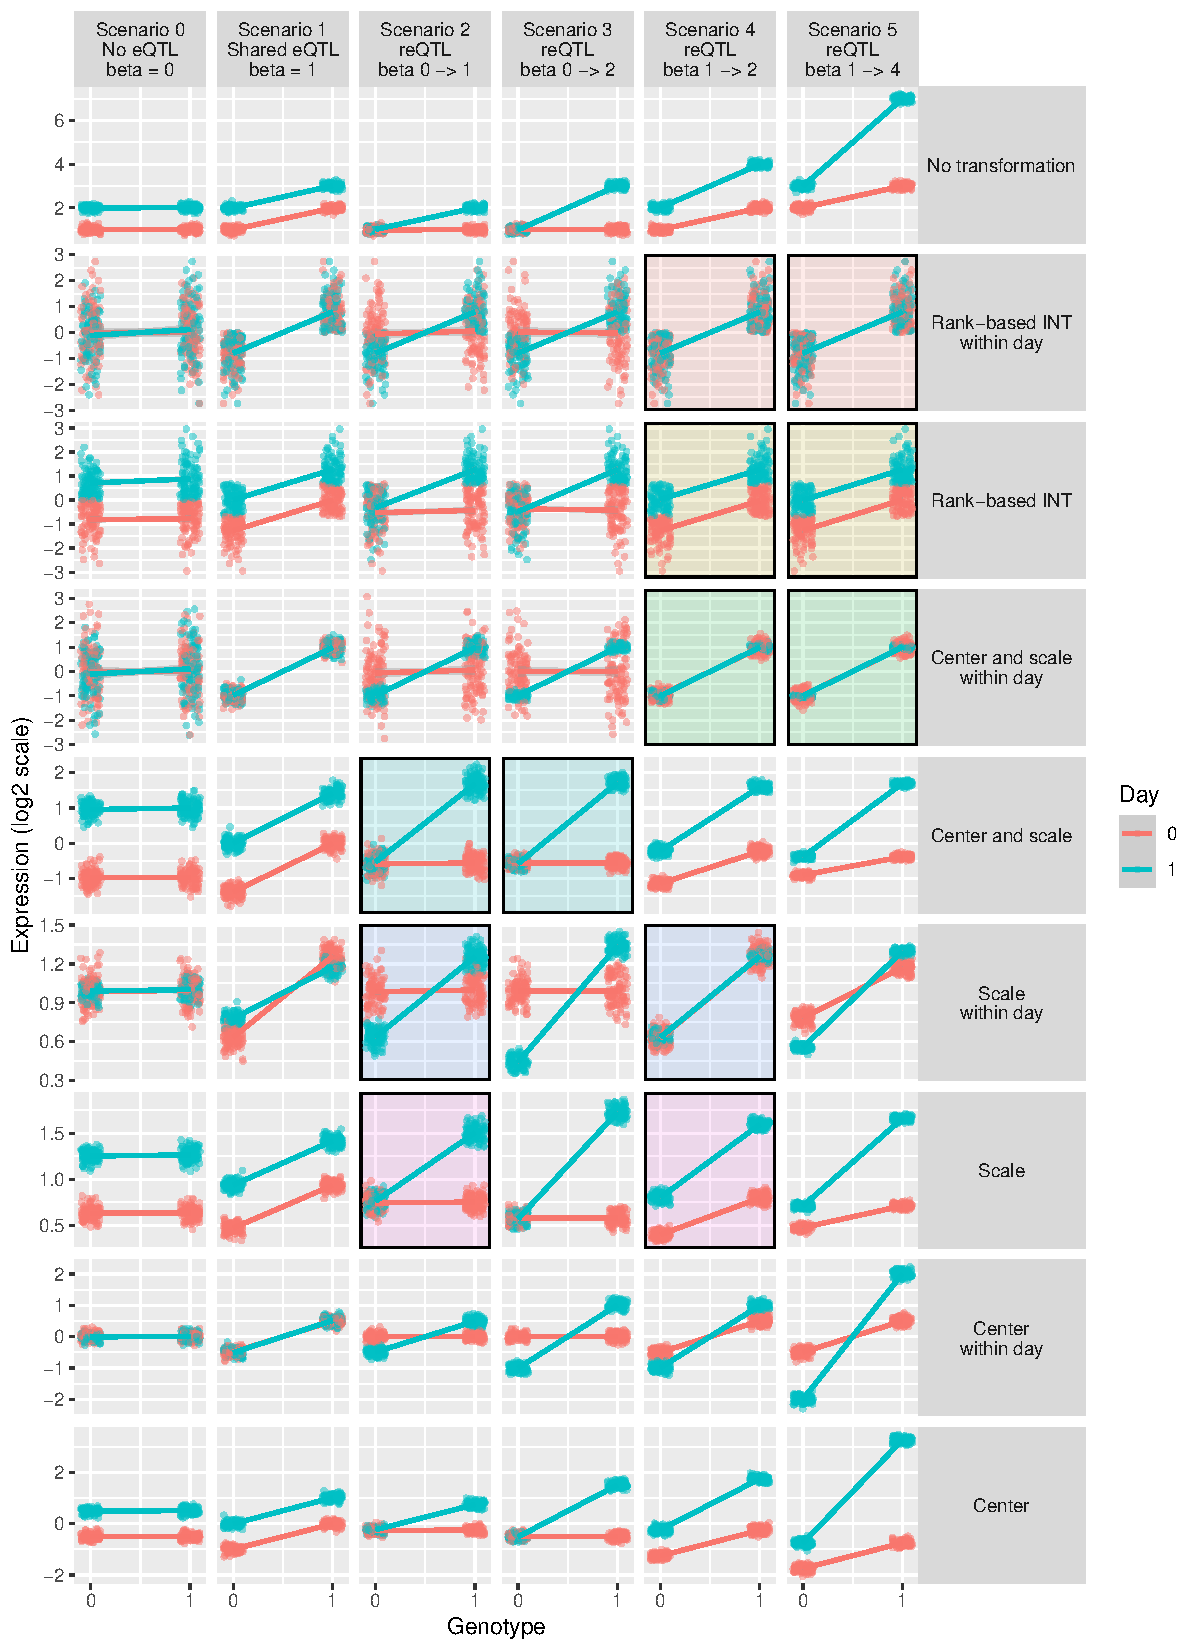
\includegraphics[width=1.0\textwidth,page=1]{mainmatter/figures/chapter_03/simulate_expression_transforms.pdf}
    \caption{
        Simulated log scale expression in two conditions for six genes (columns) representing six different scenarios:
            Scenario 0 has no \gls{eQTL}, 
            scenario 1 is a shared eQTL (beta = 1), 
            scenario 2 is a \gls{reQTL} where beta increases from 0 to 1,
            scenario 3 is a \gls{reQTL} where beta increases from 0 to 2,
            scenario 4 is a \gls{reQTL} where beta increases from 1 to 2,
            and scenario 6 is a \gls{reQTL} where beta increases from 1 to 4.
            Rows represent the effect of different expression transformations across samples, conducted both within condition, and including both conditions.
            Boxed pairs of scenario-transform combinations on each row represent induction of false positives or negatives for reQTLs compared to the ground truth.
            n=100 genotype 1, genotype 2, two dimpoitnes, mean=0, sd=0.1, gaussian noise
            upreg d1 with logfc = 1
    }
    \label{fig:hird_eQTL_expressionTransform_sims}
\end{figure}
% \todo{add sample sizes and model for expression sim}


\subsection{Genotype phasing and imputation}
\label{subsec:hird_reQTL_methods_genotypePhasingAndImputation}

Genotyping and pre-imputation processing are described in \cref{subsec:hird_dge_genotype_data_generation} and \cref{subsec:hird_dge_genotype_preproc}.
% 2.	Online imputation service to phase and impute chr 1-22 and X
% 2.1.	Phase with Eagle v2.4 (version in imputation logs.tar.gz)
% 2.2.	Impute with PBWT 3.1-v3.1-2-gbf6ebe2+htslib-1.3.2-199-gec1d68e-dirty (version in vcf header)
% 2.2.1.	Reference fa is human_g1k_v37.fasta (1000 genomes)
% 2.2.2.	X chrom is done in 3 chunks
% 2.2.2.1.	X:1-2699520: impute against reference resources/refs/imputation/hrc.r1.1/pbwt/HRC.r1-1.GRCh37.chrX_PAR1.shapeit3.mac5.aa.genotypes
% 2.2.2.2.	X:2699521-154931043: impute against reference resources/refs/imputation/hrc.r1.1/pbwt/HRC.r1-1.GRCh37.chrX_nonPAR.shapeit3.mac5.aa.genotypes
% 2.2.2.3.	X:154931044-155270560: impute against reference resources/refs/imputation/hrc.r1.1/pbwt/HRC.r1-1.GRCh37.chrX_PAR2.shapeit3.mac5.aa.genotypes
Prior to imputation, \num{213277} monomorphic variants that provide no information for imputation were removed.
Variant alleles were aligned such that the reference allele matches the GRCh37 reference, and 358 indels were removed, leaving only \glspl{SNP}.
Imputation for the autosomes and X chromosome was conducted using the Sanger Imputation Service\footnote{\url{https://www.sanger.ac.uk/tool/sanger-imputation-service/}}, 
which involved pre-phasing (separate estimation of haplotypes before imputation to improve imputation speed) with EAGLE2 \autocite{loh2016ReferencebasedPhasingUsinga} (v2.4) 
and imputation with PBWT \autocite{durbin2014EfficientHaplotypeMatching} (v3.1) 
against the Haplotype Reference Consortium (r1.1) panel \autocite{mccarthy2016ReferencePanel64}.
Imputed \glspl{SNP} were lifted-over from GRCh37 to GRCh38 coordinates using CrossMap \autocite{zhao2014CrossMapVersatileTool}.
% 4.	Filtering
% 4.1.	BCFTOOLS_INCLUDE="MAF>$MAF_THRESH & F_MISSING<0.05 & FILTER==\"PASS\" & INFO/INFO>0.4"
% 4.2.	Use MAF thresholds 0.05, 0.10, 0.20
Poorly-imputed \glspl{SNP} with imputation information score $\text{INFO} < 0.4$
% or post-imputation missingness $> 5\%$
were removed, leaving \num{40290981} \glspl{SNP} measured for the 169 genotyped individuals.

\subsection{Estimation of kinship matrices}
\label{subsec:hird_reQTL_LDAK}

% 1.	Build GRM using LDAK 5
% 1.1.	Start with pre-imputed genotypes coreex_eQTLflu_20171204.gencall.smajor.impute_sex.qc6
% 1.1.1.	“Estimates of SNP heritability are very sensitive to genotyping errors”, so we can’t use imputed SNPs without filtering for high INFO.
% 1.2.	Prune to MAF 0.05, autosomes only
% 1.3.	Compute LDAK SNP weightings
% 1.4.	Compute kinships for each chromosome
% 1.5.	Join per-chromosome kinships into genome-wide kinships
% 1.5.1.	Use the leave-one-chromosome-out strategy
%
When testing a variant for association using \glspl{LMM}, to avoid loss of power from \enquote{proximal contamination}, the kinship matrix used should not include that variant \autocite{listgarten2012ImprovedLinearMixed}.
% NOTE: new recommendations to leave out only a small window rather than a chromosome \autocite{widmer2015FurtherImprovementsLinear}
A simple way to avoid this is to compute a \gls{LOCO} kinship matrix using all variants except the ones on the tested variant's chromosome \autocite{lippert2011FaSTLinearMixed}.
I estimated kinship in the \gls{HIRD} data from common autosomal variants, using \software{LDAK} (5.0) \autocite{speed2012ImprovedHeritabilityEstimation}, which computes \glspl{SNP}-based kinship matrices, weighting \glspl{SNP} by \gls{LD}.
Filtered, pre-imputation sample genotypes from \cref{subsec:hird_reQTL_methods_genotypePhasingAndImputation} were pruned to $\text{\gls{MAF}} > 0.05$.
A kinship matrix was computed for each autosome, then combined into a single genome-wide matrix using \software{LDAK -{}-join-kins}.
To obtain a \gls{LOCO} kinship matrix for each autosome, each autosome's kinship matrix was then subtracted from this genome-wide matrix (\software{LDAK -{}-sub-grm}).

\subsection{Estimation of cell type abundance from expression}
\label{subsec:hird_reQTL_xCell}

% Full notes about cell type correction pipeline rationale at 2019-10-30 in log
%
\Gls{PBMC} samples are a mixture of immune cells, and a fixed input of RNA extracted from that mixture is used to estimate expression, 
so estimates for genes that have cell type-specific expression depend on the relative abundances of each cell type in each sample.
\textcite{sobolev2016AdjuvantedInfluenzaH1N1Vaccination} showed these abundances shift after Pandemrix vaccination.
As genotype can be assumed to stay constant, it is valid to compare the effect size of genotype on expression between multiple timepoints to call \glspl{reQTL}, 
but changes in cell type abundance complicate this by modifying both expression (cell type-specific expression), 
and the effect of genotype on expression (cell type-specific \gls{eQTL} effects).
Immune cell abundance also varies naturally between healthy individuals \autocite{brodin2015VariationHumanImmune,brodin2017HumanImmuneSystem}, so it is important to model these effects not only post-vaccination, but also at baseline.

Cell type abundance directly measured via \gls{FACS} were only available for a small subset of \gls{HIRD} individuals (\cref{subsec:hird_dge_studyDesign}), so I computed cell type abundance estimates from the expression data as an alternative.
\textit{In silico} estimates have previously been used as covariates in \gls{eQTL} analyses in bulk samples where cell type-specific effects are expected \autocite{westra2015CellSpecificEQTL,zhernakova2017IdentificationContextdependentExpression,davenport2018DiscoveringVivoCytokineeQTL,kim-hellmuth2020CellTypeSpecific}.
As the estimates are based on the expression of multiple genes, is not entirely circular to use them as covariates in this way for per-gene \gls{eQTL} models.
%
% https://github.com/dviraran/xCell
%
% xCell uses the expression levels ranking and not the actual values, thus
% normalization does not have an effect, however normalizing to gene length is
% required.
%
% Importantly, xCell performs best with heterogenous dataset. Thus it is
% recommended to use all data combined in one run, and not break down to pieces
% (especially not cases and control in different runs).  xCell uses the
% variability among the samples for the linear transformation. xCell will only
% function with heterogenous mixtures. If there is no variability between the
% samples, xCell will not identify any signal. As noted above, it is highly
% recommended to use all data combined in one run. Failing to do so will again
% inevitably make xCell's results false.
%
% xCell produces enrichment scores, not percentages. It is not a deconvolution
% method, but an enrichment method. That means that the main usage is for
% comparing across samples, not across cell types. xCell does an attempt to make
% the scores resemble percentages, but it is a hard problem, and is very platform
% and experiment specific. We have made some tests to compare the ability of
% xCell for cross-cell types analysis, and found that it generally performed
% better in that than other methods (on limited and comparable cell types), but
% this type of analysis should be performed carefully.  Regarding this issue,
% scaling the scores by samples is extremely dangerous and will inevitably will
% result in false interpretations.
I selected \software{xCell} \autocite{aran2017XCellDigitallyPortraying}, which previously was shown to outperform other deconvolution methods for cell type-specific \gls{eQTL} mapping in blood \autocite{kim-hellmuth2020CellTypeSpecific}.
\software{xCell} computes enrichment scores based on the expression ranks of approximately \num{10000} signature genes derived from purified cell types,
works for both array and \gls{RNAseq} expression data,
and implements \enquote{spillover compensation} to reduce dependency of estimates between related cell types \autocite{aran2017XCellDigitallyPortraying}.
%
% The spillover compensation step may over compensate, thus it is always better
% to run xCell with a list of cell types that are expected to be in the mixture.
% The names of cell types in this list must be a subset of the cell types that
% are inferred by xCell.
%
\software{xCell} was originally developed for tumour samples, so many of the built-in cell types are not expected to be in \gls{PBMC}.
% See 2019-11-14 log
Reviewing the literature to find which broad classes of peripheral blood cell types are commonly-expected in the \gls{PBMC} compartment \autocite{kleiveland2015PeripheralBloodMononuclear,vanderwijst2018SinglecellRNASequencing,davenport2018DiscoveringVivoCytokineeQTL},
I selected 7/64 of the built-in cell types: CD4\textsuperscript{+} T cells, CD8\textsuperscript{+} T cells, B cells, plasma cells, \gls{NK} cells, monocytes, and \glspl{DC}.
% /nfs/users/nfs_b/bb9/workspace/phd/output/hird/rnaseq/4_de/array/array_data_setup.y.filtered.MaxMean.combat.rds
% and /nfs/users/nfs_b/bb9/workspace/phd/output/hird/rnaseq/4_de/array/array_data_setup.sample.metadata.merged.rds
Array and \gls{RNAseq} data from \cref{subsec:hird_dge_array_preproc} and \cref{subsec:hird_dge_rnaseq_quantAndFilter} were processed through \software{xCell} separately, as different internal parameters are used for each platform.
The large batch effect present in the array expression was first removed using ComBat \autocite{johnson2007AdjustingBatchEffects}.
Finally, enrichment scores were standardised across timepoints, so that a score of zero estimates the average abundance of that cell type across all timepoints.
% (\cref{fig:hird_xCell_scores_heatmap_array} and \cref{fig:hird_xCell_scores_heatmap_rnaseq}).

% \begin{figure}
%     \centering
%     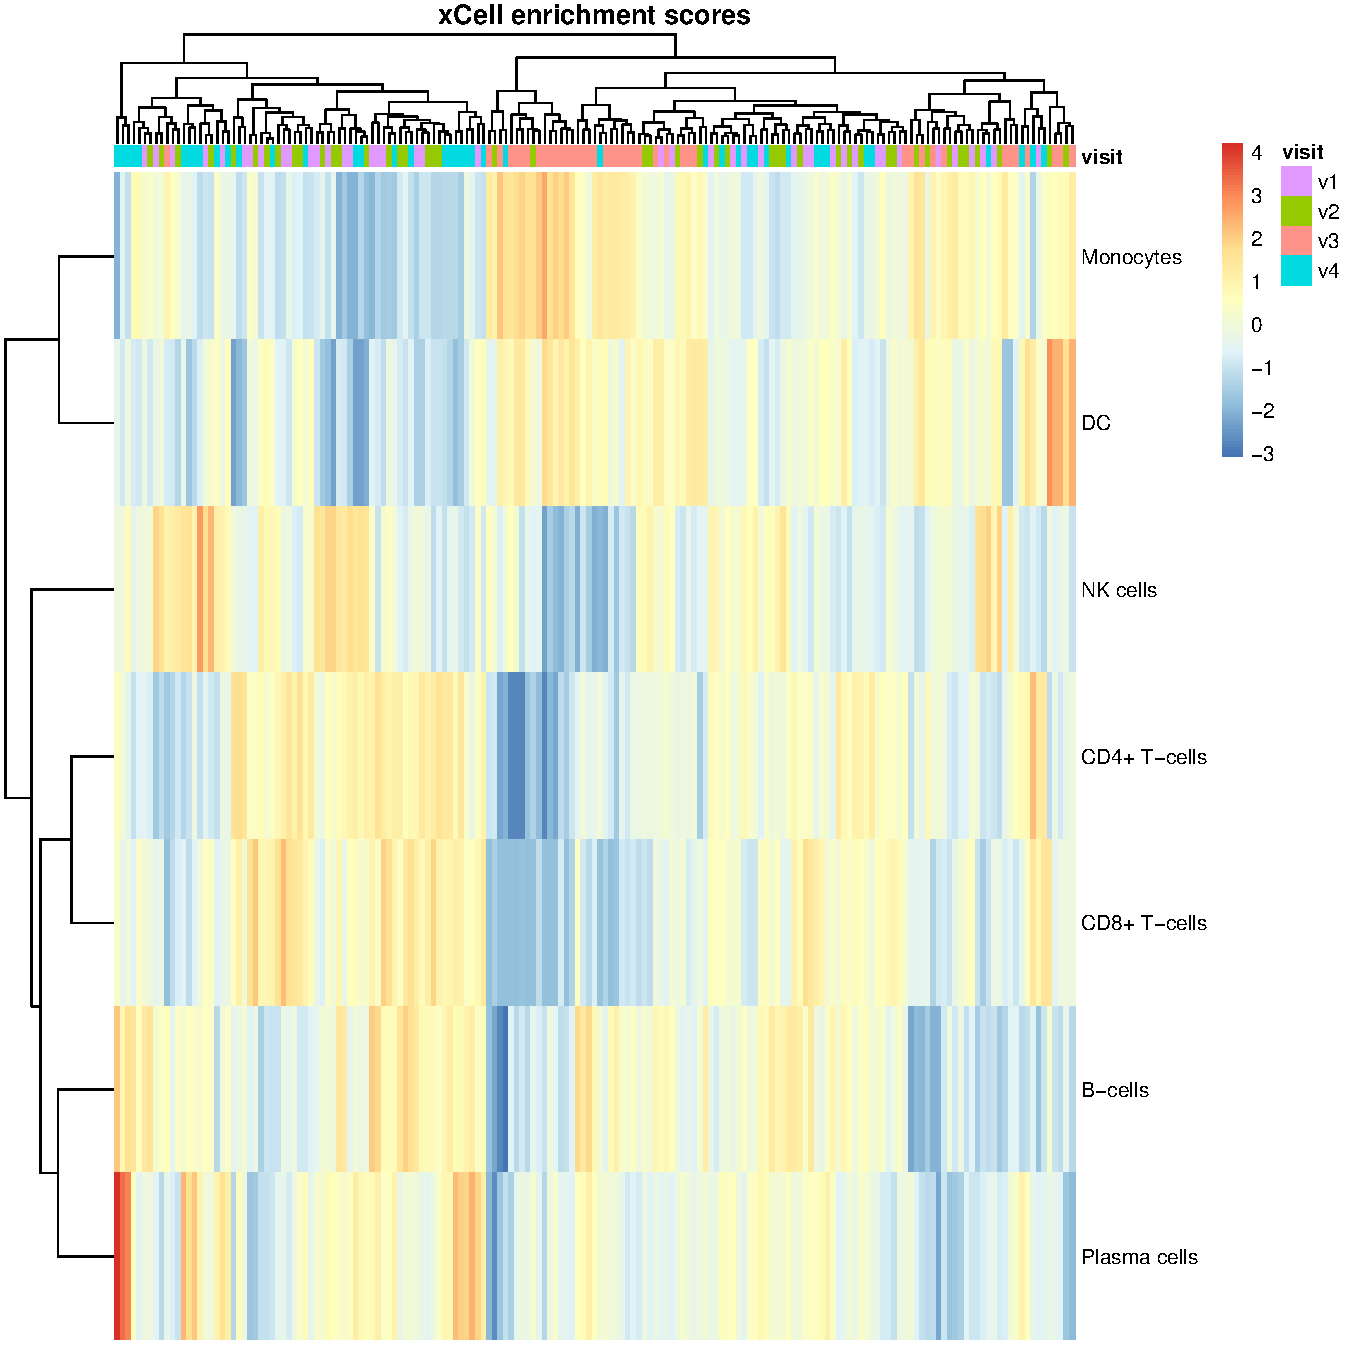
\includegraphics[width=1.0\textwidth,page=1]{mainmatter/figures/chapter_03/get_xCell_estimates.dataset_array.plots.pdf}
%     \caption{Standardised xCell enrichment scores for seven \gls{PBMC} cell types in array samples.}
%     \label{fig:hird_xCell_scores_heatmap_array}
% \end{figure}
%
% \begin{figure}
%     \centering
%     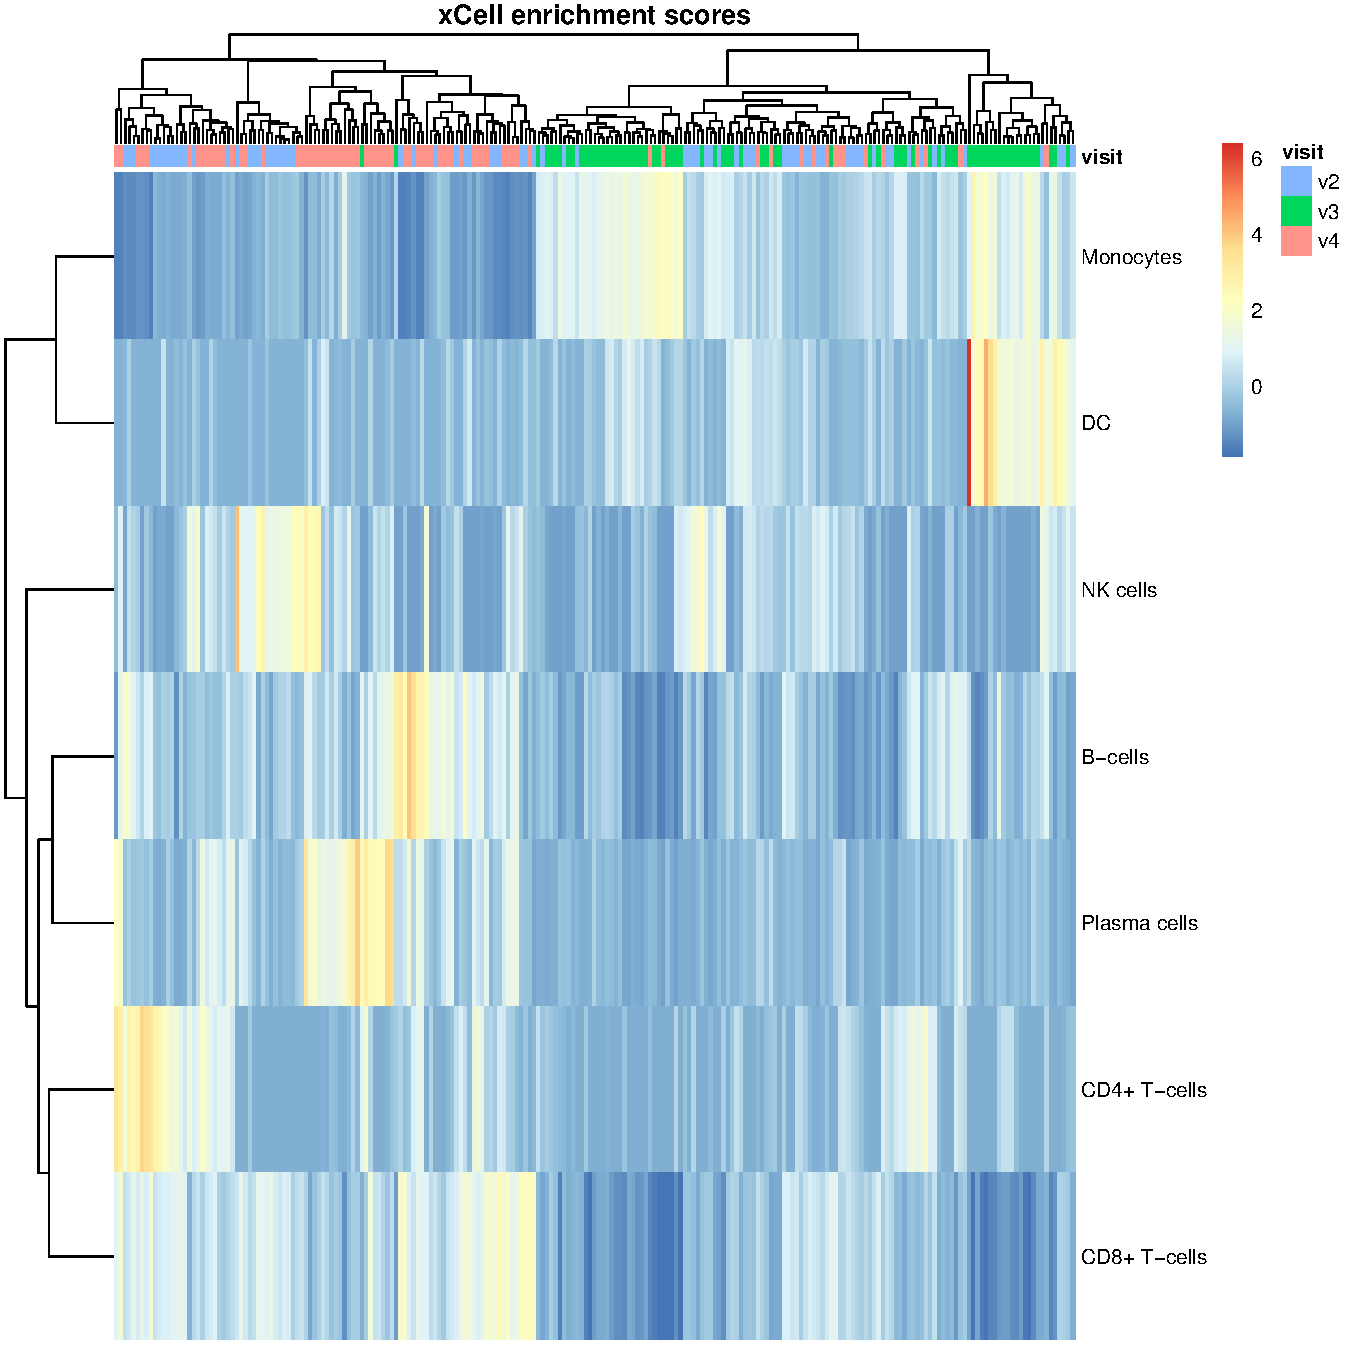
\includegraphics[width=1.0\textwidth,page=1]{mainmatter/figures/chapter_03/get_xCell_estimates.dataset_rnaseq.plots.pdf}
%     \caption{Standardised xCell enrichment scores for seven \gls{PBMC} cell types in \gls{RNAseq} samples.}
%     \label{fig:hird_xCell_scores_heatmap_rnaseq}
% \end{figure}

% xcell estimates not proportions but enrichment scores
As with actual cell type abundances, the enrichment scores are correlated (\cref{fig:hird_xCell_correlationMatrix}).
% NOTE: multicollinearity does not bias the coefficents, but inflates standard errors
Imprecise coefficient estimates due to multicollinearity may be a problem when these scores are used as independent variables in the \gls{eQTL} models% 
\footnote{
    High correlation between predictors is not necessary nor sufficient by itself to induce multicollinearity (predictors being linearly-related), but multiple correlation (how well predictors can be predicted as linear combinations of other predictors) does have an inverse relationship with the standard error of coefficient estimates \autocite{maddala1992IntroductionEconometrics}
}.
% Also see:
% https://stats.stackexchange.com/questions/27300/using-principal-component-analysis-pca-for-feature-selection/27310#27310
To select a subset of cell type scores, I performed a \gls{PCA} of the cell type scores,
separately in array and \gls{RNAseq} datasets (to prevent axes reflecting platform rather than cell type),
% Kaiser Rule
% The more variables that load onto a particular component (i.e., have a high
% correlation with the component), the more important the factor is in
% summarizing the data. An eigenvalue is an index that indicates how good a
% component is as a summary of the data. An eigenvalue of 1.0 means that the
% factor contains the same amount of information as a single variable. [note 1]
the determined the number of \glspl{PC} that exceeded the eigenvalues-greater-than-one rule of thumb \autocite{kanyongo2005InfluenceReliabilityFour}.
In both array and \gls{RNAseq} datasets, the number of components retained was three
The cumulative percentage of variance explained by the top three \glspl{PC} was \SI{81.015345329287}{\percent} and \SI{74.5802450417837}{\percent} in array and \gls{RNAseq} respectively.
Since the \glspl{PC} between the array and \gls{RNAseq} are not directly comparable,
I selected three cell types with high contributions to the top three \glspl{PC} in both datasets:
monocytes, \gls{NK} cells, and plasma cells (\cref{fig:hird_xCell_cos2}).
\textcite{sobolev2016AdjuvantedInfluenzaH1N1Vaccination} reported monocytes and plasma cells to be the cell types with the highest abundance increases at days 1 and 7 respectively.
% The choice to use the actual cell type scores over fitting \glspl{PC} directly as covariates was a sacrifice of orthogonality for interpretability.
Using the actual cell type scores over fitting \glspl{PC} as covariates also provides more interpretable regression coefficients for those terms.

\begin{figure}
    \centering
    \begin{subfigure}[b]{0.65\textwidth}
        \centering
        \includegraphics[width=1.0\textwidth,page=3]{mainmatter/figures/chapter_03/get_xCell_estimates.dataset_array.plots.pdf}
    \end{subfigure}
    \bigskip\vfill
    \begin{subfigure}[b]{0.65\textwidth}
        \centering
        \includegraphics[width=1.0\textwidth,page=3]{mainmatter/figures/chapter_03/get_xCell_estimates.dataset_rnaseq.plots.pdf}
    \end{subfigure}
    \caption{
        \textbf{Correlation matrix of standarised xCell cell type enrichment scores in each dataset.}
        Rows and columns are hierarchically-clustered.
    }
    \label{fig:hird_xCell_correlationMatrix}
\end{figure}

% See:
% https://stats.stackexchange.com/questions/119746/what-is-the-proper-association-measure-of-a-variable-with-a-pca-component-on-a
%
% https://stats.stackexchange.com/questions/495342/pca-and-variable-contributions-to-first-n-dimensions
% If you have a "PCA" object constructed using FactoMineR::PCA, then variable contribution values are stored in the $var$contrib slot of your object. The contribution is a scaled version of the squared correlation between variables and component axes (or the cosine, from a geometrical point of view)
%
% var$contrib: contains the contributions (in percentage) of the variables to the
% principal components. The contribution of a variable (var) to a given principal
% component is (in percentage) : (var.cos2 * 100) / (total cos2 of the
% component).
\begin{figure}
    \centering
    \begin{subfigure}[b]{0.65\textwidth}
        \centering
        \includegraphics[width=1.0\textwidth,page=10]{mainmatter/figures/chapter_03/get_xCell_estimates.dataset_array.plots.pdf}
    \end{subfigure}
    \bigskip\vfill
    \begin{subfigure}[b]{0.65\textwidth}
        \centering
        \includegraphics[width=1.0\textwidth,page=10]{mainmatter/figures/chapter_03/get_xCell_estimates.dataset_rnaseq.plots.pdf}
    \end{subfigure}
    \caption{
        \textbf{
            Contribution of each cell type score to each \gls{PC} dimension after \gls{PCA} of standarised xCell cell type enrichment scores. 
        }
        Contribution is calculated as the squared correlation between a variable and a \gls{PC} (cos2), 
        scaled to the sum of cos2 for all variables with \gls{PC}.
        High contributions indicate variables that are correlated with the \gls{PC}.
    }
    \label{fig:hird_xCell_cos2}
\end{figure}

Scores were validated against \gls{FACS} measurements from \textcite{sobolev2016AdjuvantedInfluenzaH1N1Vaccination} in the subset of \textapprox{40} individuals that had both expression and \gls{FACS} data.
Depending on each \gls{FACS} panel's gating strategy for each cell subset, the data were in units of either absolute counts, or percentage of the previously gated population.
Values were normalised by rank-based \gls{INT} within each panel and cell subset (\autocite{astle2016AllelicLandscapeHuman} takes a similar approach for cell abundance data using a quantile-based \gls{INT}).
% RANK INT also used in phenome scan PHEASANT https://www.biorxiv.org/content/biorxiv/early/2017/02/26/111500.full.pdf
%
% missForest is a nonparametric imputation method for basically any kind of data.
% It can cope with mixed-type of variables, nonlinear relations, complex
% interactions and high dimensionality(p>>n). It only requires the observation
% (i.e. the rows of the data frame supplied to the function) to be pairwise independent.
Missing values were then imputed with MissForest \autocite{stekhoven2012MissForestNonparametricMissing}, a random forest imputation method suitable for high-dimensional mixed-type data where $p \gg n$.
An initial guess for missing values is established using mean- or mode-imputation, then a random forest is trained on the observed part of the data and used to predict and update the values of the missing part.
The process repeats iteratively until convergence.
% NOTE:
% Why impute for cell counts but not for expression data?
% - expression matrices are mostly complete, and we only exclude genes based on low expression in RNAseq
% - we cannot drop whole FACS panels so easily like we can drop genes

Although the increases in xCell score for monocytes at day 1 and plasma cells at day 7 do reflect the increases in these cell types observed by \textcite{sobolev2016AdjuvantedInfluenzaH1N1Vaccination}, overall correlation between xCell and \gls{FACS} was poor (\cref{fig:hird_xCell_vs_FACS}).
Substantial discrepancy was expected, as the cell types as defined in the xCell signatures do not directly correspond to the combinations of surface markers used for \gls{FACS}; the comparison is against the closest match.
The \gls{FACS} gating strategy also meant that for some cell populations, the only available \gls{FACS} measure was a proportion of the previously gated population,
whereas xCell attempts to estimate scores that represent enrichments in the whole mixture.
The accuracy of the built-in signatures may also be lower when applied to the expression matrix for a stimulated state,
and an enrichment-based method can not distinguish per-cell differential expression of signature genes from changes in cell abundance.
A custom signature matrix can be used for xCell, perhaps drawn from an independent study with similar stimulation conditions as \gls{HIRD} such as \textcite{franco2013IntegrativeGenomicAnalysis}, but this would not solve the issue of coupled differential expression and cell abundance.
Weighing the downsides of having imperfect estimates of cell type abundance against the downsides of not accounting for abundance, or excluding samples without \gls{FACS} measures, I chose to continue the analysis using the xCell scores.
These scores can distinguish large changes in cell abundances between days, but may not be reliable for distinguishing small differences in abundance between individuals with a timepoint. 

\begin{figure}
    \centering
    \begin{subfigure}[b]{0.43\textwidth}
        \centering
        \includegraphics[width=1.0\textwidth,page=6]{mainmatter/figures/chapter_03/validate_xCell_estimates.cell_type_pairs.pdf}
        \caption{Monocytes.}
    \end{subfigure}
    \bigskip\vfill
    \begin{subfigure}[b]{0.43\textwidth}
        \centering
        \includegraphics[width=1.0\textwidth,page=3]{mainmatter/figures/chapter_03/validate_xCell_estimates.cell_type_pairs.pdf}
        \caption{\gls{NK} cells.}
    \end{subfigure}
    \bigskip\vfill
    \begin{subfigure}[b]{0.43\textwidth}
        \centering
        \includegraphics[width=1.0\textwidth,page=2]{mainmatter/figures/chapter_03/validate_xCell_estimates.cell_type_pairs.pdf}
        \caption{Plasma cells.}
    \end{subfigure}
    \caption{
        \textbf{Comparison of standardised xCell scores for monocytes, \gls{NK} cells and plasma cells with normalised \gls{HIRD} \gls{FACS} measurements.}
        The comparisons are against the most comparable measurements from the \gls{FACS} data of \textcite{sobolev2016AdjuvantedInfluenzaH1N1Vaccination}: 
        CD14+ monocyte count,
        CD56+ NK cells count,
        and the proportion of CD19+ B cells that were CD19+CD27+CD24hiCD38hi plasma cells.
        Missing \gls{FACS} values were imputed with MissForest after rank-based \gls{INT} transformation.
    }
    \label{fig:hird_xCell_vs_FACS}
\end{figure}

\subsection{Finding unmeasured covariates using factor analysis}

% If RANKINT, why RANKINT before PEER?
%
% Are your covariates under control? How normalization can re-introduce covariate effects
% https://www.ncbi.nlm.nih.gov/pubmed/29706643
% "Many statistical tests rely on the assumption that the residuals of a model are normally distributed [1]. In genetic analyses of complex traits, the normality of residuals is largely determined by the normality of the dependent variable (phenotype) due to the very small effect size of individual genetic variants [2]. However, many traits do not follow a normal distribution."
% "applying rank-based INT to the dependent variable residuals after regressing out covariates re-introduces a linear correlation between the dependent variable and covariates, increasing type-I errors and reducing power."

% 2.	Infer global confounders by detecting hidden factors affecting expression with PEER
% 2.1.	“batch effects and other global confounders reduce the power to find expression quantitative trait loci”
% 2.1.1.	“We assume that these variables have a broad influence, and thus each of them has an effect size for every gene.”
% 2.1.2.	“The learned variables can be constrained to affect known sets of genes via a prior connectivity matrix. By default, with no prior connectivity given, they are assumed to be global and to affect large fractions of all genes“
% 2.1.3.	Note that due to this assumption: “If large trans hotspots are dominating, associations may get erroneously explained away as confounding factors”
% 2.2.	Round input expression to integer counts
% 2.2.1.	Input is y: the scaledTPM (TPM's scaled up to library size) from tximport.
% 2.3.	Normalise for library size and variance stabilize with varianceStabilizingTransformation from DESeq2 (recommended in PEER paper)
% 2.3.1.	Vst is like a souped up log: “In all cases, the transformation is scaled such that for large counts, it becomes asymptotically (for large values) equal to the logarithm to base 2 of normalized counts.”
% 2.3.2.	Note we cannot use voom-ed expressions from the DGE pipeline, as there are some samples missing due to lack of Ab titre data
% 2.3.3.	Do not blind the transformation to experimental design matrix: “If many of genes have large differences in counts due to the experimental design, it is important to set blind=FALSE for downstream analysis.”
% 2.3.4.	Here we use a simple design matrix of groups defined by all combos of day x R/NR
% 2.4.	Run PEER by timepoint
% 2.4.1.	Match GTeX pipeline: https://github.com/broadinstitute/gtex-pipeline/tree/63b13b8ced25cf8ab8e7a26f40a495e523630a9b/qtl , with some modifications.
% 2.4.1.1.	Note this pipeline uses quantile normalized, rank INT transformed expression, as PEER input
% 2.4.2.	Quantile normalize the samples with preprocessCore::normalize.quantiles
% 2.4.2.1.	Causes the expressions of the samples to have the same empirical distribution
% 2.4.2.2.	i.e. the the highest expression in each sample is set to the mean of the highest values of all samples, and in the case of no tied values, each sample’s expressions becomes a permutation of each other sample’s
% 2.4.3.	Standardize expression of each gene with Rank-Based Inverse Normal Transformation
% 2.4.3.1.	i.e. rank the expressions of a gene, then replace with values from the standard normal e.g. > rank.based.INT(1:5, c=3/8): [1] -1.1797611 -0.4972006  0.0000000  0.4972006  1.1797611
% 2.4.4.	Setup and run PEER
% 2.4.4.1.	Allow up to 10k iterations, start with n.samples/4 PEER factors
% 2.4.4.2.	One can include known covariates. We don’t, as it causes weird things like PEER factors not being sorted in descending relevance
% 2.4.4.2.1.	~ 1 + batch + rna.conc + Gender + Age.at.vaccination..years. + PC1.imputed + PC2.imputed + PC3.imputed + PC4.imputed
% 2.4.4.2.2.	Note this includes an intercept that represents the mean expression
%
% Also interesting:
% PANAMA/LIMMI, by PEER authors
% Detecting regulatory gene–environment interactions with unmeasured environmental factors
%
Apart from cell type abundance, a myriad of other unmeasured variables contribute to expression variation.
Hidden determinants of expression variation were learnt using \software{PEER} \autocite{stegle2012UsingProbabilisticEstimation}.
As suggested by \textcite{stegle2012UsingProbabilisticEstimation}, I used \software{DESeq2::vst} to perform between-sample normalisation and variance stabilisation on \gls{RNAseq} count data%
\footnote{
    The count data were taken from \cref{subsec:hird_dge_rnaseq_quantAndFilter} before \gls{TMM} normalisation and voom transformation,
    as PEER cannot use the weights output by those methods for between-sample normalisation and variance stabilisation as limma can.
}.
ComBat was applied to first merge array and \gls{RNAseq} data into a single log scale expression matrix per timepoint, treating the largest global effects on expression---the two array batches and three \gls{RNAseq} library prep pools (\cref{fig:hird_expression_pcs})---as known batch effects.
% (e.g., by introducing principal components of the genotype data), is not included in the model, and it may be recapitulated in the inferred factors.
Given selected known covariates (intercept, sex, four genotype \glspl{PC} from \cref{subsec:hird_dge_genotype_pc} representing ancestry, and the three xCell scores estimated above),
% TODO: sole motivation here is efficiency. not so much confounding. PEER finds factors that explain var. so given factors are included for the sake of downstream modelling interest
% this is also the primary motivation behind recommendation of including prognostic covariates in RCTs \url{https://trialsjournal.biomedcentral.com/articles/10.1186/1745-6215-15-139}
PEER was used to estimate additional hidden factors that explain variation in expression matrix.
% TODO: what might they be?
% technical
%  Flow Cell
%  Lane
%  Adaptors
%  Library prep reagents
%  Same instrument
%  People!
%  Day
%  RNA extraction/purification
% see https://academic.oup.com/bib/article/12/3/280/258477#3083943
% or biological, like cell counts
Factors are assumed to be unmeasured covariates that have global effects on a large fraction of genes, 
whereas a cis-\gls{eQTL} will typically only have local effects, so including factors as covariates should not introduce dependence with the genotype term,
but should soak up some of residual variation, improving power to detect cis-\glspl{eQTL}.
The analysis was run per timepoint, otherwise global changes in expression between timepoints induced by the vaccine would be recapitulated as factors.
% TODO: not like PCs: not orthogonal or uncorrelated
% TODO: add auto relevance ,
% TODO: do not keep explaining more var. var of factors themselves declines
% and no guarantee of decreasing order when known

Correlating the estimated factors to a larger set of known covariates reveals many correlations with xCell estimates, indicating that cell type abundance does indeed have substantial global effects on the expression matrix.
% TODO: and we get more!
There is little correlation with known array or \gls{RNAseq} batch effects, indicating ComBat did an adequate job of removing batch- and platform-dependent global effects on expression (\cref{fig:hird_peer_corMatrix_v2_mega}).
Note that I did not leave this adjustment for PEER to perform, as ComBat estimates centering and scaling factors per gene to adjust for batch effects, whereas the use of PEER factors represent a mean-only adjustment
Given the severity of the batch effect in this dataset, especially between platforms, mean-only adjustment may be insufficient\autocite{zhang2018AlternativeEmpiricalBayes}.

\begin{figure}
    \centering
    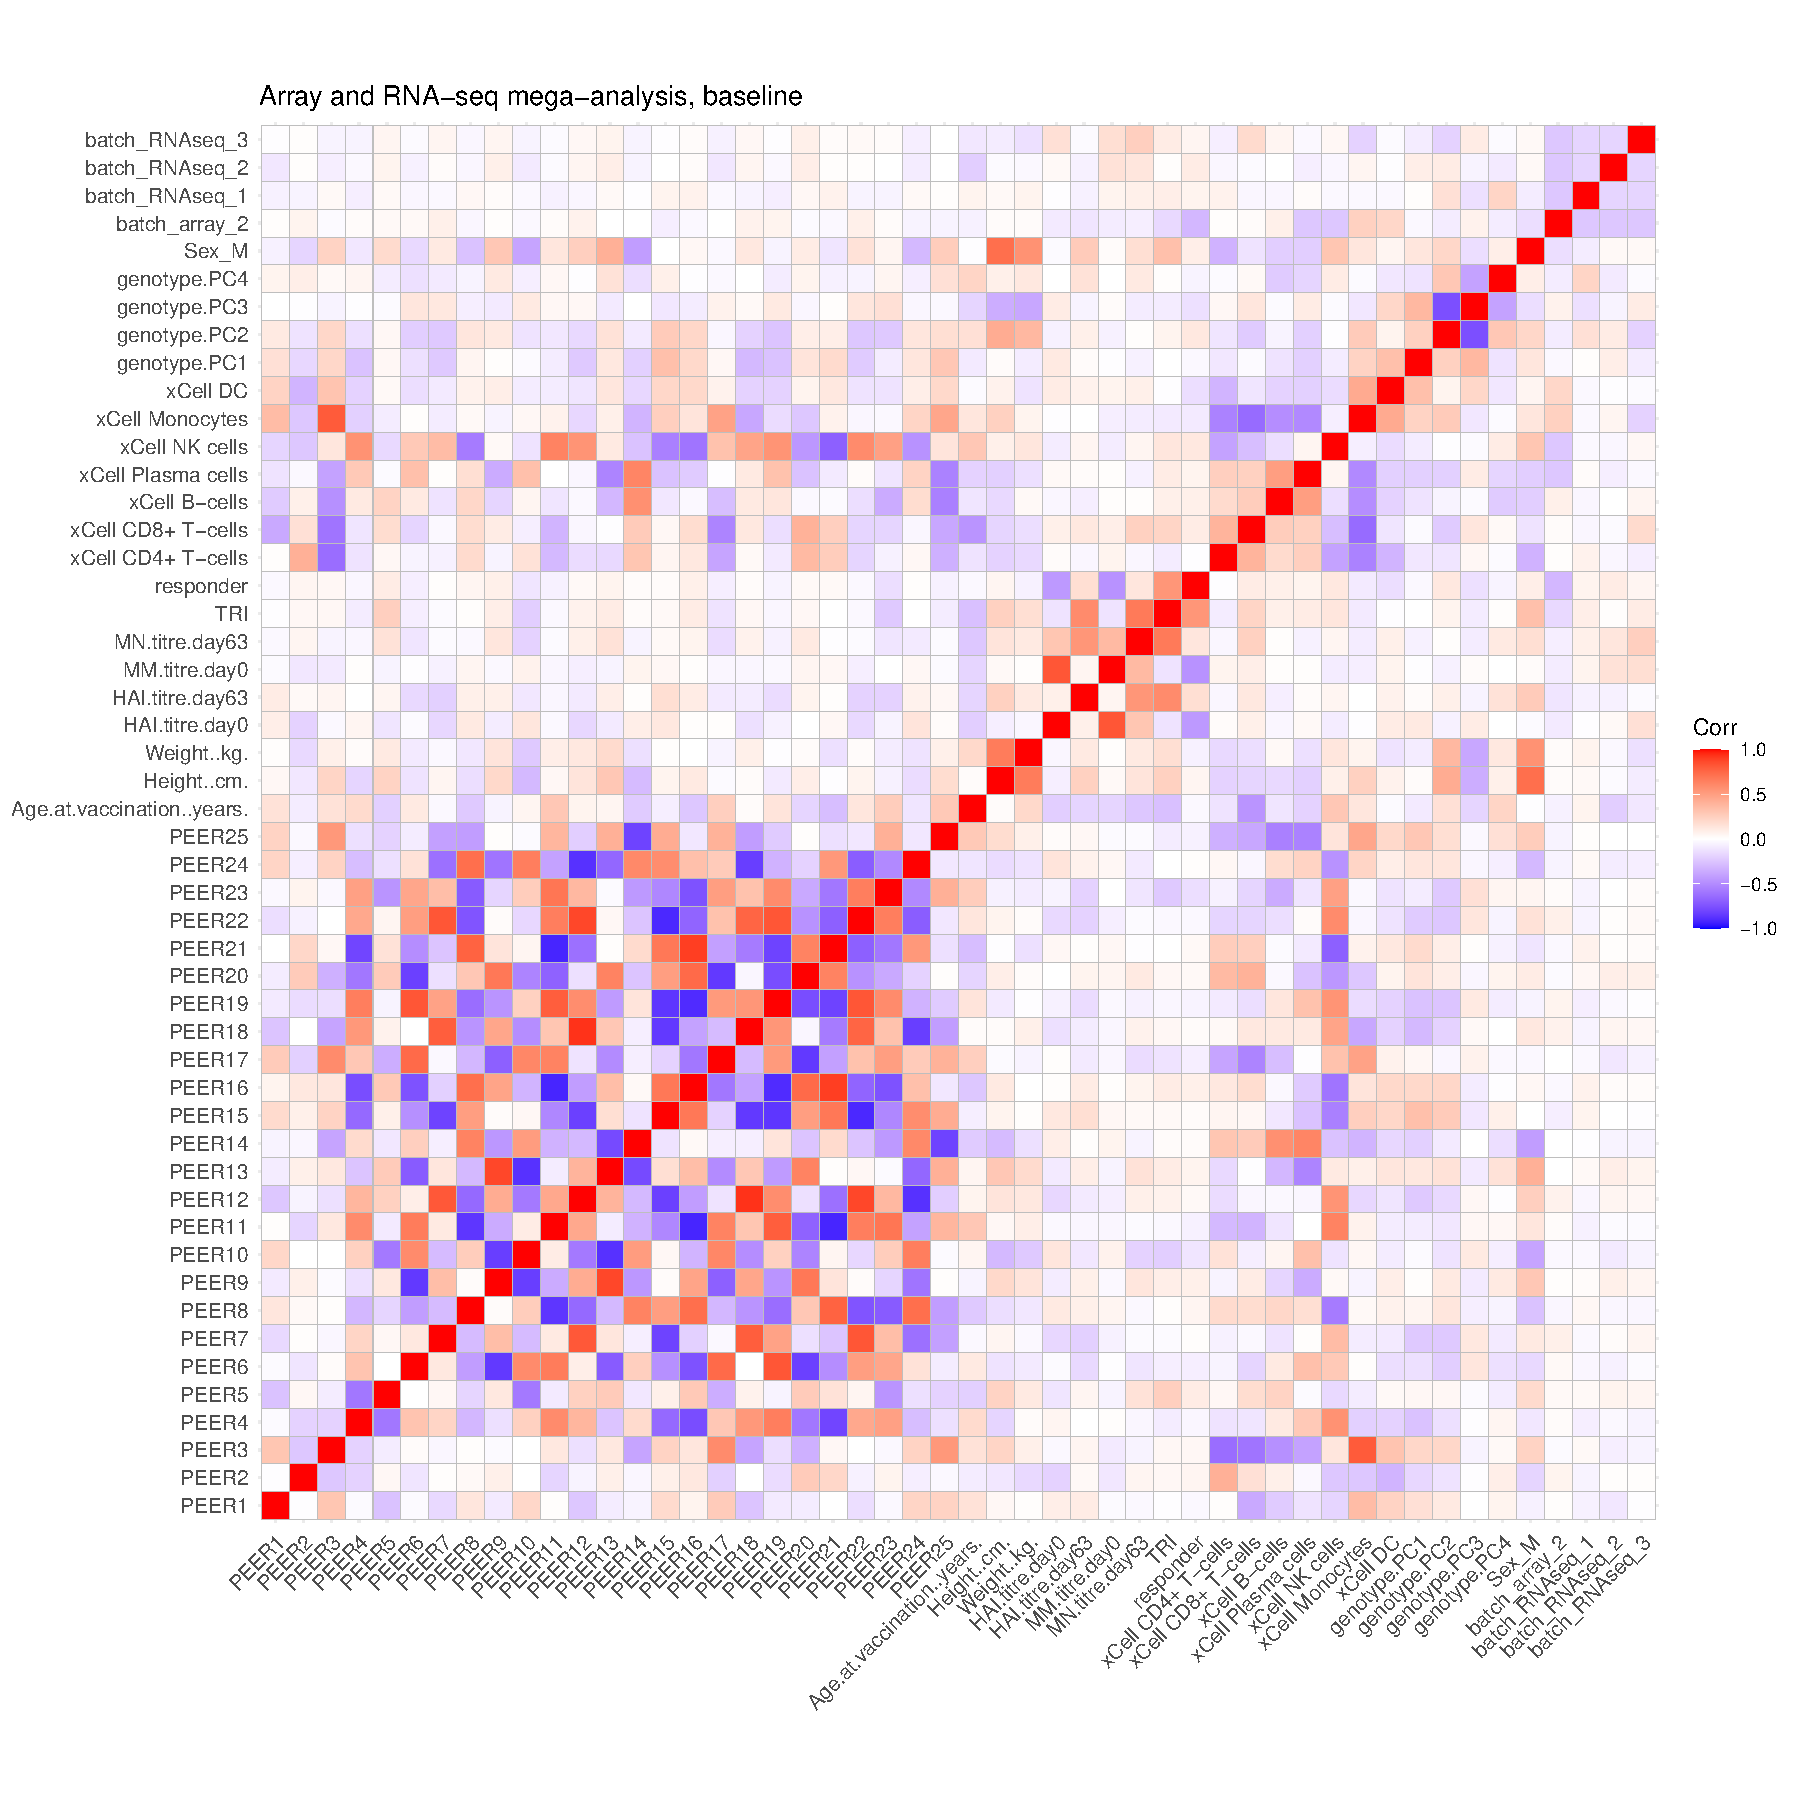
\includegraphics[width=1.0\textwidth,page=1]{mainmatter/figures/chapter_03/peer_plotting.mega_v2.pdf}
    \caption{Correlation of PEER factors to known factors and other possible covariates. Note that PEER factors are not constrained to be orthogonal, so correlations to known factors are expected.}
    \label{fig:hird_peer_corMatrix_v2_mega}
\end{figure}
\todo{remake this with only top k factors, and prune the possible covariates}

% TODO: if we use PEER, why also use LMM?
% PEER only ajusts for large sclae e.g. YRI vs EU
% not finer scale e.g within EU
% \autocite{brown2018ExpressionReflectsPopulation}
% Interestingly, we found that using PEER rather than regression for batch correction also
% removed the separation between the YRI and EUR individuals, while leaving the structure
% within the EUR populations in tact (Fig 5A).

\subsection{\glsfmtshort{eQTL} mapping per timepoint}

% 2.5.	Preprocess genotypes for limix
% 2.5.1.	Convert MAF filtered VCF -> 012 -> hdf5 format
% 2.5.1.1.	Do this for both strict 012 and continuous dosages
% 2.5.2.	Also convert 012 -> matrix eqtl SNP matrix format
% 2.5.2.1.	For eigenMT
% 2.5.3.	Parse out snpinfo and snplocs from VCFs
% 2.5.3.1.	Snpinfo for snp ids, for limix
% 2.5.3.2.	Snplocs for snp positions, and eigenMT
% 2.6.	Map eQTLs using limix 2.0, per timepoint
% 2.6.1.	Map cis-eQTLs within +- 1Mb of the gene start
% 2.6.1.1.	Phenotypes: per timepoint normalised input.expr from PEER script
% 2.6.1.2.	Covariates: sex, batch, 4 genotype PCs, 4 PEER factors
% 2.6.1.3.	Genotypes: MAF > 0.10 (in whole 169 individuals)
% 2.6.1.4.	Kinship: from LDAK, leave-one-chrom-out
% 2.6.2.	Output results in matrix eqtl-like output format
%
I mapped \glspl{eQTL} within each timepoint using \software{LIMIX} \autocite{lippert2014LIMIXGeneticAnalysis}, which implements univariate and multivariate \glspl{LMM} with one or more random effects.
Imputed genotype probabilities were converted to continuous alternate allele dosages using bcftools (1.7-1-ge07034a).
Variants with sample $\text{\gls{AC}} < 15$ within each timepoint were excluded.
% TODO:
% per timepoint weakness here is that filtering MAF when unequal sizes restricts assessible results to lowest n
% but, due to tagging, not all hope is lost
\todo{add approximate MAFs, then cite hierarch paper}
% As is standard for imputation, we excluded all X-linked SNPs for the
% following reasons: (i) the X chromosome has to be treated differently from
% the autosomes; (ii) it cannot be predicted which allele is active on the X
% chromosome, (iii) testing males separately from females results in different
% sample sizes and power. Imputation of SNPs in the HapMap CEU population was
% performed using either MACH46 or IMPUTE47. All SNPs with a MAF <0.01 were
% excluded from analysis. In total, up to 2.11 million genotyped or imputed
% SNPs were analyzed.
% For example, an allele count of 1 in a female indi-cates a heterozygote
% genotype (one reference and onealternative allele), while a count of 1 in a
% male means only alternative allele exists and may cause more pro-found
% effects. The variance of the genetic effect may also differ between genders.
%
% X chromosome variants were excluded, as the number of copies differ between males and females, and X-inactivation makes it difficult to determine the active allele \url{https://www.nature.com/articles/ng.467},
% so sex-specific methods are required \url{http://www.biomedcentral.com/1471-2105/15/392}.
% \todo{add note on treating x chrom variants with caution}

At each of 13570 genes, at all cis-variants within within $\pm \SI{1}{\mega\bp}$ of the gene \gls{TSS}, I fit the following model to map \gls{eQTL}:
% TODO
% Ensembl GENESEQSTART if fwd strand, otherwise GENESEQEND
 % Like all Ensembl features the start of an exon is always less than or equal to the end of the exon, regardless of the strand it is on. The start of the transcript is the start of the first exon of a transcript on the forward strand or the end of the last exon of a transcript on the reverse strand. The start and end of a gene are defined to be the lowest start value of its transcripts and the highest end value respectively.
\begin{equation}
\begin{split}
Y = 1 + sex + \sum_{i=1}^{4}{PC_i} + \sum_{}^{3}{xCell} + \sum_{i=1}^{k}{PC_i} + \beta G + \mathbf{u} + \epsilon
\end{split}
\label{eq:hird_reQTL_limix_model}
\end{equation}
% TODO: check mathbf for vector notation, add timepoint subscript
where the \gls{eQTL} effect size of interest is the slope of the genotype fixed effect $\beta$, the average additive effect of the alternate allele \autocite{visscher2019Fisher1918Paper};
and $\mathbf{u} \sim N(0, \sigma_g^2 K)$ is a random effect with zero mean and covariance matrix proportional to the \gls{LOCO} kinship matrix.
For chromosome X variants, no \gls{LOCO} matrix is available from LDAK, so the matrix for chromosome 1 was used.
% The LMM requires a kinship matrix to scale the covariance matrix of the random effect mean zero and an unknown variance.
% In the past, the only available measure of genetic similarity was a kinship coefficient computed as a probability of identity by descent in a pedigree, and so a single random effect term sufficed to model genome-wide additive effects. Nowadays genetic similarity can be measured directly, and in many different ways, from genome-wide SNP data.
% GRM is : "consists of average allelic correlations across the SNPs (adjusted for LD and genotype certainty)" https://www.nature.com/articles/ng.3865?proof=true
% By default, LDAK scales kinships to have mean zero and average diagonalone
% \todo{note stacking of kinship for day -7 repeated measures}

PEER factors are automatically weighted such that the variance of factors tends to zero as more factors are estimated, 
hence continuing to add more and more factors as covariates will not continue to improve \gls{eQTL} detection power, and eventually the model degrees of freedom will be depleted.
To optimise k, the number of factors to include as covariates%
\footnote{I avoid the commonly-performed two-stage approach of treating PEER residuals as expression phenotypes, as the degrees of freedom seen downstream will be incorrect, which can have a substantial effect on estimates at this modest sample size.}, 
% Also see \autocite{demissie2011BiasDueTwostage} % holmes2019ProblemsInterpretingUsing
Per-timepoint \gls{eQTL} mapping was performed in chromosome 1, iteratively increasing the number of factors until the number of \glspl{eQTL} detected plateaus.
I settled on a final choice of $k=10$ factors for pre-vaccination, 5 factors for day 1, and 5 factors for day 7 (\cref{fig:hird_neGenesvsPeerK}).
\todo{i leave the pcs in to guard against unusually differentiated between pop markers, where random effect alone may not be enough \autocite{price2010NewApproachesPopulation}, \url{https://www.nature.com/articles/srep06874}}

\begin{figure}
    \centering
    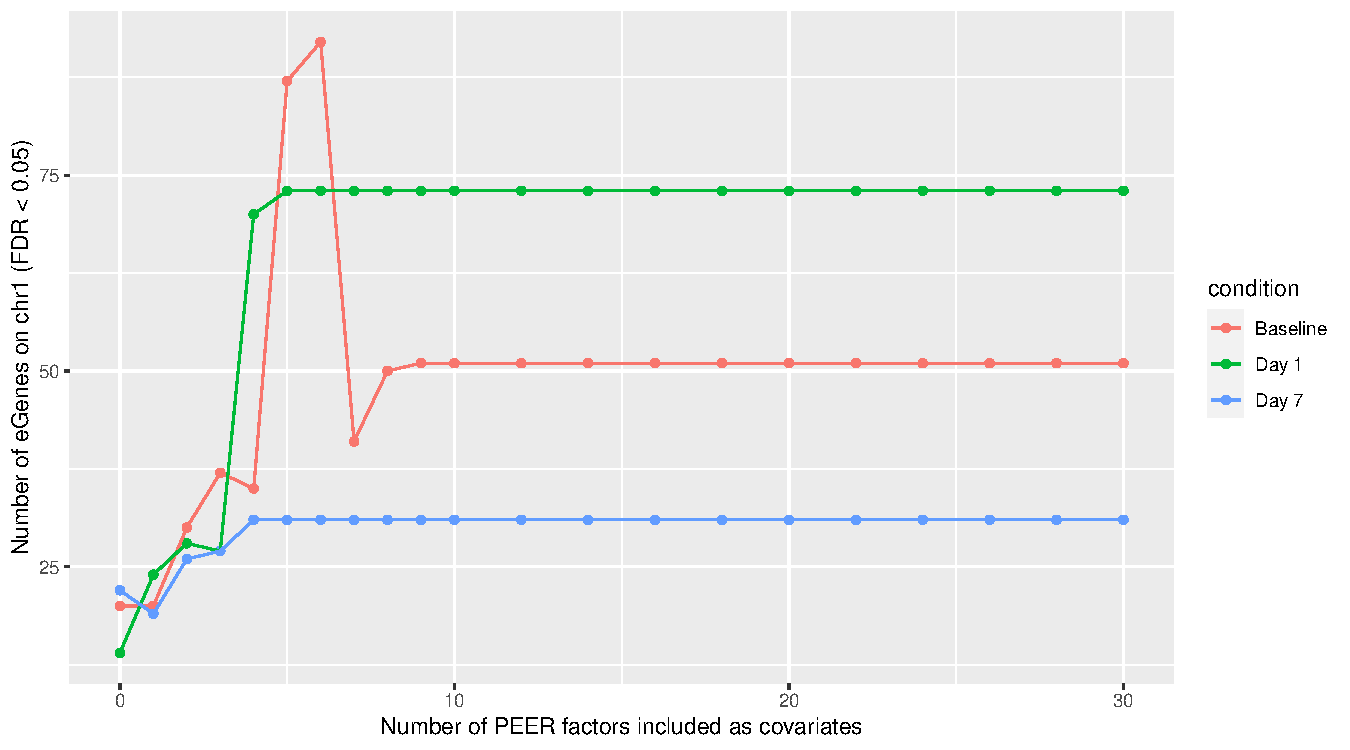
\includegraphics[width=1.0\textwidth,page=1]{mainmatter/figures/chapter_03/count_eGenes.signif_eGenes_vs_PEER_n.dataset_mega.chr_chr1.pdf}
    \caption{Number of significant eGenes detected on chromosome 1 (hierarchical Bonferroni-\gls{BH}\autocite{huang2018PowerFalseDiscovery} FDR < 0.05) as a function of the number of PEER factors included as covariates k.}
    \label{fig:hird_neGenesvsPeerK}
\end{figure}

\subsection{Joint \glsfmtshort{eQTL} analysis across timepoints}

% 2.10.	mashr
% 2.10.1.	Apply mashr to per-day meta-analysis beta/beta_ste results
Joint analysis was conducted with \software{mashr}\autocite{urbut2018FlexibleStatisticalMethods}, at 40197618 gene-variant pairs (mean of \num[round-mode=places,round-precision=0]{2962.24156227} tests per gene) for which summary statistics from within timepoint mapping were available in all three timepoint conditions.
% \todo{recheck if did I do a SNPs only filter} NOTE: yes i did
The mashr model incorporates multiple canonical (the identity matrix etc.) and data-driven covariance matrices to represent patterns of effects across conditions (in this case, $3 x 3$ matrices).
Data-driven covariance matrices are derived by dimension reduction of a strong subset of tests likely to have an effect in at least one condition.
I took the most significant variant per gene per condition, 
which ensures strong condition-specific effects are included,
% (\cref{fig:hird_mashr_strongSubset_Z_mega}),
then further filtered to only nominally significant tests, resulting in a strong subset of 45962 tests.

% \begin{figure}
%     \centering
%     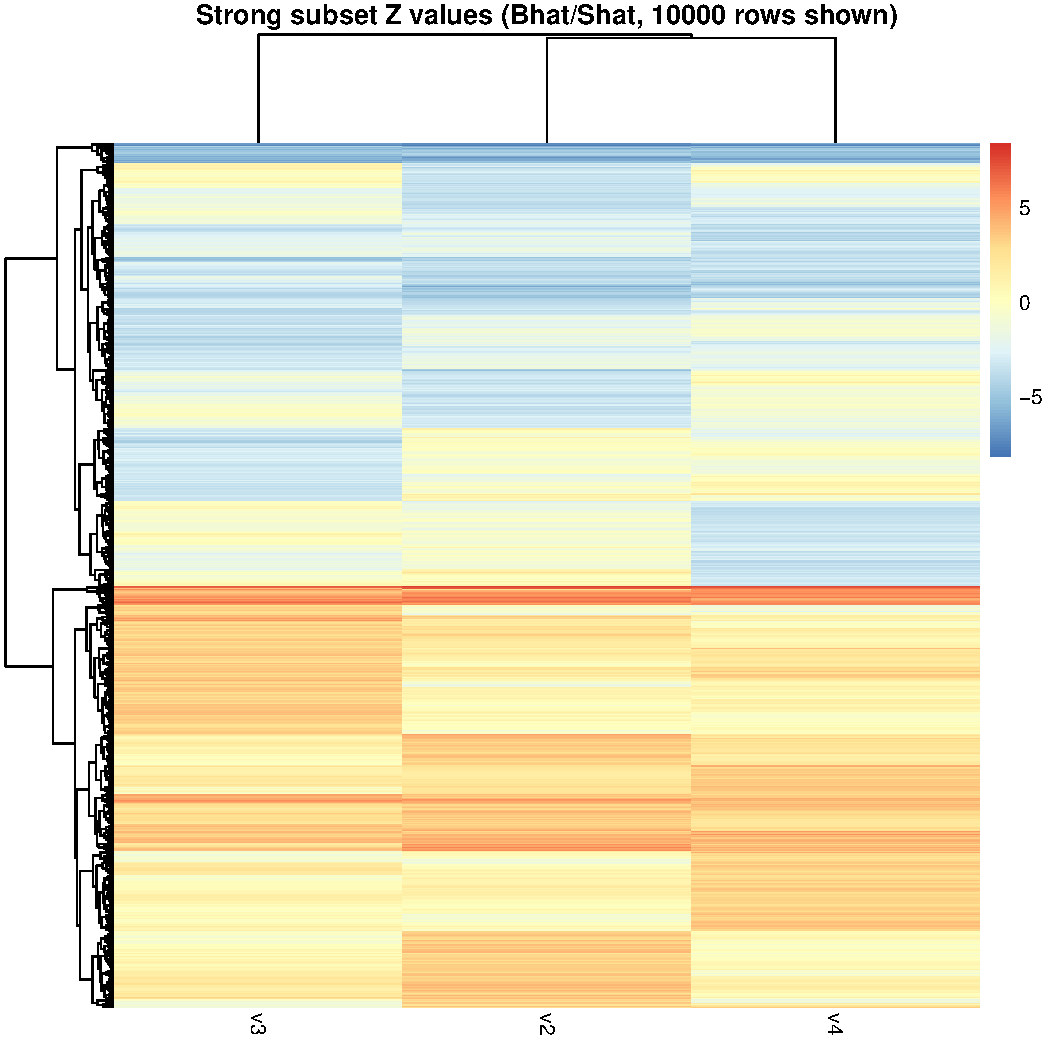
\includegraphics[width=1.0\textwidth,page=1]{mainmatter/figures/chapter_03/mash_mega/mashr.strong_subset_zval_heatmap.cisDist_1e6.sampleAcThresh_15.randomSubsetN_200000.pdf}
%     \caption{Clustering of within-timepoint Z scores in the strong mashr subset (random sample of 10000/45962 tests), confirming the presence of strong condition-specific effects.}
%     \label{fig:hird_mashr_strongSubset_Z_mega}
% \end{figure}

The \software{mashr} model was trained on a random subset of 200000 tests, using the Exchangeable Z-scores model\autocite{urbut2018FlexibleStatisticalMethods}.
The correlation of null tests between conditions, critical to account for due to the repeated measures structure of the data, was estimated using \software{mashr::estimate\_null\_correlation}.
% \todo{note this is critical, since we know a priori not independent due to eqtl sharing}
The fitted model was used as a prior to compute posterior effects and standard errors for all tests through shrinkage.
% Stephens, M. (2016). False discovery rates: A new deal. Biostatistics, kxw041. https://doi.org/10.1093/biostatistics/kxw041
% analogous to a false discovery rate, but more stringent because it requires true discoveries to be not only nonzero, but also correctly signed.
%
% Also see:
% type s error rates for classical and bayesian single and multiple comparison procedures
% Why We (Usually) Don’t Have to Worry About Multiple Comparisons (2012)
% Beyond Power Calculations: Assessing Type S (Sign) and Type M (Magnitude) Errors (2014)
A condition-specific Bayesian measure of significance \gls{lfsr} is returned, 
the probability that the declared sign of the effect is incorrect \autocite{stephens2016FalseDiscoveryRates}.
Note that \software{mashr} is the multiple-condition extension of \software{ashr}, 
previously used in \cref{subsubsec:hird_dge_multipleTestingCorrection} for computing posterior effects and their significance in \gls{DGE} analyses.

\subsubsection{Defining shared and response eQTLs}

Many of the tested variants for each gene will be in high \gls{LD}.
% qtls.merged[, signif_rank := frank(qtls.merged, lfsr, -INFO, -MAF_sample, SNP_gene_TSS_dist, POS)]
To unambiguously select a lead \gls{eQTL} variant per gene, I selected the variant with the lowest lfsr in any condition, 
breaking ties by highest imputation INFO, highest \gls{MAF}, most upstream of the \gls{TSS}, and genomic coordinate.
Sharing was then evaluated for that gene-variant pair across all three conditions.

Thresholding on the lfsr is not appropriate for determining sharing, as the difference between significant and non-significant effect estimates in two conditions is not necessarily significant\autocite{schenker2001JudgingSignificanceDifferences,gelman2006DifferenceSignificantNot}.
% Not just use lfsr thresholds:
\autocite{urbut2018FlexibleStatisticalMethods} provides a heuristic that two effects are shared by magnitude if they have the same sign, and are also within a factor of 2 of one another,
but this does not consider the posterior standard error of the estimates.
% Also see:
% https://andrewpwheeler.wordpress.com/2016/10/19/testing-the-equality-of-two-regression-coefficients/
    % Var(A-B) = Var(A) + Var(B) - 2*Cov(A,B)
    % NOTE: Assumes that Cov is 0, this is anticonservative when Cov is actually positive.
% Also: notes from 2018-10-11 on wald test, and comments on sharing_func in get sharing script
% Also: USING THE CORRECT STATISTICAL TEST FOR THE EQUALITY OF REGRESSION COEFFICIENTS https://onlinelibrary.wiley.com/doi/abs/10.1111/j.1745-9125.1998.tb01268.x
Between a pair of effects in two conditions, I compute a \textit{z}-statistic for the difference in effects \autocite{clogg1995StatisticalMethodsComparing,schenker2001JudgingSignificanceDifferences}:

\begin{equation}
z = \frac{\beta_x - \beta_y}{\sqrt{\sigma_x^2 + \sigma_y^2 - 2\sigma^2(x, y)}}
\end{equation}

This strategy has been applied to call reQTLs by \autocite{kim-hellmuth2017GeneticRegulatoryEffects},
% Actually we can get:
% PosteriorCov
% Q x Q x J array of posterior covariance matrices, if the output_posterior_cov = TRUE.
assuming posterior pairwise covariance of effects is zero $\sigma^2(x, y)$.
\todo{not sure whether this is conservative or anti-conservative}
\todo{mashr does not provide by default}
% TODO we consider the var cov matrix of coefficients here, not the expressions
% TODO this is convservative unless corr is >0.5?
% NOTE: A Wald test uses W ~ chisq(1), equivalent to sqrt(W) ~ N(0, 1).
A Wald test \pvalue{} for the difference can be computed, as under the null hypothesis of zero difference, asymptotically $z \sim \mathcal{N}(0, 1)$.
I use nominal \pvalue{} < 0.05 as a heuristic threshold (like the mashr recommended 2-fold threshold) to define reQTL effects that are strong, rather than a formal measure of significance.
% TODO: but ideally, define reQTL strength as an ordering, not by thresholding
% TODO: emph the progression from simple lfsr (e.g. gtex ccqtl, huang2020NeonatalGeneticsGene) -> mashr 2-fold (mashr) -> to want to look at se too
Effects are only compared if at least one of the two effects has lfsr < 0.05, to avoid sharing being driven by null effects.

\subsubsection{Replication of eQTLs in a reference dataset}

To validate the \gls{eQTL} mapping approach, I estimate the replication of significant eQTLs in a large independent reference.
% Define eGene here TODO
Due to the lack of large sample size \gls{eQTL} maps specific to \gls{PBMC}, I use the GTEx v8 whole blood dataset as my reference dataset (\autocite{thegtexconsortium2020GTExConsortiumAtlas}, n=670, 51.2\% eGene rate).
For lead variants called as significant in the \gls{HIRD} dataset at a given lfsr threshold, I lookup the nominal \pvalue{} for that variant in GTEx (where the variant exists in both datasets).
I applied \software{qvalue::qvalue\_truncp} to estimate the proportion of those GTEx nominal \pvalues{} that are null ($\pi_0$), the compute a measure of replication $\pi_1 = 1 - \pi_0$.

The mega-analysis has comparable replication rate to \gls{RNAseq}-only analysis for shared \glspl{eQTL} at moderately stringent \gls{lfsr} thresholds up to $10^{-5}$ (\cref{fig:hird_eQTL_pi1vsGTExWholeBlood}).
Past this, as the $\pi_1$ procedure assumes a well-behaved \pvalue distribution in $\left[0, 1\right]$, 
reliability declines due to the number of \pvalues{} being too small\footnote{\url{https://github.com/StoreyLab/qvalue/pull/6\#commitcomment-26277751}}, or the maximum \pvalue{} being too far from 1.
The numbers of \glspl{reQTL} were too low to assess replication using this method, and one might not expect them to replicate in a baseline dataset such as GTEx whole blood, especially for those \glspl{reQTL} significant only at post-vaccination timepoints.
As the mega-analysis has a higher eGene rate (\percentage{0.5075166} vs. \percentage{0.29914529915}) compared to the \gls{RNAseq}-only analysis, with similar replication,
I assume this represents a power advantage from having larger a sample size, rather than technical effects from merging the expression data.
% \todo{add comment on number of eGenes. the real reason here is prob robustness?}
% \todo{RNAseq does test about 7000 more genes though...}
% TODO: this approach may overestimate the replication rate as it does not take the direction or magnitude of eQTL effects into account.

\begin{figure}
    \centering
    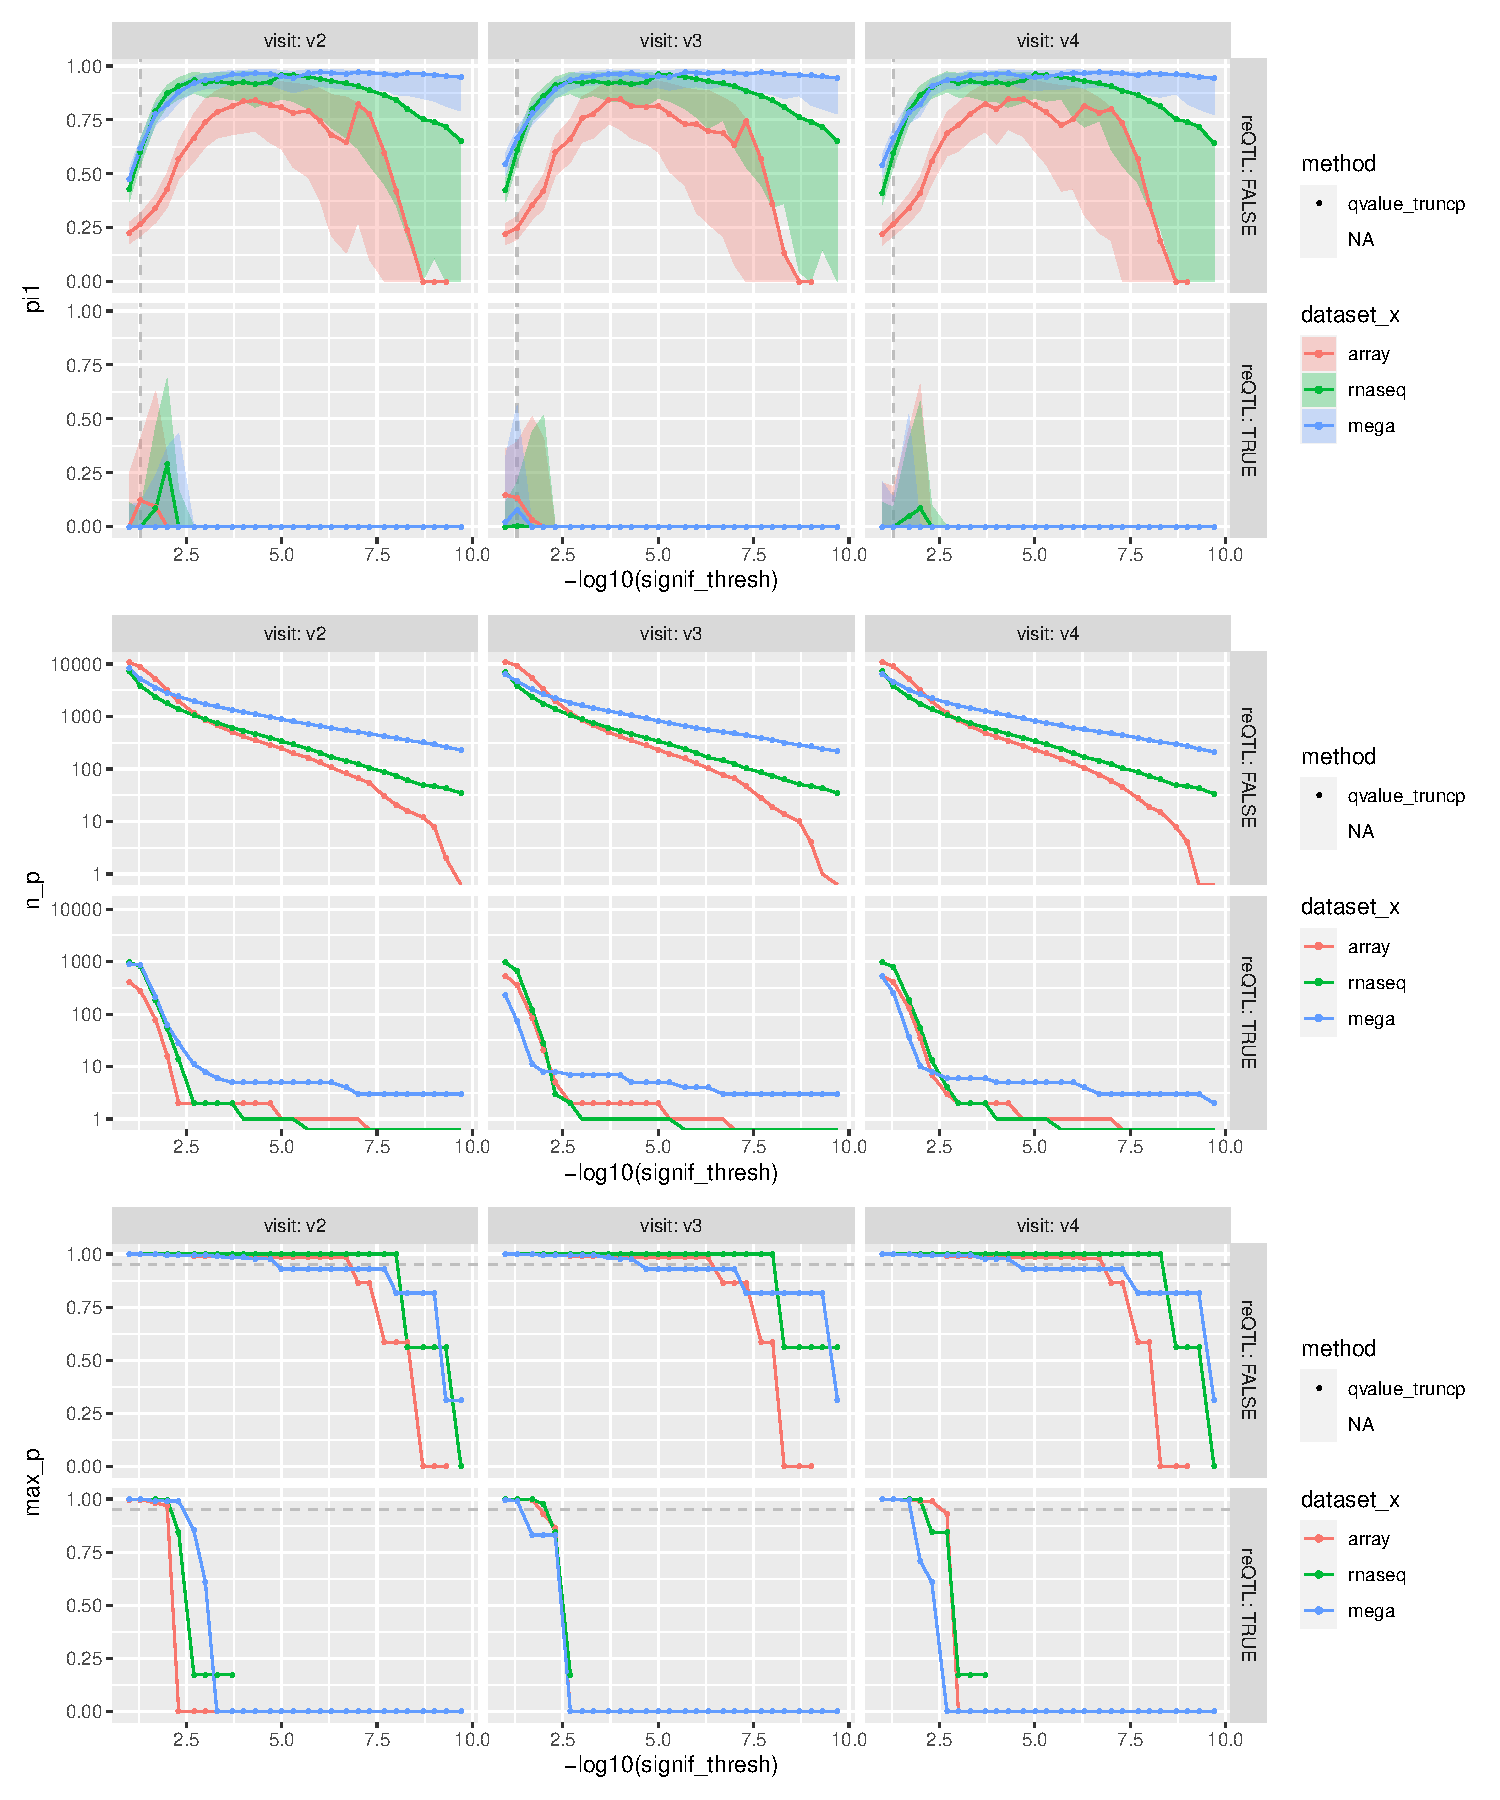
\includegraphics[width=1.0\textwidth,page=1]{mainmatter/figures/chapter_03/compute_pi1.pi1_by_thresholds.pdf}
    \caption{
        Effect of \gls{HIRD} lfsr threshold on GTEx whole blood replication rate ($\pi_1$), number of \pvalues{} used to compute $\pi_1$, and maximum \pvalue{} among those \pvalues{}; 
        for shared and \gls{reQTL} called from the array-only, \gls{RNAseq}-only and mega-analysis pipelines. 
        Shaded region for $\pi_1$ represents the 5th-95th percentile range of 1000 bootstraps.
    }
    \label{fig:hird_eQTL_pi1vsGTExWholeBlood}
\end{figure}
        % TODO: 10000?

\subsection{Genotype interactions with cell type abundance}
\label{subsec:hird_reQTL_methods_cellTypeInteraction}

% TODO: note moderator is more likely, but mediator G -> CC -> E is also possible

% TODO: see kim2020.pdf for causalgraphs for pre-post

% TODO need a DAG on why reqTL in vivo cannot guarantee causality of G on change in E

% \todo{be more specific: "moderator", 'modify'?????}
% NOTE: Effect modification can be present with no interaction; interaction can be present with no effect modification. \autocite{vanderweele2009DistinctionInteractionEffect}
% TODO: In regression, one of the assumptions is the additive assumption. This assumption states that the influence of a predictor variable on the dependent variable is independent of any other influence
% Holding all else equal Implies beta does not depend on other predictors
% https://journals.lww.com/epidem/Fulltext/2009/11000/On_the_Distinction_Between_Interaction_and_Effect.16.aspx
% https://significantlystatistical.wordpress.com/2014/12/12/confounders-mediators-moderators-and-covariates/
% TODO: why?
% happens if there is cell type-specific relevance of g
% cause cell type affects g->e i.e. symetrically, geno affects c -> e
% Figure out what DAG model causes a reQTL in bulk to not represent causality of G -> change in e
If the abundance of a particular cell type does truly modify the \gls{eQTL} effect, 
then an interaction term between genotype and cell type abundance is required.
A \textit{ceteris paribus} interpretation no longer makes sense,
as the effect of genotype holding cell type abundance constant depends on what value of cell type abundance you choose.
% \todo{point is, doesn't make sense to assume the genotype effect is the same at all levels of cell type abundance}
% TODO: what is the effect of genotype going up a unit holding cell props constant? well, actually it depends on the constant....
% i.e. this is non-addititivty 
otherwise the regression slope of the \gls{eQTL} term will be biased;
% TODO: OVB by setting interaction coefficient to zero
% http://consirt.osu.edu/wp-content/uploads/2014/10/CONSIRT-Working-Papers-Series-9-Mikucka_Sarracino_Dubrow.pdf
% Most importantly, the figures document thatwrongly  omitting  an  interaction  term  (Figure  3)  can  bias  the  estimates  much  more  thanwrongly including an interaction term (Figure 4).
one cannot adjust for this modification just by including the main effect for cell type abundance.
% \todo{misspecification}
% TODO: if the data gen process is so, the simply a misspecification to not have it
% referred to in econometrics as "functional form misspecification", a special case of OVB.
% e.g. https://www.econometrics-with-r.org/9-2-ttivomra.html
% basically, if you need a diff slope over levels of modifying var, it can't possibly have one without it being in the model
% if you need var slopes, but only allow var intercepts
%
% One  specific case,  functional  form  misspecification,  occurs  when  the  omitted  variable  is  a function of another explanatory variable in the model (Wooldridge, 2002).
%
% https://stats.stackexchange.com/questions/263324/how-can-the-regression-error-term-ever-be-correlated-with-the-explanatory-variab
% the realisation of the error term, the residuals, is forced to be uncorrelated, hence you get a biased estimate
Given the modest sample size, I use the two-step approach used by others\autocite{westra2015CellSpecificEQTL,peters2016InsightGenotypePhenotypeAssociations,kim-hellmuth2017GeneticRegulatoryEffects,davenport2018DiscoveringVivoCytokineeQTL},
where tests for interaction are only performed at a subset of tests, often the lead \gls{eQTL} variant for each gene.
% Unfortunately, there seems to be no consensus between these studies for controlling the interaction effect tests for multiple testing.
%
% Strange custom 5% FDR: westra2015CellSpecificEQTL
% Bonferroni: kim-hellmuth2017GeneticRegulatoryEffects
% Benjamini-Hochberg FDR: kim-hellmuth2017GeneticRegulatoryEffects
% Benjamini-Hochberg procedure, and a 0.15 FDR threshold: peters2016InsightGenotypePhenotypeAssociations
%
% https://www.jmp.com/support/help/en/15.2/index.shtml#page/jmp/effect-heredity.shtml
% The principle of effect heredity relates to the inclusion in the model of lower-order components of higher-order effects. The motivation for this principle is observational evidence that factors with small main effects tend not to have significant interaction effects.
% NOTE: this is not strictly effect heredity, as I do not consider the significance of cell proportion terms
%
% TODO: dodgy, review this paper again
The key to the two-stage approach is that if the estimates for the interaction effect are sufficiently independent from the estimates of the main effect from main-effect only models,
the type I error can be controlled based on the number of interactions that are actually tested, rather the number of interactions that could have been tested for\autocite{kooperberg2008IncreasingPowerIdentifying,peters2016InsightGenotypePhenotypeAssociations}.
It is unclear whether this assumption holds, as the size of the main effect may contribute to power for detecting interaction effects.
As the main purpose of the interaction analyses is scanning for cell type effects at detected \glspl{reQTL},
I chose to test for interactions only at the lead \gls{eQTL} variant for each gene with a significant main \gls{eQTL},
then apply the \gls{BH} \gls{FDR}, as used by others\autocite{peters2016InsightGenotypePhenotypeAssociations,kim-hellmuth2017GeneticRegulatoryEffects}.

Models in interactions between genotype and other predictors were fit using \software{lme4qtl}.
The model specification identical to \cref{eq:hird_reQTL_limix_model}, with the addition of three interaction terms between genotype and each xCell score.
Significance is assessed using the likelihood-ratio test versus the nested model with no interaction terms.
% \todo{can we interpret with peer in? add note of CLAIM here that although peer is correlated with xcell, interactions are only formed with xcell, so the interaction term can be interpreted per unit of genotype increase when xcell=0}

% TODO:
% o	reQTLs had no enrichment in particular.
% but in the set of genes with Cell type interactions -> do a tmod (enriched?)


\subsection{Gene set enrichment analyses}

Ranked gene set enrichment analyses with \software{tmod::tmodCERNOtest} were conducted as described in \cref{subsec:hird_dge_geneSetEnrichment},
using \glspl{BTM} from \textcite{li2013MolecularSignaturesAntibody} (prefixed \enquote{LI}).

Gene set overrepresentation analyses were run with \software{gprofiler2::gost} \autocite{raudvere2019ProfilerWebServer},
which derives gene sets from
    Gene Ontology,
    pathway databases (KEGG, Reactome, WikiPathways),
    regulatory motif databases (TRANSFAC, miRTarBase),
    pathway databases (KEGG, Reactome, WikiPathways),
    protein databases (Human Protein Atlas, CORUM),
    and phenotype ontologies (HP).
The 13570 genes assayed by both array and \gls{RNAseq} were used as a custom background set (\texttt{domain\_scope='custom'}).
The default g:SCS method was used to control for multiple testing while accounting for the hierarchical structure of certain gene set databases like the Gene Ontology.

\subsection{Statistical colocalisation}
\label{subsec:hird_reQTL_coloc}
\todo{new subsection}

Published \gls{GWAS} and \gls{QTL} summary statistics were downloaded for statistical colocalisation with per-timepoint \gls{HIRD} \gls{eQTL} summary statistics.
Clinical blood count \gls{QTL} maps generated by \textcite{astle2016AllelicLandscapeHuman} in \num{173480} European-ancestry participants were downloaded from \url{ftp://ftp.sanger.ac.uk/pub/project/humgen/summary_statistics/human/2017-12-12/hematological_traits/}.
\gls{eQTL} maps in 15 \gls{FACS}-sorted immune cell types generated by \textcite{schmiedel2018ImpactGeneticPolymorphisms} in a multi-ethnic cohort of 91 donors,
were downloaded from the eQTL Catalogue (\autocite{kerimov2020EQTLCatalogueCompendium}, release 1 - January 2020, \url{https://www.ebi.ac.uk/eqtl/}).
These included
three naive innate immune cell types: 
    classical monocytes (CD14\textsuperscript{high}CD16\textsuperscript{-}),
    non-classical monocytes (CD14\textsuperscript{-}CD16\textsuperscript{+}),
    and \gls{NK} cells;
four naive adaptive immune cell types:
    B cells, CD4+ T cells, CD8+ T cells, and regulatory T cells (Treg);
CD4+ T cells and CD8+ T cells stimulated with anti-CD3 anti-CD28 for 4 hours;
and six CD4+ memory T cell subsets:
    Th1, Th1/Th17, Th17, Th2, and memory Tregs.
\gls{IBD} \gls{GWAS} summary statistics generated by \textcite{delange2017GenomewideAssociationStudy} in a total of \num{59957} European ancestry samples were downloaded from \url{https://www.ebi.ac.uk/gwas/studies/GCST004131}.
Datasets were converted to GRCh38 coordinates with \software{rtracklayer::liftOver},
and harmonised to a standard format, matching variants between studies by genomic position and effect allele.

Multi-trait Bayesian colocalisation was performed using \software{HyPrColoc} \autocite{foley2019FastEfficientColocalization}.
\software{HyPrColoc} uses the pattern of per-variant summary statistics (betas and standard errors) from multiple traits in a locus to partition traits into clusters, where each cluster contains traits that share a causal variant.
This can be seen as a multi-trait extension of pairwise Bayesian colocalisation methods such as \software{coloc} \autocite{giambartolomei2014BayesianTestColocalisation}.
Multi-trait colocalisation is more powerful than pairwise colocalisations for detecting causal variants shared between more than two traits,
and large numbers of traits can be analysed simultaneously in a computationally efficient manner.
The method formally assumes that studies generating the summary statistics for each trait are independent,
but performs well even when there is complete sample overlap between traits \autocite{foley2019FastEfficientColocalization}.
% https://github.com/jrs95/hyprcoloc/issues/1
% As the model assumes there is at most one causal variant per phenotype, the way the model is set up there is no need to consider LD between variants. This follows from the Giambartolomei coloc method (PMID: 24830394), on which HyPrColoc is based.
% The LD matrix is only required in HyPrColoc to modify the variant priors when the traits are from non-overlapping samples in conjunction with a phenotype correlation matrix (there is a complex argument as to why this is necessary, which @cnfoley can give you). Although, in simulations treating phenotypes as if they were from independent samples, even if they were not, often out-performed trying to account for the possible correlation between phenotypes caused by analysing the phenotypes in the same participants. So, our general advice is to just run the standard model, and to not worry about global phenotype correlation caused through analysis of overlapping samples.
If studies are non-independent, 
it is assumed the \gls{LD} structure is the same across those studies (which holds in the case of multiple \gls{QTL} maps generated from the same individuals).
Each trait is assumed to have no more than one causal variant in the locus.
Finally, it is assumed the causal variants for each trait are present in the input.

As with any Bayesian colocalisation method, the choice of priors and other algorithm parameters is influential.
\software{HyPrColoc} implements variant-level priors where the prior depends on the number of traits a variant is causally associated with.
\texttt{prior.1} is the prior probability that a variant is causal for one trait (default = \num{1e-4}) and
1 - \texttt{prior.2} specifies the prior probability that a variant is causal for an additional trait, given it is causal for one trait (default = \num{0.98}).
The prior for a variant being causal for a third trait given it is causal for two traits is $1-(\texttt{prior.2})^2$, and so on.
In the two trait case, the setup is identical to \texttt{coloc} \autocite{giambartolomei2014BayesianTestColocalisation}.
\texttt{prior.2} tends to be more influential than \texttt{prior.1}, as it controls the probability of association with more and more traits.

The posterior probability of colocalisation for a cluster of traits is the product of regional association and alignment probabilities.
% Calculated from variant level probabilities?
The regional association probability is the probability there is a shared association region within the locus for all the traits in the cluster, containing one or more causal variants.
The alignment probability is the probability that regional association is due to a single causal variant, rather than one or more variants in strong \gls{LD}. 
A branch and bound algorithm is run, starting with all traits in one cluster,
then recursively partitioning traits into subsets, assessing regional association and alignment probabilities for subsets at each iteration.
The end result is clusters of traits sharing a causal variant, with each cluster having a distinct causal variant.
% Traits left in their own cluster do not colocalise with any other traits.
Only clusters with more than one trait and regional association and alignment probabilities above \textit{reg.thresh} (default=0.5) and \texttt{align.thresh} (default=0.5) are reported.

% NOTE: https://rdrr.io/github/jrs95/hyprcoloc/f/vignettes/hyprcoloc.Rmd
In sensitivity analyses using the \software{sensitivity.plot} function,
% As the number of traits in the sample increases the default choice of $prior.1$ may be become increasingly inappropriate.
% However, to guide analyses we suggest comparing results using the default $10^{-4}$ with those when $prior.1 = 10^{-5}$, i.e. an order of magnitude reduction in "prior.2", for sensitivity analyses.
I fixed the less influential \texttt{prior.1} at the default of \num{1e-4}, 
then iterated over combinations of
% When using the variant specific prior, results tend to be most sensitive to the choice of $prior.2$ as this controls the prior probability of each additional colocalized trait.
four choices of \texttt{prior.2} (0.98, 0.99, 0.995, 0.999),
% Note, these parameter choices are a consequence of extensive testing in simulation scenarios, aiming to maximise the true detection rate whilst minimising the number of false positives. We therefore DO NOT recommend reducing the value of either of these parameters. The defaults should be viewed as lower bounds.
% We therefore DO NOT recommend reducing the value of either of these parameters. The defaults should be viewed as lower bounds.
five choices of \texttt{reg.thresh} (0.5, 0.6, 0.7, 0.8, 0.9),
and five choices of \texttt{align.thresh} (0.5, 0.6, 0.7, 0.8, 0.9).
Each range starts at the default value and becomes more stringent, 
requiring stronger and stronger evidence for clusters of colocalised traits to be identified.

\section{Results}
\todo{heavy rewrites all throughout}

\subsection{Mapping reQTLs in the HIRD cohort}

To characterise the effect of common host genetic variation on expression response to Pandemrix,
I mapped cis-\glspl{eQTL} for each gene (\SI{\pm1}{\mega\bp} of the \gls{TSS}) within each timepoint condition (baseline, day 1, and day 7),
then conducted joint analysis of all three timepoints with \software{mashr} \autocite{urbut2018FlexibleStatisticalMethods} to obtain per-timepoint posterior effect sizes, posterior standard errors, and measures of significance (\gls{lfsr}).
% \todo{quick note on mega-analysis and GTEx replication here}
At \gls{lfsr} < 0.05, \num{6887/13570} genes (\percentage{0.5075166}) were eGenes (genes with a significant \gls{eQTL}) in at least one timepoint.
The most significant tested variant over all timepoints was selected as the lead variant for each gene,
then \glspl{reQTL} were defined by comparing the effect size of this lead variant between each pair of timepoints.
This guards against differences in effect size from differential tagging efficiency (of an assumed single causal variant), which might occur if different variants were compared across timepoints.
\cref{fig:hird_eQTL_upset_mega} shows patterns of sharing over timepoints for the lead variant for each of the \num{13570} genes,
illustrating the difference between calling \gls{reQTL} using a significance threshold versus the difference in betas approach.
For example, there were 85 \gls{eQTL}-eGene pairs significant only at day 1 post-vaccination ($lfsr < 0.05$); of these only \num{40/85} are \glspl{reQTL} by the difference in betas method.
The difference in betas method is more strict because calling by significance alone would call a \gls{reQTL} for an \gls{eQTL} with lfsr = 0.049 at baseline and lfsr = 0.051 at day 1, even if the effect sizes are similar.

The largest number of eGenes was detected at baseline, reflecting the larger sample size compared to other timepoints.
Most \glspl{eQTL} were shared across timepoints; 
these were also the strongest \glspl{eQTL} in terms of both maximum absolute beta and \gls{PVE} across timepoints, highlighting the power advantage for mapping shared effects granted by joint analysis.
\num{1154/6887} (\percentage{0.1675621}) \glspl{eQTL} were classified as \glspl{reQTL} based on difference in effect size (beta) between any pair of timepoints (nominal p < 0.05).
Of these, 
\num{690/1154} were \glspl{reQTL} in both baseline- day 1 vs. baseline and day 7 vs. baseline, 
and only \num{23/1154} were unique to the day 7 vs. day 1 comparison, 
indicating most \gls{reQTL} effects were differences between pre- and post- vaccination (\cref{fig:hird_reQTL_pairwise_venn}).

\begin{figure}
    \centering
    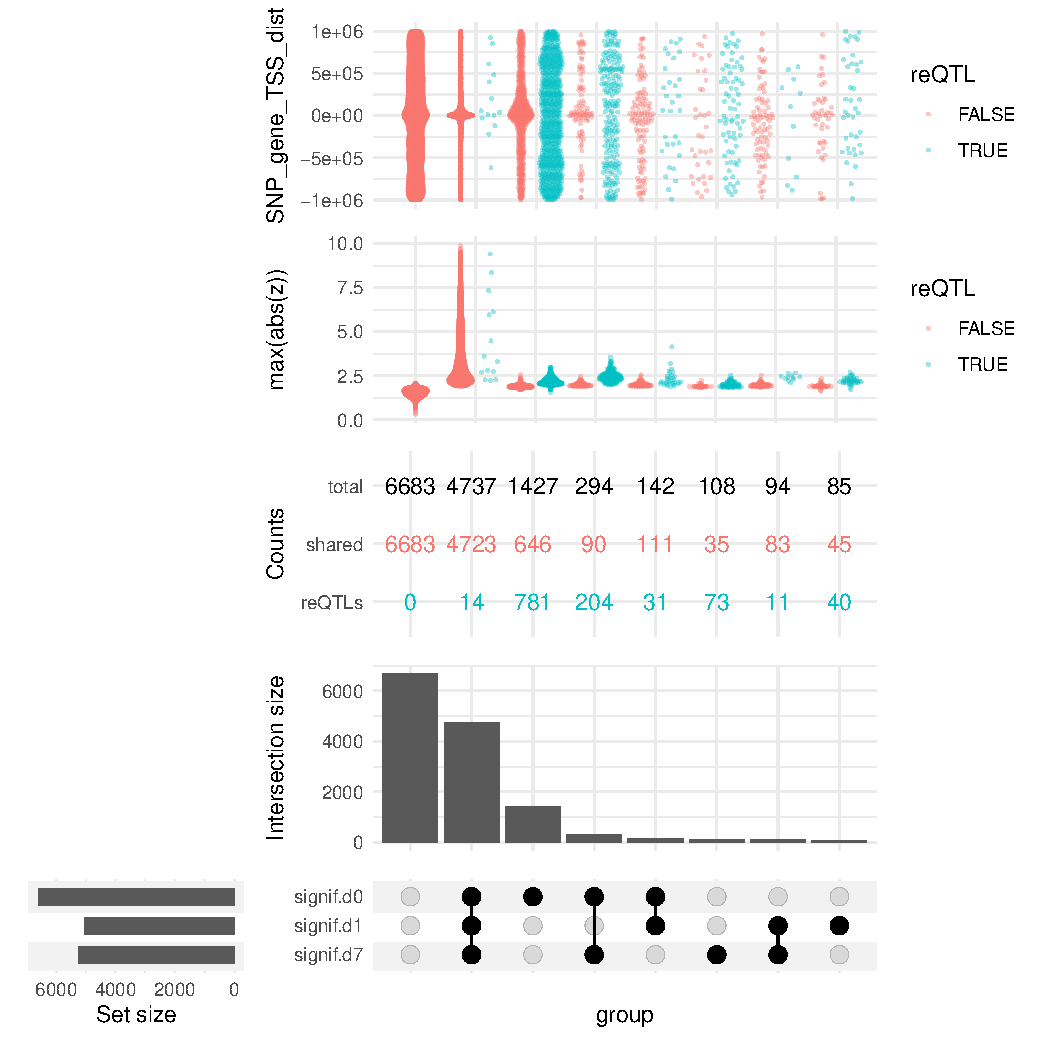
\includegraphics[width=1.0\textwidth]{mainmatter/figures/chapter_03/compare_dge_eqtl.upset.pdf}
    \caption{
        \textbf{Summary of HIRD eQTL mapping at 13570 genes in a mega-analysis of array and RNAseq, binned by patterns lead variant significance over the three timepoints.}
        The most significant variant for each gene over all timepoints was chosen as the lead variant.
        Significant eQTLs (lfsr < 0.05) were found at \num{6887/13570} eGenes.
        These were classified as reQTLs if there was a significant difference in beta (nominal p < 0.05) between any pair of timepoints,
        given that the eQTL was significant in at least one of those two timepoints.
        Counts of shared and reQTLs; and distribution of maximum beta and \gls{PVE} across timepoints, for variants in each bin are shown.
    }
    \label{fig:hird_eQTL_upset_mega}
\end{figure}

\begin{figure}
    \centering
    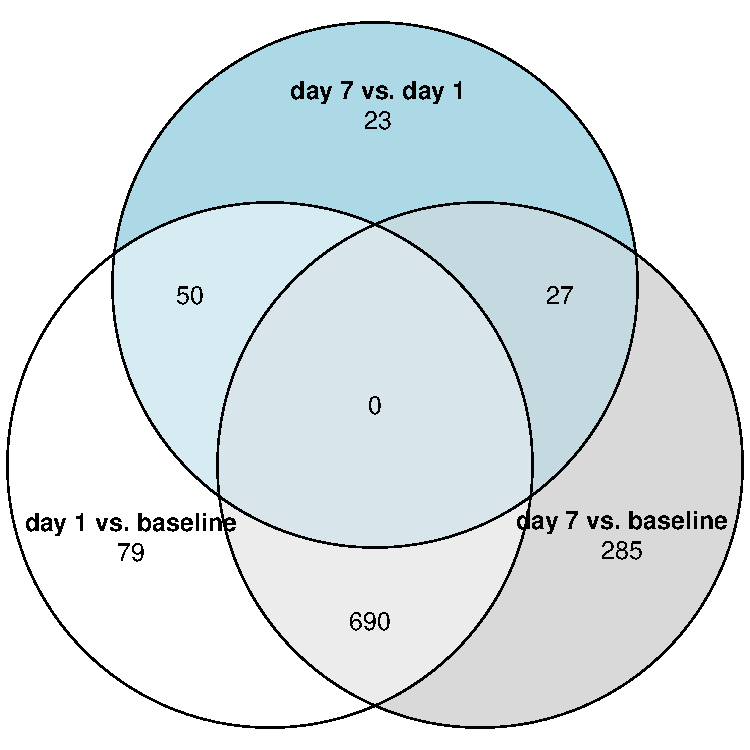
\includegraphics[width=0.6\textwidth]{mainmatter/figures/chapter_03/compare_dge_eqtl.pairwise_reQTL_venn.pdf}
    \caption{
        \textbf{\glspl{reQTL} were observed for 1154 unique eGenes, where the lead \glspl{eQTL} had a significant difference in beta between pairs of timepoints (nominal p < 0.05).}
    }
    \label{fig:hird_reQTL_pairwise_venn}
\end{figure}

\subsection{Characterising reQTLs post-vaccination}

To characterise the eGenes associated with post-vaccination \glspl{reQTL},
I ranked eGenes by the increase in \gls{PVE} for their associated \glspl{reQTL} from baseline to day 1 and baseline to day 7,
then performed ranked gene set enrichments with \software{tmod::tmodCERNOtest}.
%
% Possible Ranking metrics for ranked enrichments
%     PVE: prefers large maf and high betas since it squares the beta. even if the beta does not change so much. ignores sign.
%     beta:
%     p: ignores sign
%     Z score:
%
The same four modules were significant at both post-vaccination timepoints:
\enquote{immune activation - generic cluster} (LI.M37.0, day 1 $\text{\gls{FDR}} = \num{1.283444e-06}$, day 7 $\text{\gls{FDR}} = \num{3.391644e-06}$),
\enquote{enriched in monocytes (II)} (LI.M11.0, day 1 $\text{\gls{FDR}} = \num{4.688999e-03}$, day 7 $\text{\gls{FDR}} = \num{1.881201e-02}$),
\enquote{cytoskeleton/actin (SRF transcription targets)} (LI.M145.0, day 1 $\text{\gls{FDR}} = \num{2.071726e-02}$, day 7 $\text{\gls{FDR}} = \num{2.036488e-02}$),
and \enquote{MHC-TLR7-TLR8 cluster} (LI.M146, day 1 $\text{\gls{FDR}} = \num{2.071726e-02}$, day 7 $\text{\gls{FDR}} = \num{2.036488e-02}$).
The enrichments are weak but consistent with immune activation driving post-vaccination \glspl{reQTL}.
Given that TLR7 and TLR8 are primarily expressed in monocytes, macrophages and \glspl{DC} \autocite{cervantes2012TLR8ForgottenRelative},
and \gene{SRF} is a regulator of the cytoskeleton in macrophages \autocite{sullivan2011SerumResponseFactor}, 
there is suggestive evidence \glspl{reQTL} may be enriched in genes specific to these phagocytotic \glspl{APC}.
\todo{this whole section has been restructured to hopefully gives a better picture of why I end up with focus on ADCY3: gene set enrichments were largely uninformative, small+opposite effects everywhere at d7, ADCY3 only strong signal at d1}
\todo{instead of only talking about the top hits, I step through a series of possible mechanisms}

Changes in \gls{PVE} do not capture changes in allelic direction.
I classified post-vaccination \glspl{reQTL} into one of three effect types:
magnified, where the beta increases after vaccination but remains the same sign;
dampened, where the beta decreases after vaccination but remains the same sign;
and opposite, where the allelic direction changes after vaccination.
As \gls{lfsr} quantifies uncertainty in the sign of the effect, I do not make this classification for \glspl{reQTL} that are not significant both at baseline and post-vaccination---the effect type for these are unclear.
The classifications are shown in \cref{fig:hird_eQTL_zSharing_vs_TSSdist_mega}, plotting all 6887 shared or \gls{reQTL} by their distance relative to the eGene \gls{TSS}.
% TODO: is the gap still there if you use beta not pm?
Shared \glspl{eQTL} have \textit{z}-statistics for difference in betas close to z, and are concentrated close to the \gls{TSS} as expected, 
\gls{reQTL} had a distribution of mostly negative \textit{z}-statistics clearly separated from the shared \glspl{eQTL} at both day 1 and 7,
and these were mostly unclear or opposite rather than dampened effect types.
Many of these unclear effects may actually be dampening, 
but as the sample size is greatest at baseline, 
dampening effects are hard to distinguish from drops in power at post-vaccination timepoints, 
whereas an opposite effect significant in both timepoints is unambiguous.
% TODO: check how many opposite effects only signifcant after shrinkage

\begin{figure}
    \centering
    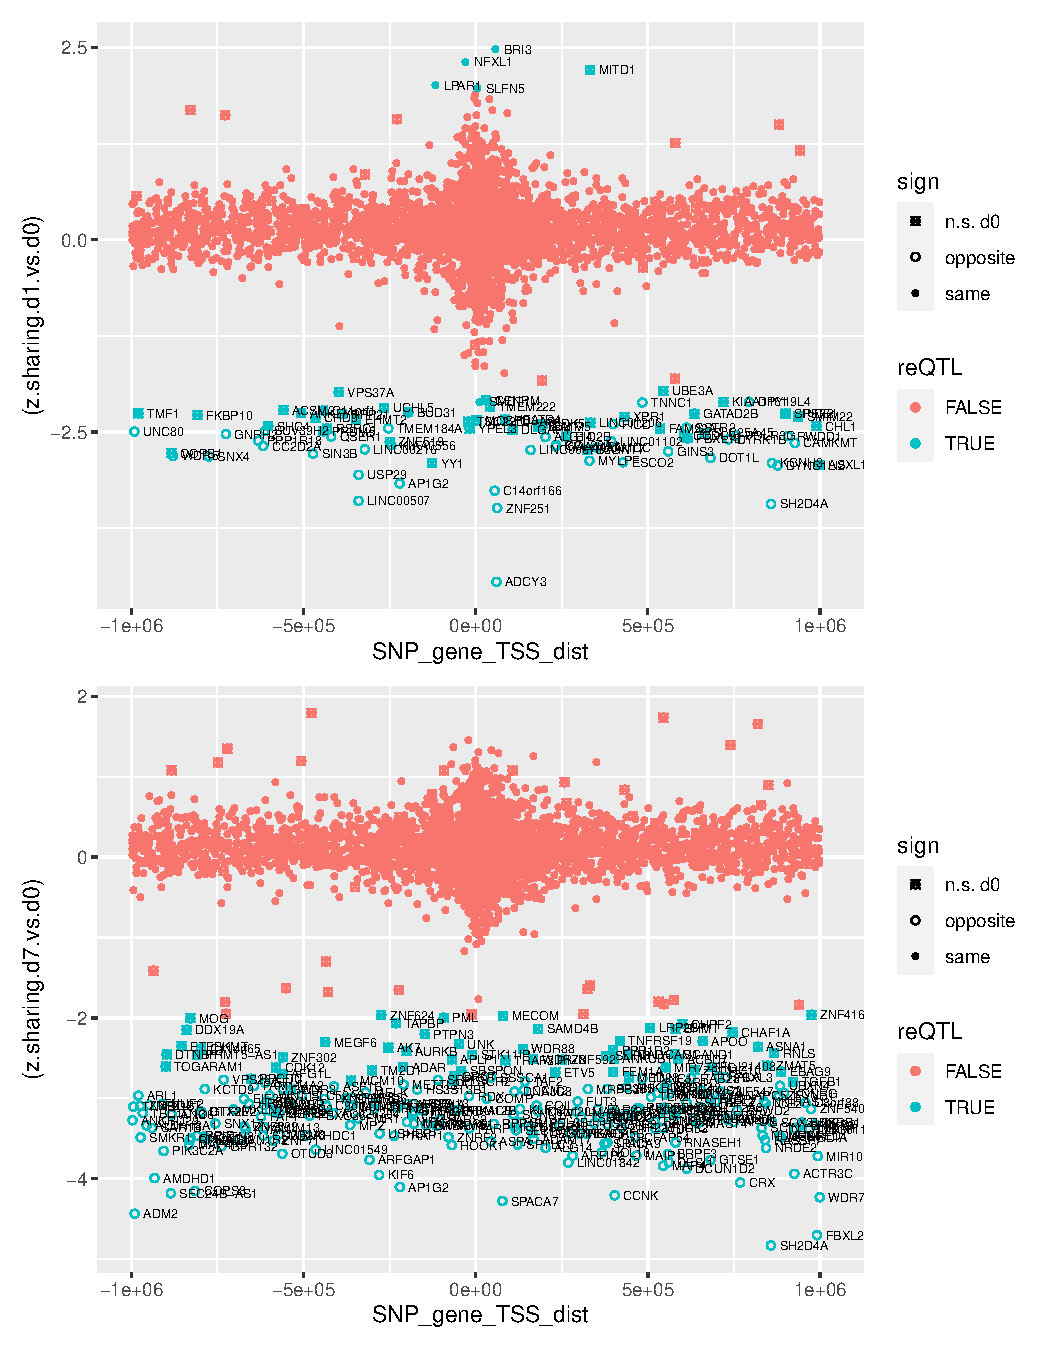
\includegraphics[width=1.0\textwidth]{mainmatter/figures/chapter_03/compare_dge_eqtl.z_sharing.vs.SNP_gene_TSS_dist.pdf}
    \caption{
        \textbf{\textit{z}-statistic for difference in beta post-vaccination versus baseline for shared and \glspl{reQTL}, stratified by distance from the eGene \gls{TSS}.}
        For each plot, all \glspl{eQTL} significant in either timepoint are shown.
        Shared \glspl{eQTL} can only have shared effect type.
        an unclear effect type indicates the \gls{eQTL} in question was not significant in both timepoints.
        Allelic direction of effect is aligned so that the beta at baseline is positive. 
    }
    \label{fig:hird_eQTL_zSharing_vs_TSSdist_mega}
\end{figure}

\glspl{reQTL} also tended to be distributed evenly across the entire \textit{cis}- window,
raising the question or whether they are enriched in false positives.
A nominal p < 0.05 threshold may be too lax for calling \glspl{reQTL},
so I applied a stronger \gls{BH} \gls{FDR} threshold of 0.2.
At this threshold, the only remaining \gls{reQTL} was at day 1 was for \gene{ADCY3} (nominal p = \num{8.676917e-06}, FDR = \num{0.1177458})---the next smallest FDR value was 0.6490604.
At day 7, 676 significant \gls{reQTL} had \gls{FDR} < 0.2, of which 221 were opposite effects.
Gene set over-representation analysis on the set of 221 eGenes to identify a shared biological signature was relatively uninformative, and revealed only one enrichment for genes \gene{PRKACB}, \gene{PRKACA}, \gene{SAR1B} and \gene{APOE} in \enquote{Plasma lipoprotein assembly} (Reactome pathway identifer R-HSA-8963898, set size = 11, adj. p = \num{0.00691834}).

\subsection{Exploring possible mechanisms generating reQTLs}

\subsubsection{Differential gene expression of reQTL eGenes}

As gene set analyses based on the effect sizes of \glspl{reQTL} at different timepoints had been largely uninformative,
I considered whether \gls{reQTL} could be characterised by shared mechanisms.
One mechanism that could generate \glspl{reQTL} effects is differential expression, where an \gls{eQTL} is not detected at baseline because the eGene is not expressed, and vaccine-stimulated upregulation reveals the effect post-vaccination.
\cref{fig:hird_eQTL_zSharing_vs_TSSdist_mega} also shows whether each eGene was up or downregulated at the timepoint based on the \gls{DGE} analyses in \cref{ch:hird_DGE}.
Visually, a large number of \gls{reQTL} occur without corresponding differential expression.
Statistically, compared to genes without reQTL,
genes with \glspl{reQTL} were less likely be differentially expressed post-vaccination at day 1 (\percentage{0.2649573} for genes with reQTL, \percentage{0.4227119} for genes without reQTL, Fisher's test p < \num{2.2e-16}).
This was also the case when restricting the scope to only eGenes (\percentage{0.2649573} for genes with reQTL, \percentage{0.4791946} for genes with shared eQTL, Fisher's test p < \num{2.2e-16}).

At day 7, 
no significant difference was observed comparing to genes without a reQTL (\percentage{0.02195609} for genes with reQTL, \percentage{0.01368555} for genes without reQTL, Fisher's test p = \num{0.05088}),
but compared to genes with shared \gls{eQTL},
genes with \gls{reQTL} were more likely to be upregulated
(\percentage{0.02195609} for genes with reQTL, \percentage{0.01068966} for genes with shared eQTLs, Fisher's test p < \num{0.005015}).
Twenty-two genes with both day 7 \gls{reQTL} and upregulated expression were strongly enriched within gene sets related to the cell cycle
(e.g. \enquote{mitotic cell cycle}, Gene Ontology biological process term GO:0000278, term size = 914, intersection size = 12, \software{gprofiler2::gost} adj. p = \num{0.0001419083}).
% Small and oppopste between cell types, can we find enrichment?
\todo{do a quick tmodHD test}
However, these 22 genes previously appeared in \cref{fig:hird_eQTL_zSharing_vs_TSSdist_mega},
all having \gls{reQTL} with decreased or opposite effect at day 7 versus baseline,
making it implausible the generating mechanism is increased detection power due to upregulation.
The enrichment for cell cycle is likely driven by the \gls{DGE} signal alone,
especially as cell cycle gene modules were detected to be strongly upregulated at day 7 in \cref{subsec:hird_dge_adaptive_immune_day7}.

The presence of \gls{reQTL} without \gls{DGE} is exemplified at the strongest
\gls{reQTL} at each day.
The only significant \gls{reQTL} on day 1 at FDR < 0.2 was for \gene{ADCY3} (\cref{fig:hird_eQTL_ploteQTL_ADCY3}).
At day 1, the \gls{PVE} for this \gls{reQTL} associated with \gene{ADCY3} explained \percentage{0.01862996} of expression variation at day 0, increasing to \percentage{0.14075782} at day 1,
yet the gene was not differentially expressed from baseline to day 1 (log2FC=\num{0.10373360}, lfsr=\num{0.2569459}).
% Overall, only 5/68 (\percentage{0.1323529}) genes with \glspl{reQTL} that explain more variation at day 1 were upregulated at day 1 vs. day 0; 5/226 (\percentage{0.02212389}) for day 7 vs. day 0.
%
% The strongest reQTL at day 7 is one such opposite sign effect;
% \gene{SH2D4A} has constitutive expression in T cells, B cells, macrophages, and \glspl{DC},
% encoding a adapter protein involved in intracellular signal transduction\footnote{\url{https://doi.org/10.1111/j.1600-065X.2009.00829.x}}.
At day 7 the strongest \gls{reQTL} was at \gene{SH2D4A} (nominal p difference in betas = \num{1.369564e-06}, BH FDR = \num{0.01747935}, \cref{fig:hird_eQTL_ploteQTL_SH2D4A}).
Here, the \gls{reQTL} variant explained similar amounts of expression variation at day 0 (\gls{PVE}=\percentage{0.08229266}) and day 7 (\gls{PVE}=\percentage{0.08956865}), with opposite directions of effect (\cref{fig:hird_eQTL_ploteQTL_SH2D4A}).
Again, there was no differential expression.
There is strong evidence that many post-vaccination \glspl{reQTL} are generated by mechanisms unrelated to \gls{DGE}.

\begin{figure}
    \centering
    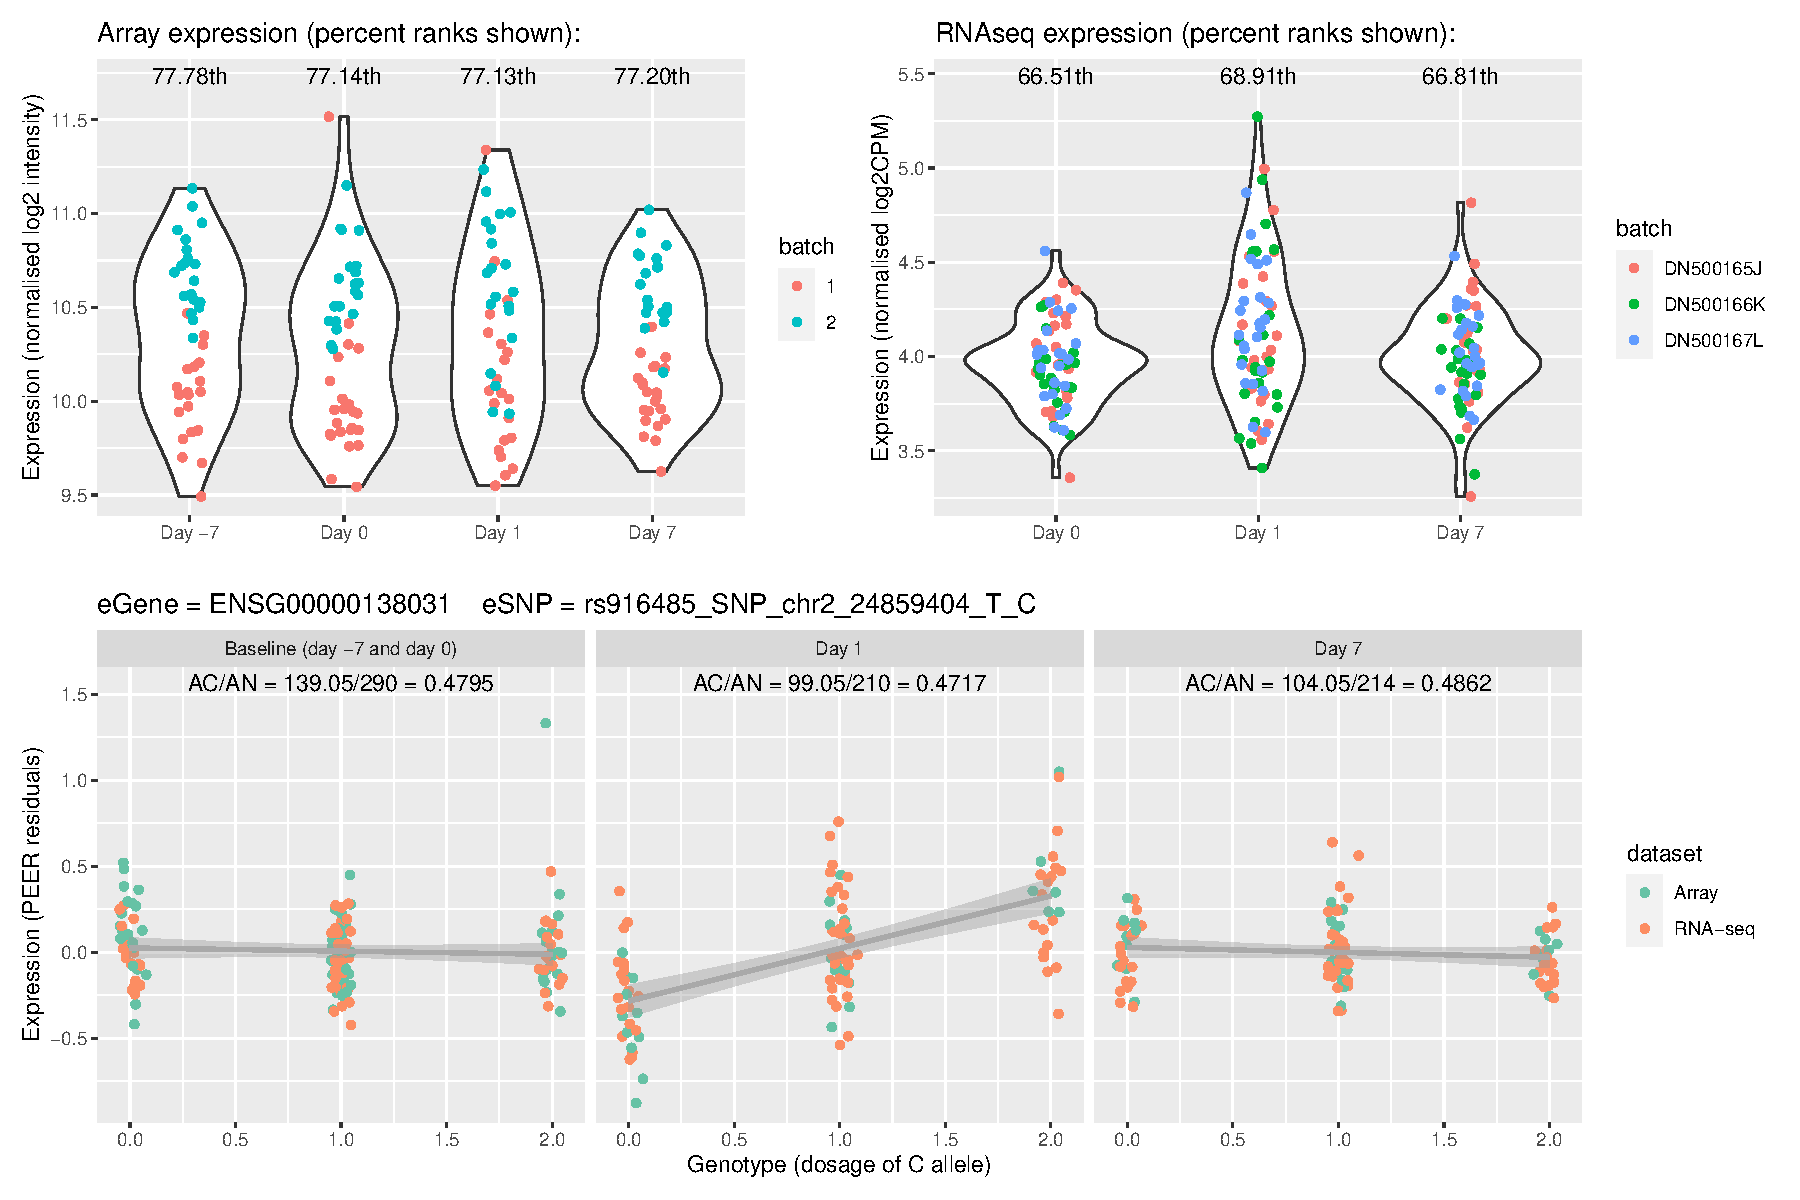
\includegraphics[width=1.0\textwidth,page=1]{mainmatter/figures/chapter_03/plot_dge_eqtl_genotypes.ENSG00000138031,rs916485_SNP_chr2_24859404_T_C.pdf}
    \caption{
        \textbf{Expression and lead \gls{eQTL} of \gene{ADCY3} over study timepoints.}
        Normalised array (top-left) and \gls{RNAseq} (top-right) expression before batch effect correction with ComBat and \gls{eQTL} mapping. 
        Bottom: \gls{eQTL} effects at each timepoint condition in the mega-analysis of array and \gls{RNAseq} data.
    }
    \label{fig:hird_eQTL_ploteQTL_ADCY3}
\end{figure}

\begin{figure}
    \centering
    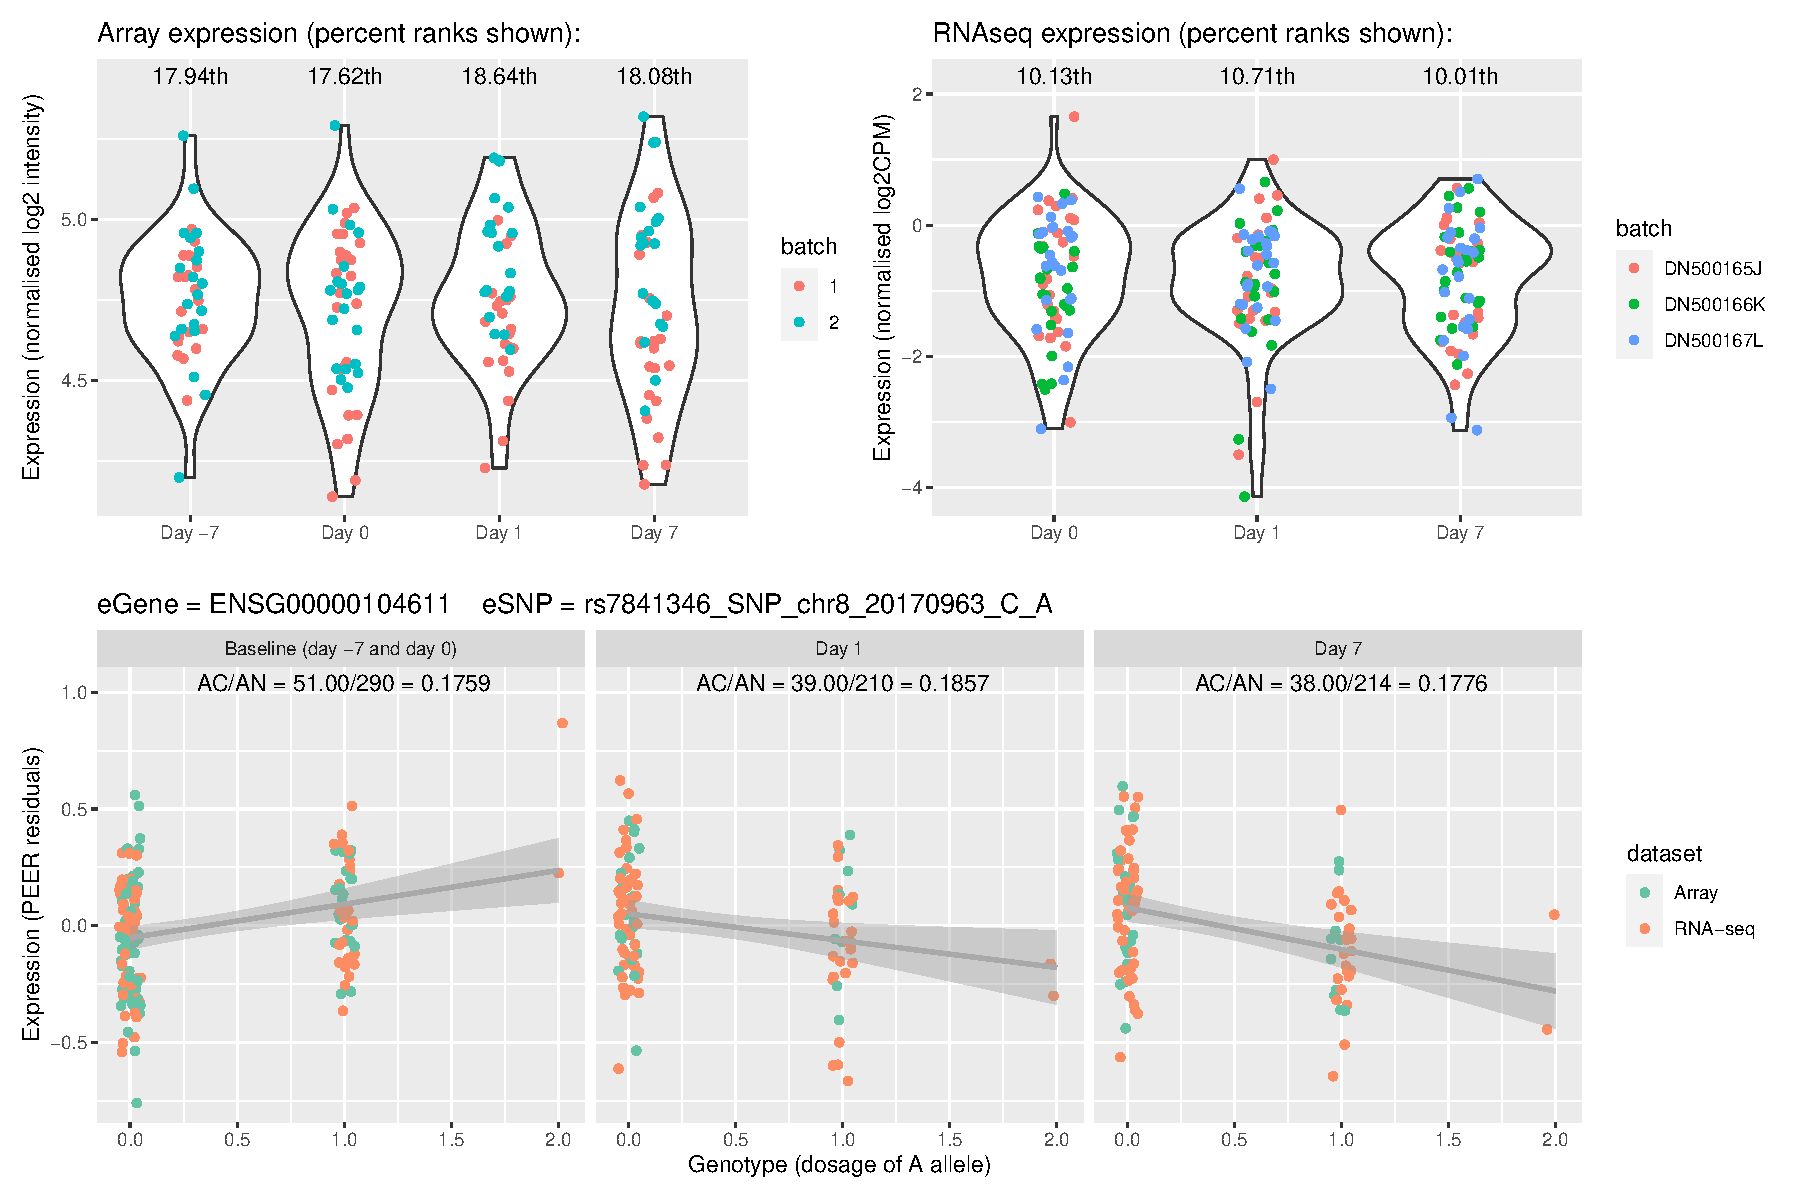
\includegraphics[width=1.0\textwidth,page=1]{mainmatter/figures/chapter_03/plot_dge_eqtl_genotypes.ENSG00000104611,rs7841346_SNP_chr8_20170963_C_A.pdf}
    \caption{
        \textbf{Expression and lead \gls{eQTL} of \gene{SH2D4A} over study timepoints.}
        Normalised array (top-left) and \gls{RNAseq} (top-right) expression before batch effect correction with ComBat.
        Bottom: \gls{eQTL} effects at each timepoint condition in the mega-analysis of array and \gls{RNAseq} data.
    }
    \label{fig:hird_eQTL_ploteQTL_SH2D4A}
\end{figure}

\subsubsection{Genotype by cell type interaction effects}

The presence of cell type-specific \gls{eQTL} effects was considered as an alternate explanation.
Even if an eGene is not differentially expressed on average in bulk expression data, 
the composition of cell types that are the source of that gene's transcripts can change.
\software{xCell} enrichment scores were used to approximate abundance of seven \gls{PBMC} cell types from the expression data.
After pruning highly correlated cell types to avoid multicollinearity, standardised scores for monocytes, \gls{NK} cells and plasma cells were tested for genotype interactions.
Within each timepoint, full \gls{eQTL} models including the genotype main effect, the three cell type abundance main effects, and three cell type-genotype interaction terms, were fit using \software{lme4qtl}, 
then compared to a nested model excluding the three interaction terms with an \gls{LRT}.
% The nested model has the same form as the within-timepoint models used in the main \gls{reQTL} analyses.
Significant cell type interactions were detected at \num{16/1154} \glspl{reQTL}-gene pairs in at least one timepoint (\gls{BH} \gls{FDR} < 0.05).
Fifteen were significant in only one timepoint:
baseline (\gene{SLAMF8}, \gene{CSE1L}, \gene{MAST1}, \gene{DLGAP1}),
day 1 (\gene{ZNF519}, \gene{LPAR1}, \gene{ADCY3}, \gene{NAA20}, \gene{EPB41L5}),
or day 7 (\gene{APOL6}, \gene{ADAR}, \gene{ADAM17}, \gene{UHRF2}, \gene{MST1}, \gene{CUL1}).
% \gene{SMDT1} at both d0 and d7

% $\chi^2(3) = \num{26.290769}$,
For \gene{ADCY3} at day 1 (full vs. nested \gls{FDR} = \num{9.539518e-05}),
although the genotype effect was \num{0.255954767} (SE = \num{0.03339378}) in the nested model,
% 0.35803609 \pm 0.05570632 limix
% 0.13549316 \pm 0.03266963 mashr
the estimate in the full model was \num{-0.007216815} (\num{0.06656115});
with the three cell type-genotype interaction term estimates being
\num{0.212978154} (\num{0.04897962}) for monocytes,
\num{-0.009195402} (\num{0.04470412}) for \gls{NK} cells,
and \num{0.016151511} (\num{0.06632921}) for plasma cells.
The small magnitude of the genotype main effect in the full model compared to the nested model suggests the \gls{eQTL} effect is driven largely by the monocyte score (or a cell type that is highly correlated with monocyte score in \cref{fig:hird_xCell_correlationMatrix}).
In the case where the monocyte score is zero (representing an average abundance across samples, as scores are standardised), the effect of increasing genotype dosage on \gene{ADCY3} expression is minimal.
\cref{fig:hird_reQTL_ADCY3_vs_monocyte_baseline,fig:hird_reQTL_ADCY3_vs_monocyte_day1} illustrate this effect.
Monocyte abundance has no effect on expression at baseline, 
increases after vaccination, and modifies the effect of genotype on expression at day 1.
It is feasible that the mechanism generating \gls{reQTL} at the remainder of these genes also involve cell type-specific \gls{eQTL} effects, 
but unlike at \gene{ADCY3}, 
I have not yet examined which of the three cell abundance scores have the greatest contribution.

\begin{figure}
    \centering
    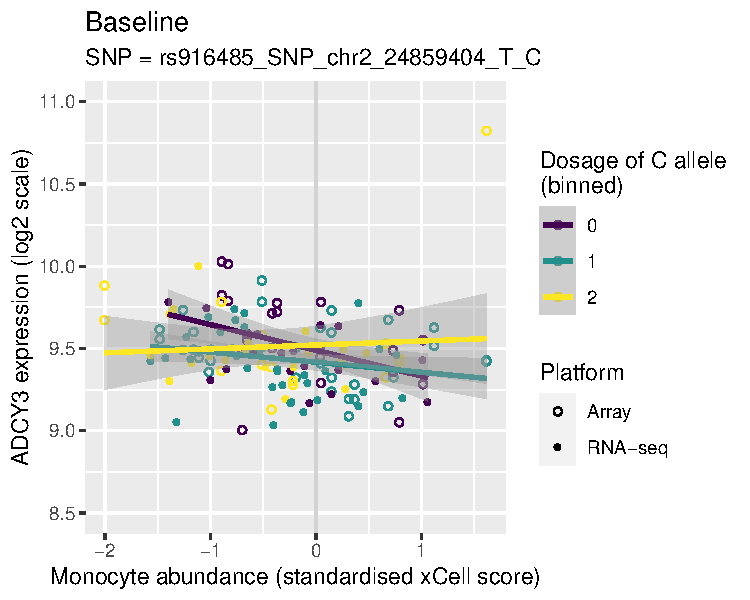
\includegraphics[width=1.0\textwidth,page=1]{mainmatter/figures/chapter_03/lme4qtl.ENSG00000138031_Monocyte_baseline.pdf}
    \caption{
        \textbf{Effect of estimated monocyte abundance on \gene{ADCY3} expression at baseline, stratified by genotype at a day 1 \gene{ADCY3} \gls{reQTL}.}
    }
    \label{fig:hird_reQTL_ADCY3_vs_monocyte_baseline}
\end{figure}

\begin{figure}
    \centering
    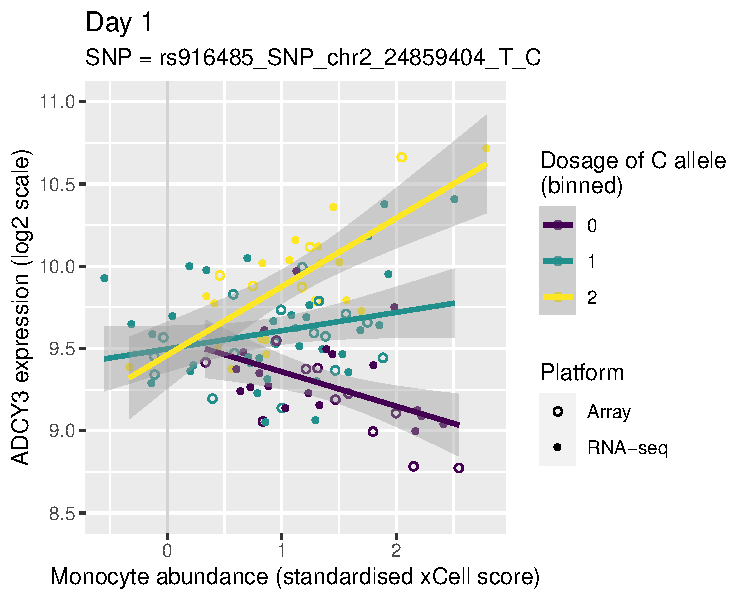
\includegraphics[width=1.0\textwidth,page=1]{mainmatter/figures/chapter_03/lme4qtl.ENSG00000138031_Monocyte_day1.pdf}
    \caption{
        \textbf{Effect of estimated monocyte abundance on \gene{ADCY3} expression at day 1, stratified by genotype at a day 1 \gene{ADCY3} \gls{reQTL}.}
    }
    \label{fig:hird_reQTL_ADCY3_vs_monocyte_day1}
\end{figure}

% \subsection{TODO Genotype by platform interaction effects}
%
% pull platform interaction in as a filter
%
% potential problems with mega discussed b4
% - platform fx
% - Using a fixed effect assumes mean diff between rnaseq and array and forces the slope to the average.
% - lme4qtl interactions with bonferroni
% - Perhaps using platform specific effects as a filter for reQTLs.
%
% \todo{Need to consider Nikos' comment that there are too many (1069/13570 significant BH FDR) genotype-platform interactions to use mega-analysis. Consider filtering.}

\subsubsection{Colocalisation with external QTL datasets at the \gene{ADCY3} locus}
\todo{new section}

The day 1 \gene{ADCY3} \gls{reQTL} is of particular interest,
as similar blood \gls{reQTL} after stimulation with \gls{TIV} \autocite{franco2013IntegrativeGenomicAnalysis}, rhinovirus \autocite{caliskan2015HostGeneticVariation}, and \textit{Mycobacterium leprae} \autocite{manry2017DecipheringGeneticControl}.
% NOTE: Also in obesity and T2D
The locus that contains the \gene{ADCY3} \gls{reQTL} has also been implicated in disease risk for \glspl{IMID} such as \gls{IBD} \autocite{delange2017GenomewideAssociationStudy},
and \gene{ADCY3} expression in immune cells in gut mucosa has been suggested to contribute to \gls{CD} risk (a subtype of \gls{IBD}) \autocite{marigorta2017TranscriptionalRiskScores}.
Aside from monocytes, \gene{ADCY3} is expressed in a wide range of immune cells---CD4\textsuperscript{+} T cells, CD8\textsuperscript{+} T cells, B cells, and \gls{NK} cells (\cref{fig:hird_eQTL_ADCY3_expression_DICE}).
Identifying cell type-dependent \gls{eQTL} through genotype-cell type abundance interaction terms cannot distinguish between cell types with highly correlated abundances \autocite{kim-hellmuth2020CellTypeSpecific}.
The high contributions to the same \gls{PC} for monocyte, CD4\textsuperscript{+} T cell, and CD8\textsuperscript{+} T cell xCell scores in the \gls{PCA} xCell scores indicates cell types with high \gene{ADCY3} expression are indeed correlated in \gls{HIRD} (\cref{fig:hird_xCell_cos2}).
Given the locus is associated with response to a wide range of immune stimuli, and also an \gls{IMID},
I conducted colocalisation analysis to test if shared causal variants 
may be driving these associations and to determine which of the correlated cell types expressing \gene{ADCY3} are mostly likely responsible.

\begin{figure}
    \centering
    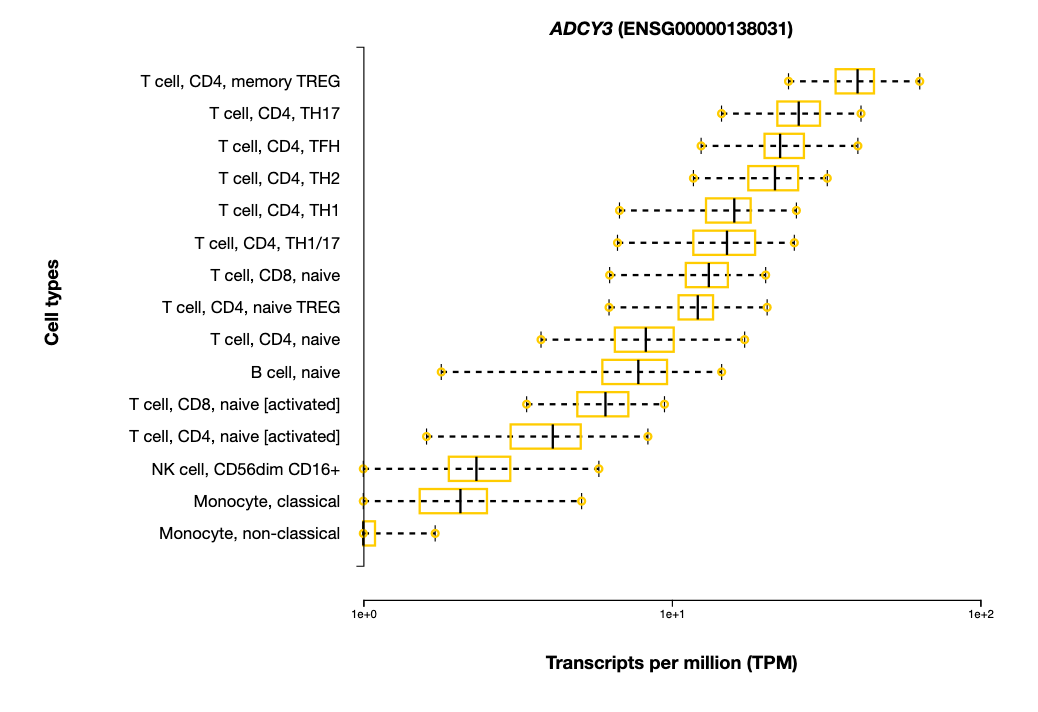
\includegraphics[width=1.0\textwidth,page=1]{mainmatter/figures/chapter_03/ADCY3_expression.png}
    \caption{
        \textbf{Expression of \gene{ADCY3} in sorted immune cell subsets.}
        \textcite{schmiedel2018ImpactGeneticPolymorphisms}, 
        \textit{DICE (database of immune cell expression, expression quantitative trait loci, and epigenomics}, 
        \url{https://dice-database.org/genes/ADCY3}, accessed Nov 2020.
    }
    \label{fig:hird_eQTL_ADCY3_expression_DICE}
\end{figure}

% rs916485_SNP_chr2_24859404_T_C
In a \SI{\pm 500}{\mega\bp} window around the lead \gls{reQTL} variant rs916485,
I performed Bayesian multi-trait colocalisation (\software{HyPrColoc} \autocite{foley2019FastEfficientColocalization}) of
the three per-timepoint \gene{ADCY3} \gls{eQTL} summary statistics with external datasets:
\gene{ADCY3} \gls{eQTL} from 15 sorted immune cell populations from \textcite{schmiedel2018ImpactGeneticPolymorphisms},
monocyte count \gls{QTL} from \textcite{astle2016AllelicLandscapeHuman},
and \gls{IBD} \gls{GWAS} from \textcite{delange2017GenomewideAssociationStudy}.
There were 1054 variants present in all 20 sets of summary statistics.

\software{HyPrColoc} identifies clusters of traits that colocalise at different causal variants in the locus.
As Bayesian colocalisation can be sensitive to the choice of priors,
I performed a sensitivity analysis iterating over configurations of priors and other algorithm parameters, ranging from default to more stringent parameter values.
Two stable clusters were identified across 100 configurations of parameters (\cref{fig:hird_reQTL_coloc_ADCY3_sensitivityPlotCustom}).
A set of three traits---\gene{ADCY3} expression in \gls{HIRD} day 1 and in naive classical and non-classical monocytes---clustered in \textapprox{\SI{65}{\percent}} of tested configurations.
A set of nine traits---\gls{IBD} and expression in eight naive and memory CD4+ T cell subsets---clustered in \textapprox{\SI{90}{\percent}} of tested configurations.
The remaining traits did not robustly cluster with any other traits over the tested configurations,
except for the rare inclusion of \gls{HIRD} baseline \gene{ADCY3} expression into the larger cluster for less stringent configurations.

% ADCY3 TSS is at 24919839, rev strand
%
% posterior_prob regional_prob candidate_snp posterior_explained_by_snp
%
% IBD T cell
% 0.9778        1.0000  2_24935139_C                          1
% rs713586 2:24935139 T C 
% 15300 upstream
%
% HIRD monocyte
% 0.9424        1.0000  2_24874083_C                          1
% rs7567997 2:24874083 T C
% 45756 downstream
%
The value of \software{prior.2} (the probability that a variant associated with at least one trait is not associated with any additional traits) was subsequently set to 0.99 (default = 0.98), 
sufficient to prevent clustering of baseline \gls{HIRD} expression with T cell and \gls{IBD}
The values of other priors and algorithm parameters were left at their defaults.
Under this configuration, the posterior probability that all traits in the cluster share a causal variant was \num{0.9778} for the larger cluster, 
and \num{0.9424} for the smaller cluster.
Distinct candidate causal variants were proposed for each cluster (\cref{fig:hird_reQTL_coloc_ADCY3_locusPlot}).
For the larger cluster, rs713586, a variant \SI{15}{\kilo\bp} upstream of the canonical \gene{ADCY3} \gls{TSS};
and for the smaller cluster, rs7567997, an intronic variant \SI{45}{\kilo\bp} downstream of the \gls{TSS}.
In both cases, the variant explained all of the posterior probability for the cluster, 
but as the analysis is restricted to the 1054 variants present in all datasets, there is ample chance the true causal variants were not included.

\begin{figure}
    \centering
    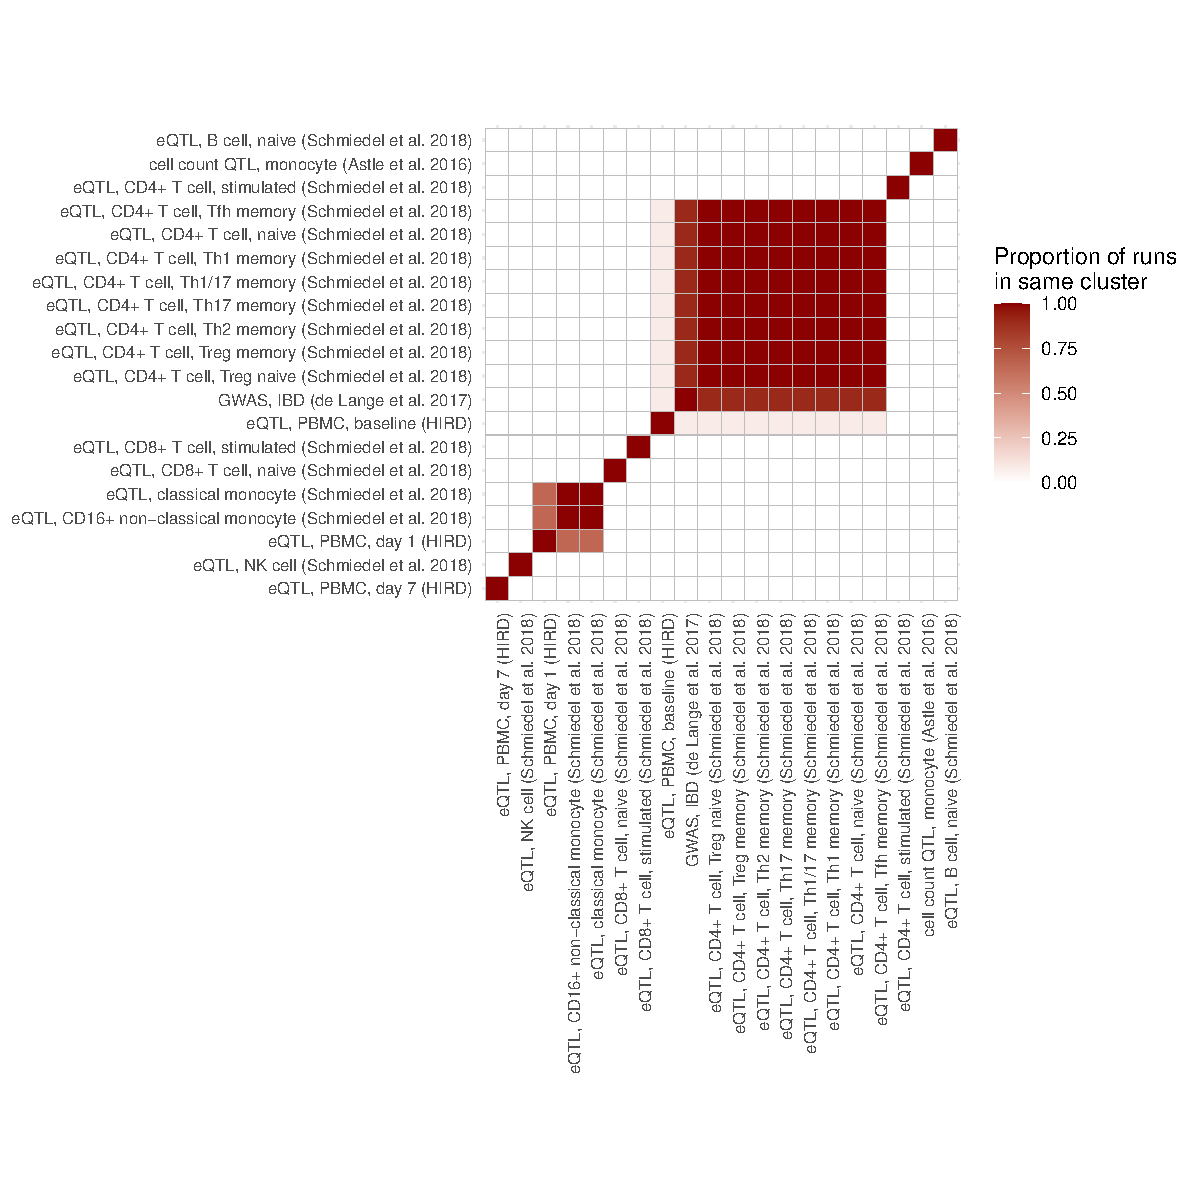
\includegraphics[width=1.0\textwidth,page=1]{mainmatter/figures/chapter_03/perform_coloc.gene_ENSG00000138031.sensitivityPlot_custom.pdf}
    \caption{
        \textbf{Sensitivity analysis for multi-trait colocalisation at the \gene{ADCY3} locus.}
        Colocalisation done using \software{HyPrColoc} \autocite{foley2019FastEfficientColocalization} in a 500 Kb window around the lead variant for the day 1 \gene{ADCY3} \gls{reQTL} in \gls{HIRD} for trait datasets described in \cref{subsec:hird_reQTL_coloc}.
        Heatmap shows the proportion of configurations in which two traits colocalise in the same cluster over 100 configurations of algorithm parameters
        \software{reg.thresh}, \software{align.thresh}, and \software{prior.2} (range of values listed in \cref{subsec:hird_reQTL_coloc}).
        \software{prior.1} set at \num{1e-4} (default).
        Rows and columns hierarchically-clustered.
    }
    \label{fig:hird_reQTL_coloc_ADCY3_sensitivityPlotCustom}
\end{figure}

\begin{figure}
    \centering
    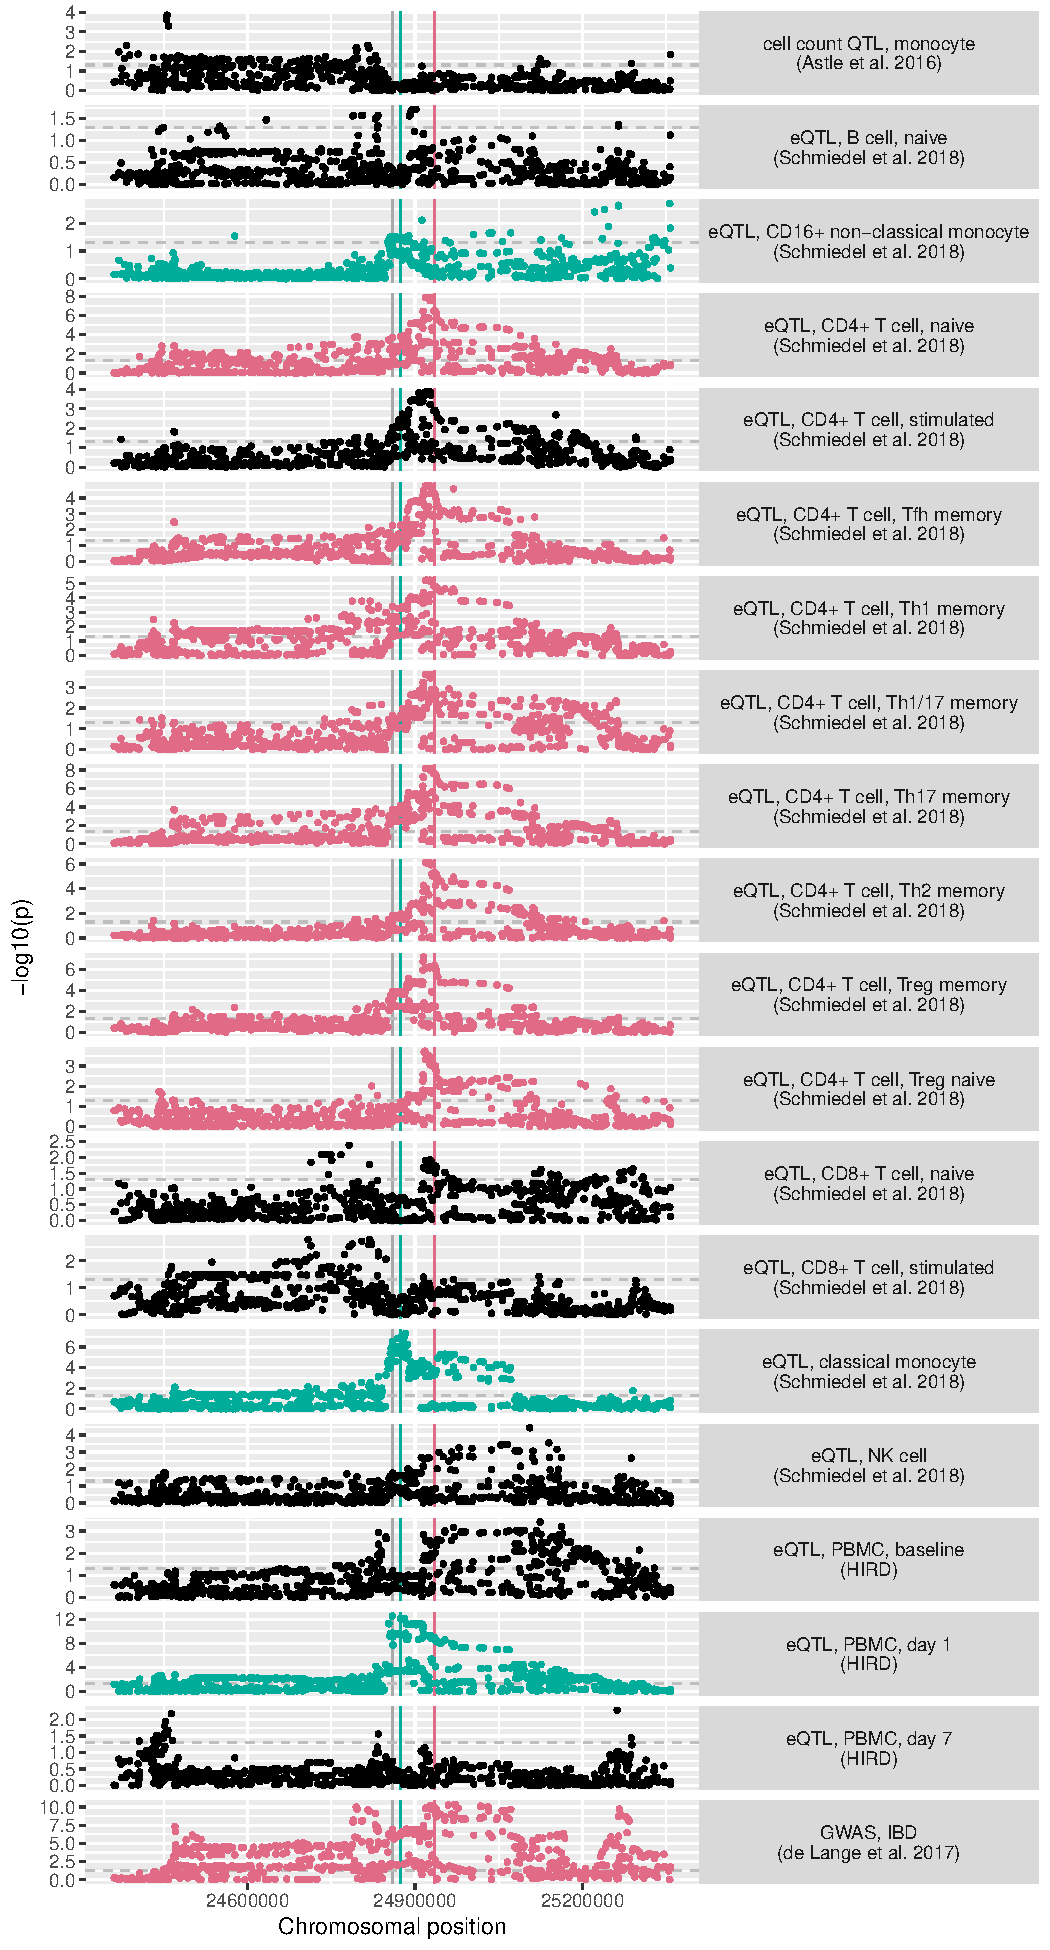
\includegraphics[width=1.0\textwidth,page=1]{mainmatter/figures/chapter_03/perform_coloc.gene_ENSG00000138031.locusPlot.pdf}
    \caption{
        \textbf{Multi-trait colocalisation at the \gene{ADCY3} locus.}
        Colocalisation done using \software{HyPrColoc} \autocite{foley2019FastEfficientColocalization} in a 500 Kb window around the lead variant for the day 1 \gene{ADCY3} \gls{reQTL} in \gls{HIRD} (vertical grey line).
        Traits are monocyte cell count (\textcite{astle2016AllelicLandscapeHuman}), \gene{ADCY3} expression in sorted immune cell subsets (\textcite{schmiedel2018ImpactGeneticPolymorphisms}), \gene{ADCY3} expression in \gls{HIRD} timepoints, and \gls{IBD} (\textcite{delange2017GenomewideAssociationStudy}).
        Locus plots show summary statistics for 1054 variants present in all datasets.
        Traits in red and green represent two distinct clusters each hypothesised to be driven by a shared causal variant (vertical red and green lines).
        Non-colocalising traits are shown in black.
        Horizontal dashed line shows p = 0.05.
        Default values for priors and algorithm parameters used, except \software{prior.2} = 0.99.
    }
    \label{fig:hird_reQTL_coloc_ADCY3_locusPlot}
\end{figure}

Nevertheless, the two main clusters being distinct from one another, and from non-colocalising traits across many configurations,
still supports the existence of distinct causal variants, even if they may be unobserved.
For \gls{HIRD} day 1 expression of \gene{ADCY3}, the more relevant cell type appears to be monocytes, not a correlated cell type like CD4\textsuperscript{+} T cells---and vice versa for \gls{IBD}.
The clustering was robust despite the data containing no stimulated monocyte subsets.
This \gls{eQTL} effect is readily observable at baseline, and appears to be more significant in naive classical than non-classical monocytes in the \autocite{schmiedel2018ImpactGeneticPolymorphisms} data (\cref{fig:hird_reQTL_coloc_ADCY3_locusPlot}).
No colocalisation with blood monocyte count was observed, 
so the \gls{reQTL} does not appear to affect monocyte abundance in general.
I believe a variant that affects ability to increase monocyte counts post-vaccination can also be ruled out,
as in that case the effect of genotype on expression is entirely mediated through the effect of genotype on monocyte abundance,
so having cell abundances as covariates in the regression should eliminate that effect.
Thus I hypothesise that a plausible mechanism generating the day 1 \gls{reQTL} signal in \gls{HIRD}
is an increase in abundance of classical monocytes at day 1 post-vaccination,
increasing the proportion of \gene{ADCY3} transcripts in the bulk data originating from monocytes,
thus making an \gls{eQTL} specific to monocytes--not just stimulated monocytes---more readily detectable.
This is the scenario where monocyte abundance modifies the effect of genotype on expression.

\section{Discussion}

Just as vaccination was found to induce extensive changes in the transcriptome
in \cref{ch:hird_DGE},
it also induces changes in the regulatory architecture of gene expression.
In a mega-analysis of array and \gls{RNAseq} datasets,
\textit{cis}-\gls{eQTL} were detected for \percentage{0.5075166} (\num{6887/13570}) of genes in at least one timepoint,
and the majority replicated in the much larger GTEx whole blood dataset.
This is a substantial eGene rate given the modest per-timepoint sample size in \gls{HIRD}, reflecting the gain in effective sample size from joint mapping over multiple conditions.
% Each method for determining reQTL has its own biases.
% Even in a joint mapping framework, defining \gls{reQTL} by set significance thresholds, or change in the amount of expression variation explained, will miss classifying equal but opposite effect sizes.
Defining reQTL from a significant difference in beta of the same \gls{eQTL} between timepoints,
\num{1154/6887} (\percentage{0.1675621}) of lead \gls{eQTL} were classified as \gls{reQTL}.
This is comparable to estimates of \SIrange{3}{18}{\%} \gls{reQTL} between monocytes in different stimulation conditions by \textcite{kim-hellmuth2017GeneticRegulatoryEffects} who also used a beta comparison approach.
The method is relatively stringent at calling \gls{reQTL},
avoiding both threshold effects where significant and non-significant \gls{eQTL} may have very similar betas,
and discovery power biases caused by sample size differences between conditions.
Indeed, had \gls{reQTL} been called by significance alone, 1427 \gls{reQTL} would have been detected just at baseline, the timepoint with the largest sample size in \gls{HIRD}.
There is a growing consensus in the literature that most \gls{eQTL} are shared between conditions such as tissue and cell-type \autocite{ongen2017EstimatingCausalTissues,urbut2018FlexibleStatisticalMethods,kim-hellmuth2020CellTypeSpecific,umans2020WhereAreDiseaseAssociated},
% TODO: check fairfax2012GeneticsGeneExpression
% We identified 82,346 eQTL (SNP-probe interactions, referred to hereafter as eSNPs) at permuted p<0.001, 32.2% of which were unique to B-cells, 45.9% to monocytes and 21.8% shared between cell types
and that high estimates of 50\% or more condition-specificity based on significance thresholds (e.g. \autocite{ackermann2013ImpactNaturalGenetic}) are overestimated.
A counter-argument is that many studies overestimate sharing by calling condition-specific effects in \gls{LD} as shared \autocite{umans2020WhereAreDiseaseAssociated}.
Here I compared the same gene-tag \gls{SNP} pair across timepoints,
but distinct causal and condition-specific variants may be tagged in such a way that the effect size of the tag \gls{SNP} ends up similar---multi-trait colocalisation would be required to truly confirm a shared \gls{eQTL}.

Gene set enrichment analyses to identify shared biological processes among target genes for \gls{reQTL} were generally uninformative.
Genes targeted by \gls{reQTL} that explained more variation in expression post-vaccination were enriched for immune activation, with weaker enrichments related to \gls{APC}.
This misses the full picture though, as many of the strongest \gls{reQTL} were those with opposite sign effects at baseline and post-vaccination not captured by changes in \gls{PVE}.
Prevalence of opposite sign effects between pairs of conditions has been previously described in multi-tissue studies;
in \textcite{fu2012UnravelingRegulatoryMechanisms}, the proportion of opposite sign effects among all reQTLs between five tissues was \percentage{0.044}.
In \gls{HIRD}, I found an unexpectedly high proportion:
39/819 (\percentage{0.04761905}) for day 1 \gls{reQTL},
and 211/1002 (\percentage{0.2105788}) for day 7 \gls{reQTL}.
% TODO: get fairfax2012GeneticsGeneExpression figure
% TODO: recheck no cell type enrichments in these two sets of reQTL
% but it is unclear how this may lead to generation of opposite effects, and
% \todo{ check "rs2223286 is associated with profound directional effects in
% the expression of SELL dependent upon genotype, with the minor C allele
% associated with increased expression of SELL in B-cells and reduced
% expression of SELL in monocytes " }
Given the larger global changes in expression vs. baseline at day 1 compared to
day 7 described in \cref{ch:hird_DGE}, 
the larger number of strong \glspl{reQTL} at day 7 was also unexpected.
% In \autocite{mizuno2019BiologicalCharacterizationExpression}, the proportion of opposite sign effects as a percentage of all eGenes was \percentage{0.074} (48 tissues);
% in \gls{HIRD}, I find
% 39/6887 (\percentage{0.005662843}) at day 1,
% and 211/6887 (\percentage{0.03063743}) at day 7.

Post-vaccination \gls{DGE} was considered as a mechanism that might generate \gls{reQTL}.
As in \textcite{kim-hellmuth2017GeneticRegulatoryEffects, davenport2018DiscoveringVivoCytokineeQTL}, the overlap between \gls{DGE} and genes with reQTL in \gls{HIRD} was poor.
Only at day 7 were \gls{reQTL} more likely to be differentially expressed than genes without reQTL, specifically when restricting the analysis to eGenes.
Those day 7 \gls{reQTL} that were also upregulated at day 7 were enriched in cell cycle Gene Ontology sets, but it is unclear how this may lead to generation of opposite effects, and the enrichment may largely be driven by the \gls{DGE} signal rather than the \gls{reQTL} one.
To define genes important to \gls{TIV} response,
\textcite{franco2013IntegrativeGenomicAnalysis} made heavy use of the overlap of \gls{DGE} and \gls{eQTL}, followed by gene set enrichment.
Unfortunately, their overlap criteria before enrichment covered genes with either \gls{DGE} \emph{or} \gls{reQTL}, so it is difficult to assess 
which contributed more to their significant enrichments in the antigen presentation pathway.
% 20 genes from Franco
% 12/17 DGE replicated
% 14/17 eGenes replicated, none were reQTL
% \todo{dge is coupled to reqtl, if you do an enrichment of dge+reqtl overlap genes, likely their enrichment is driven by DGE signal}
As noted by \textcite{davenport2018DiscoveringVivoCytokineeQTL,cuomo2020SinglecellRNAsequencingDifferentiating}, 
it may be that \gls{DGE} and \gls{reQTL} are generated by different mechanisms, and focusing on the overlap is an unnecessarily narrow view. 

An unappealing thought is that opposite sign effects are enriched in false positives, especially as they seem to show no positional enrichment near the \gls{TSS}.
While it is known that stimulation-specific \gls{reQTL} are more distal than baseline eQTL \autocite{fairfax2014InnateImmuneActivity}, the \gls{HIRD} reQTL are evenly spread across the cis- window.
Some reQTL may be statistical artifacts of the shrinkage of effects by \software{mashr}.
Small and opposite effects generated by noise may be frequent enough for \software{mashr} to consider them a \enquote{pattern} of effects.
This might explain the clear separation of the distribution of z-statistics for difference in beta between \gls{reQTL} and shared eQTLs.
Conversely, it may be that small and opposite effects are more prevalent than expected, and this is the best framework for detecting them.
% This may be a consequence of the beta comparison approach, as opposite sign of effect tends to result in greater difference in betas.
% TODO: need to consider changes in effect and sign, not just significance
To confirm either way, it may be necessary to repeat the \gls{reQTL} calling without the benefit of \software{mashr} shrinkage in a different modelling framework,
such as a timepoint-genotype interaction term \autocite{davenport2018DiscoveringVivoCytokineeQTL}.
A complementary approach for validating these opposite sign \gls{reQTL} using the existing \gls{RNAseq} data might be within-individual \gls{ASE} (e.g. RASQUAL \autocite{kumasaka2016FinemappingCellularQTLs}),
which can be performed with the same data types as \gls{eQTL} mapping,
% \todo{switch to Allele-Specific QTL Fine Mapping with PLASMA}
and where one would expect true opposite sign \gls{reQTL} effects would also be recapitulated as opposite directions of allelic expression imbalance.
\gls{ASE} may also provide more interpretable effect sizes than \gls{eQTL} betas \autocite{mohammadi2017QuantifyingRegulatoryEffect},
for purposes such as clustering effect sizes to determine patterns of effects across timepoints \autocite{cuomo2020SinglecellRNAsequencingDifferentiating}.

At least one \gls{reQTL} signal was plausibly not a false positive.
\todo{phew.}
The strongest \gls{reQTL} detected at day 1 was for \gene{ADCY3}, a membrane-bound enzyme that catalyses the conversion of ATP to the second messenger cAMP \autocite{wu2016AdenylateCyclaseNew}.
% During the process of ‘tolerance/immunoparalysis’, a common complication of severe sepsis, monocytes enter a refractory functional state, characterized by the incapacity to produce proinflammatory cytokines and decreased HLA-DR expression (9). Tolerance can be mimicked in vitro and in vivo by challenging the cells with endotoxins such as LPS: after an initial stimulation phase, cells enter a state of long-term immunotolerance. In contrast, other infections or vaccinations (e.g. Candida albicans infection, Bacille Calmette-Guerin (BCG) or measles vaccination) increase the long-term responsiveness of monocytes to microbial stimuli, a state termed ‘trained immunity’ which confers resistance to secondary infections (10–14).
\gene{ADCY3} is upregulated after the differentiation of monocytes induced by beta-glucan,
into macrophages in a state of trained immunity---a state in which they are more responsive to future immune stimuli \autocite{saeed2014EpigeneticProgrammingMonocytetomacrophage}.
\Glspl{GWAS} have implicated the \gene{ADCY3} locus for diseases such as obesity \autocite{wu2016AdenylateCyclaseNew} and \gls{IBD} \autocite{delange2017GenomewideAssociationStudy}.
\gene{ADCY3} has also been identified as a post-stimulation \gls{reQTL} in other studies involving stimulated blood immune cells:
% In fact, six (SLFN5, ARL5B, SPTLC2, IRF5, ADCY3, CCDC146) of the 38 genes
% implicated in our reQTL mapping were also identified in a recent reQTL mapping
% study for Escherichia coli lipopolysaccharide, influenza, and interferon-β in
% dendritic cells [35].
in \gls{PBMC} 24h after \textit{in vitro} infection with rhinovirus \autocite{caliskan2015HostGeneticVariation},
in whole blood \textit{in vivo} day 1 after vaccination with seasonal \gls{TIV} \autocite{franco2013IntegrativeGenomicAnalysis},
% Examples of three reQTL among genes found only in M. leprae sonicate stimulated
% cells or non-stimulated cells. For each gene ((A) ADCY3, (B) DNAAF1 and (C)
% ZNF517): the left panel corresponds to the expression of the gene in
% non-stimulated cells while the right panel depicts expression of the gene in
% stimulated cells. The gene identity is indicated above each pair of graphs. The
% gene expression level in log2 scale (y-axis) is plotted for each genotype
% (x-axis). Of note, reQTL for the ADCY3 and DNAAF1 genes have been found by
% other studies using distinct pathogens or molecules as stimuli, while the reQTL
% for ZNF517 is a newly identified reQTL [21, 22, 24, 26]. ADCY3 is among the
% most upregulated genes after stimulation with M. leprae antigens and has been
% identified as part of the T1R gene set signature identified by Orlova et al.
% [32]. The reQTL for DNAAF1 displays the strongest p value among the reQTL we
% identified.
and in whole blood after \textit{in vitro} stimulation with \text{M. leprae antigen} for 26-32 h \autocite{manry2017DecipheringGeneticControl}.
% TODO:
% Aside from \gene{ADCY3}, I also see \autocite{caliskan2015HostGeneticVariation} a day 1 reQTL at \gene{SLFN5} (PVE increase from \num{0.27048709} to \num{3.386358e-01}, p diff = \num{4.882379e-02}). , but no upreg
%
Given the diversity of stimulations and tissue types, the effect is likely a consequence of general immune activation, rather than a Pandemrix-specific response.

% TODO: do we fall into the Table 2 Fallacy? we should not interpret cell count estiamte params as causal effects, but moderation is demonstrable
% http://www.dagitty.net/learn/graphs/table2-fallacy.html
%
The strength of the \gene{ADCY3} \gls{reQTL} at day 1 was found to be modified by xCell estimates of monocyte abundance. 
% Changes in relative abundances for many cell types occur in the bulk PBMC samples after vaccination.
% I accounted for the effect of abundance on mean expression including xCell scores and PEER factors as fixed effects in the model,
% and also considered the effect of abundance on the genotype effect using interaction terms between xCell scores and genotype.
% Due to the modest sample size, and computational requirements for \software{lme4qtl},
% I focused only whether reQTLs that have a detectable main effect may be driven by cell type interactions,
% testing only for interactions at significant lead \gls{reQTL},
%
The xCell scores are imperfect.
Compared to FACS measurements in a cohort subset, the xCell scores were only weakly correlated, and the signatures used by xCell may be less accurate after vaccine stimulation.
Fortunately, statistical colocalisation confirms that the day 1 reQTL signal identified for \gene{ADCY3} is likely to be a monocyte-specific effect---and independent to the IBD signal in the locus, which colocalises with CD4 T cell eQTL datasets.
The proportion of monocytes in the \gls{PBMC} compartment increases at day 1, supported by both FACS \autocite{sobolev2016AdjuvantedInfluenzaH1N1Vaccination} measurements, and an increase in monocyte xCell score.
Expression of \gene{ADCY3} is not monocyte-specific: despite the increase in monocyte proportion, no upregulation was observed at day 1.
Colocalisation was also not restricted to stimulated monocytes.
The probable mechanism is an increased proportion of the bulk sample taken up by monocytes at day 1 providing more monocyte-derived \gene{ADCY3} transcripts,
rather than a upregulation-driven increase in detection power,
or a vaccine-induced activation of the locus at day 1.
Although multi-trait colocalisation proved to be the crucial piece of evidence suggesting the effect is not related to T cells,
only 15 immune cell types were included in the analysis, so it is possible the reQTL is not entirely monocyte specific.

%
% TODO:
% how to get multi ethnic coloc?
% o	check ancestries of coloced populations: how does trans-ethnic fine mapping work?
%  how to get coloc priors, fgwas (cano 2020), enloc (kim-hell 2020)?
%
%Tastle european
%Third multi, 70% eu
%Tdice is multi ethnic san diego, 50% white eu, 
%Tfairfax european 
% gtex largely eu before v8
% Coloc
% \2 Biases from ethnicity-derived differences in LD?
    % T cell vs monocyte distinghish since both same from DICE
% Assumptions
% multiethnic
% 1 causal per (cluster/trait), untrue in any bulk
% \todo{re: the issue of discussing only top hits: hard to resolve due to the lack of gene set enrichments and time, but hopefully discussion about sets of genes with shared generating mechanisms might work}

% TODO: need to consider more cell types one by one?

% TODO:
% Still do not know causal variant
% or mechanism here
% no fine mapping

Overall, cell type interactions were only detected at 16/1154 reQTLs.
% the genotype effect was detected to interact with abundance of one or more of the tested cell types (or a correlated cell type).
Although power to detect significant interactions is lower than power to detect main effects,
not helped by the unclear reliability of xCell scores,
it is still likely that mechanisms other than shifts in cell abundance underlie a large number of the detected reQTLs.
% A pressing question remains: what molecular mechanisms underlie the \gene{ADCY3} \gls{reQTL}, and indeed the remainder of the \glspl{reQTL}?
One type of mechanism by which cis-eQTL affect expression is through their impact on \gls{TF} binding affinity to motifs in promoters and enhancers \autocite{pai2015GeneticMechanisticBasis}.
Immune cells, including monocytes, are heavily regulated by cell type-specific \glspl{TF} \autocite{choudhury2016IdentifyingCellTypeSpecific}.
Cell type-specific expression of different \glspl{TF} have been proposed as a model for explaining magnifying, dampening and opposite reQTL effects;
for example, opposite effects can result from \glspl{TF} regulating the same gene, that are activating in one cell type and suppressive in another \autocite{fu2012UnravelingRegulatoryMechanisms}.
There is evidence that \gls{TF} activity is important for \textit{in vivo} immune reQTL:
\autocite{caliskan2015HostGeneticVariation} found rhinovirus reQTLs in \glspl{PBMC} were enriched in ENCODE ChIP-seq peaks for the \glspl{TF} \gene{STAT1} and \gene{STAT2},
and \autocite{davenport2018DiscoveringVivoCytokineeQTL} found interferon and anti-IL6 drug reQTLs likely disrupt \gene{ISRE} and \gene{IRF4} binding motifs.
Rather than condition-specific expression of the eGene, what may be condition-specific is the expression of \glspl{TF} whose activity is affected by the reQTL.
A genomic feature enrichment for TF binding sites and other regulatory elements like enhancer regions among HIRD reQTL variants could expose shared regulatory factors that explain subsets of the remaining reQTL.
This would also help evaluate if the even distribution of reQTL across the \textit{cis}- window is a cause for concern.

%
% \footnote{
%     A cursory scan of \gls{TF} motifs disrupted by the location of the fine-mapped \gene{ADCY3} reQTL intronic variant rs13407913 on \url{https://ccg.epfl.ch/snp2tfbs/snpviewer.php},
%     does indeed show several motifs (for NR2C2, HNF4A, HNF4G, NR2F1)
%     where the PWM score is higher for the ALT allele,
%     consistent with the direction of effect for the day 1 reQTL.
% }.
% introns can be TF bound https://journals.plos.org/plosone/article?id=10.1371/journal.pone.0046784
% http://54.245.180.226/php_file/multiple.php?ID=rs13407913
% SP1 is monocyte specific https://europepmc.org/article/med/28008225
% and upreg at d1

Not only are the mechanisms at many detected reQTL unknown, there may be many more reQTL yet to detect.
% AND
% also i miss alot too...
%
% Also see for conditional:
% https://academic.oup.com/hmg/article/26/8/1444/2970473
% https://journals.plos.org/plosgenetics/article?id=10.1371/journal.pgen.1003649
Multiple independent eQTLs are present for a large fraction of eGenes \autocite{zeng2019ComprehensiveMultipleEQTL}.
% To sidestep the issue of multiple tested variants per gene being in \gls{LD},
% only lead , and same variatn
% NOte could be possible that the var still tags diff causal variants, would need fine mapping in each condition to confirm
% - misses secondary eQTL
% - misses multiple causal variants
As the lead variant for reQTL assessment for each eGene was chosen based on significance across all conditions, I can not detect reQTL that are masked by a stronger shared eQTL at that gene.
This is not expected to be uncommon, as the effective sample size for shared eQTLs is usually large due to borrowing of information across conditions.
% TODO
% https://www.biorxiv.org/content/10.1101/129429v2.full.pdf
% Primary 330eQTL fall closer to the TSS than conditional eQTL (Figure 2): primary eQTL 331occur at a median distance of 70.4 Kb from the TSS versus a median distance of 332302 Kb for conditional eQTL.
% TODO:
% It has been noted that distant \glspl{eQTL} have more context-specific effects \autocite{vandiedonck2017GeneticAssociationMolecular}.
Secondary \gls{eQTL} signals tend to be weaker, more distal to the TSS, more likely to be enriched in enhancers rather than promoters, and importantly, more context-specific\autocite{vandiedonck2017GeneticAssociationMolecular,dobbyn2018LandscapeConditionalEQTL,rotival2019CharacterisingGeneticBasis}.
% TODO:
% more distal: https://twitter.com/tuuliel_lab/status/1318979038346620928
The proportion of genes with reQTL I detect based on only the lead signal likely represents a lower bound.
Step-wise conditional analyses at each lead variant will be required to uncover secondary associations, 
which then can be compared across timepoints in the same manner as the primary associations.
These associations, although weaker on average, may actually have more variable effects between timepoints.
I also do not consider \textit{trans}-\gls{eQTL} due to sample size, which may be more likey to be condition specific than \textit{cis}-\gls{eQTL} \autocite{fairfax2012GeneticsGeneExpression,westra2014GenomeFunctionStudying,fairfax2014InnateImmuneActivity}.

% TODO: this is a only first step towards causality of delta expression
Finally, I address the prospect that common genetic variation may explain some variation in antibody response to Pandemrix.
% TODO
% Based on studies in twins, genetics seems to contribute only marginally to this heterogeneity
% in vaccination outcomes in adults, suggesting environmental factors as key drivers [19,20].
% tsang2020
I have indirectly demonstrated genotype-dependent effects on expression response by identifying reQTLs with differing effect size between timepoints,
% TODO
% Main point is causality is hard to define
% Even if Detect cell type specific eQTLs, not easy to say if the reQTL is important to vaccine response
but have yet to determine resulting genotype-dependent differences in antibody phenotypes.
Some of the identified reQTLs will undoubtedly affect genes whose expression or post-vaccination expression change correlates with antibody response, 
but correlation is not transitive \autocite{langford2001PropertyBeingPositively},
so correlation of genotype with expression and expression with antibody response does not imply a correlation between genotype and antibody response.
% \todo{note coloc doesn't distinguish pleiotropy from mediation?}
% many many scenarios possible: https://genomemedicine.biomedcentral.com/articles/10.1186/s13073-019-0613-2/figures/1
Formal tests such as the CIT \autocite{millstein2009DisentanglingMolecularRelationships} are required to distinguish mediation of genotype-antibody associations through gene expression from competing models.
\textcite{franco2013IntegrativeGenomicAnalysis} realised this, but concluded that they had insufficient power with a greater sample size and comparable study design to \gls{HIRD}.
The \gls{HIRD} cohort is also too small for a direct \gls{GWAS} of Pandemrix antibody response.
% TODO: after all that Intro about gwas to function, we unfortunately lack the gwas part here
A suitable approach for prioritising reQTL that contribute to the antibody response to Pandemrix will be to leverage external genetic associations to similar phenotypes,
for example, colocalisation with existing GWAS summary statistics for antibody response to a similar type of adjuvanted, inactivated vaccine.
%
% Even if ADCY3 is real is it interesting?
% is it important to vaccine response?
% TODO:
% \todo{need to consider: if this kind of thing is what bulk in vivo reQTL can find, they what is the additional value over FACS?}
% pressing 2: why even in vivo reqtl?
% TODO
% Basically, a utility of this is identification of cell type specific eQTLs from bulk
% We need a stimulation. ADCY3 is not detected as cell type eQTL at bulk even with monocyte term
% TODO:
% is ASE affected by cell comp?
% why specifically would ASE help?
%
Due to the number of possible generating mechanisms for bulk reQTL \textit{in vivo},
careful interpretation is required to gain any insight into the biology of the stimulation in question.
\cref{ch:discussion} will continue the discussion on the methodologies, experimental designs and upcoming technologies 
required to complement the \textit{in vivo} \gls{reQTL} design.
% TODO: add contribution to the field
\todo{i hope i can think of something convincing :p}

% TODO: another possiblility
% GARFIELD enrichment analysis21 showed that the cis-eSNPs were enriched in 3′ untranslated regions (UTR), 5′ UTR, and exon regions (Supplementary Fig. 4), consistent with known mechanisms of cis-eQTLs.

% \todo{add 1 concluding line}
% \todo{Overall I feel like the chapter is too descriptive, and falls short of
% making biological insights into Pandemrix response. Any additional analyses
% would hope to address that.}

% TODO: add a whilst we were not able to X in the intro, the field has advanced by Y, future Z needed

% TODO not scalable
% Would like to know what cell types for all reqtl, but limited by a trying one by one strategy
% Always might miss one not tried
% Not viable for scaling
% diff strat might be better like SC rnaseq

% PVE
%
% The \glspl{eQTL} with the highest \gls{PVE}\footnote{TODO: add to methods \url{https://journals.plos.org/plosone/article/file?type=supplementary&id=info:doi/10.1371/journal.pone.0120758.s001}}
% \todo{put pve formula in methods, include point that pve is (very rough) norm to var(y), so can compare between timepoints and genes with different MAF and raw variance}
% \todo{actually, i've found that my PVE approximation is basically rescaled abs(Z), so pve is a bit pointless if we already have z, and doesn't really help with comparability between genes with diff var/MAF}

% TODO: what does ADCY3 actually do in monocytes?
% https://www.ncbi.nlm.nih.gov/pmc/articles/PMC4242194/
